\documentclass[a4paper]{book}
\usepackage{makeidx}
\usepackage{natbib}
\usepackage{graphicx}
\usepackage{multicol}
\usepackage{float}
\usepackage{listings}
\usepackage{color}
\usepackage{ifthen}
\usepackage[table]{xcolor}
\usepackage{textcomp}
\usepackage{alltt}
\usepackage{ifpdf}
\ifpdf
\usepackage[pdftex,
            pagebackref=true,
            colorlinks=true,
            linkcolor=blue,
            unicode
           ]{hyperref}
\else
\usepackage[ps2pdf,
            pagebackref=true,
            colorlinks=true,
            linkcolor=blue,
            unicode
           ]{hyperref}
\usepackage{pspicture}
\fi
\usepackage[utf8]{inputenc}
\usepackage{mathptmx}
\usepackage[scaled=.90]{helvet}
\usepackage{courier}
\usepackage{sectsty}
\usepackage[titles]{tocloft}
\usepackage{doxygen}
\lstset{language=C++,inputencoding=utf8,basicstyle=\footnotesize,breaklines=true,breakatwhitespace=true,tabsize=4,numbers=left }
\makeindex
\setcounter{tocdepth}{3}
\renewcommand{\footrulewidth}{0.4pt}
\renewcommand{\familydefault}{\sfdefault}
\hfuzz=15pt
\setlength{\emergencystretch}{15pt}
\hbadness=750
\tolerance=750
\begin{document}
\hypersetup{pageanchor=false,citecolor=blue}
\begin{titlepage}
\vspace*{7cm}
\begin{center}
{\Large \-Task-\/\-Organizer }\\
\vspace*{1cm}
{\large \-Generated by Doxygen 1.7.5.1}\\
\vspace*{0.5cm}
{\small Wed Sep 28 2011 13:57:34}\\
\end{center}
\end{titlepage}
\clearemptydoublepage
\pagenumbering{roman}
\tableofcontents
\clearemptydoublepage
\pagenumbering{arabic}
\hypersetup{pageanchor=true,citecolor=blue}
\chapter{\-Namespace \-Index}
\section{\-Packages}
\-Here are the packages with brief descriptions (if available)\-:\begin{DoxyCompactList}
\item\contentsline{section}{\hyperlink{namespacecliparser}{cliparser} }{\pageref{namespacecliparser}}{}
\item\contentsline{section}{\hyperlink{namespacecontroller}{controller} }{\pageref{namespacecontroller}}{}
\item\contentsline{section}{\hyperlink{namespacectask}{ctask} }{\pageref{namespacectask}}{}
\item\contentsline{section}{\hyperlink{namespacelogger}{logger} }{\pageref{namespacelogger}}{}
\item\contentsline{section}{\hyperlink{namespacestorage}{storage} }{\pageref{namespacestorage}}{}
\item\contentsline{section}{\hyperlink{namespacetask}{task} }{\pageref{namespacetask}}{}
\item\contentsline{section}{\hyperlink{namespacetest__cliparser}{test\-\_\-cliparser} }{\pageref{namespacetest__cliparser}}{}
\item\contentsline{section}{\hyperlink{namespacetest__task}{test\-\_\-task} }{\pageref{namespacetest__task}}{}
\item\contentsline{section}{\hyperlink{namespacetest__taskcontroller}{test\-\_\-taskcontroller} }{\pageref{namespacetest__taskcontroller}}{}
\item\contentsline{section}{\hyperlink{namespacetest__taskstorage}{test\-\_\-taskstorage} }{\pageref{namespacetest__taskstorage}}{}
\item\contentsline{section}{\hyperlink{namespaceutil}{util} }{\pageref{namespaceutil}}{}
\end{DoxyCompactList}

\chapter{\-Class \-Index}
\section{\-Class \-Hierarchy}
\-This inheritance list is sorted roughly, but not completely, alphabetically\-:\begin{DoxyCompactList}
\item \contentsline{section}{storage\-:\-:\-\_\-\-Key\-Generator}{\pageref{classstorage_1_1__KeyGenerator}}{}
\item \contentsline{section}{cliparser\-:\-:\-C\-L\-I\-Parser}{\pageref{classcliparser_1_1CLIParser}}{}
\item \contentsline{section}{controller\-:\-:\-Controller}{\pageref{classcontroller_1_1Controller}}{}
\item \contentsline{section}{storage\-:\-:\-Storage}{\pageref{classstorage_1_1Storage}}{}
\begin{DoxyCompactList}
\item \contentsline{section}{storage\-:\-:\-File\-Storage}{\pageref{classstorage_1_1FileStorage}}{}
\item \contentsline{section}{storage\-:\-:\-G\-Task\-Storage}{\pageref{classstorage_1_1GTaskStorage}}{}
\item \contentsline{section}{storage\-:\-:\-S\-Q\-Lite\-Storage}{\pageref{classstorage_1_1SQLiteStorage}}{}
\end{DoxyCompactList}
\item \contentsline{section}{storage\-:\-:\-Storage\-Factory}{\pageref{classstorage_1_1StorageFactory}}{}
\item \contentsline{section}{task\-:\-:\-Task}{\pageref{classtask_1_1Task}}{}
\item \contentsline{section}{task\-:\-:\-Task\-Creator}{\pageref{classtask_1_1TaskCreator}}{}
\item \contentsline{section}{test\-\_\-cliparser\-:\-:\-Test\-C\-L\-I\-Parser}{\pageref{classtest__cliparser_1_1TestCLIParser}}{}
\item \contentsline{section}{test\-\_\-taskstorage\-:\-:\-Test\-Generic\-Storage}{\pageref{classtest__taskstorage_1_1TestGenericStorage}}{}
\item \contentsline{section}{test\-\_\-taskstorage\-:\-:\-Test\-Key\-Generator}{\pageref{classtest__taskstorage_1_1TestKeyGenerator}}{}
\item \contentsline{section}{test\-\_\-taskstorage\-:\-:\-Test\-Storage}{\pageref{classtest__taskstorage_1_1TestStorage}}{}
\begin{DoxyCompactList}
\item \contentsline{section}{test\-\_\-taskstorage\-:\-:\-Test\-File\-Storage}{\pageref{classtest__taskstorage_1_1TestFileStorage}}{}
\item \contentsline{section}{test\-\_\-taskstorage\-:\-:\-Test\-G\-Task\-Storage}{\pageref{classtest__taskstorage_1_1TestGTaskStorage}}{}
\item \contentsline{section}{test\-\_\-taskstorage\-:\-:\-Test\-S\-Q\-Lite\-Storage}{\pageref{classtest__taskstorage_1_1TestSQLiteStorage}}{}
\end{DoxyCompactList}
\item \contentsline{section}{test\-\_\-task\-:\-:\-Test\-Task}{\pageref{classtest__task_1_1TestTask}}{}
\item \contentsline{section}{test\-\_\-taskcontroller\-:\-:\-Test\-Task\-Controller}{\pageref{classtest__taskcontroller_1_1TestTaskController}}{}
\begin{DoxyCompactList}
\item \contentsline{section}{test\-\_\-taskcontroller\-:\-:\-Test\-Task\-Controller\-File\-Storage}{\pageref{classtest__taskcontroller_1_1TestTaskControllerFileStorage}}{}
\item \contentsline{section}{test\-\_\-taskcontroller\-:\-:\-Test\-Task\-Controller\-G\-Task\-Storage}{\pageref{classtest__taskcontroller_1_1TestTaskControllerGTaskStorage}}{}
\item \contentsline{section}{test\-\_\-taskcontroller\-:\-:\-Test\-Task\-Controller\-S\-Q\-Lite\-Storage}{\pageref{classtest__taskcontroller_1_1TestTaskControllerSQLiteStorage}}{}
\end{DoxyCompactList}
\item \contentsline{section}{test\-\_\-task\-:\-:\-Test\-Task\-Creator}{\pageref{classtest__task_1_1TestTaskCreator}}{}
\end{DoxyCompactList}

\chapter{\-Class \-Index}
\section{\-Class \-List}
\-Here are the classes, structs, unions and interfaces with brief descriptions\-:\begin{DoxyCompactList}
\item\contentsline{section}{\hyperlink{classstorage_1_1__KeyGenerator}{storage\-::\-\_\-\-Key\-Generator} \\*\-Generate unique keys for \-Tasks }{\pageref{classstorage_1_1__KeyGenerator}}{}
\item\contentsline{section}{\hyperlink{classcliparser_1_1CLIParser}{cliparser\-::\-C\-L\-I\-Parser} }{\pageref{classcliparser_1_1CLIParser}}{}
\item\contentsline{section}{\hyperlink{classcontroller_1_1Controller}{controller\-::\-Controller} \\*\-Interface to manipulate \-Tasks }{\pageref{classcontroller_1_1Controller}}{}
\item\contentsline{section}{\hyperlink{classstorage_1_1FileStorage}{storage\-::\-File\-Storage} \\*\-Interface for storing \-Tasks to a file }{\pageref{classstorage_1_1FileStorage}}{}
\item\contentsline{section}{\hyperlink{classstorage_1_1GTaskStorage}{storage\-::\-G\-Task\-Storage} \\*\-Interface for storing \-Tasks to \-Google \-Tasks }{\pageref{classstorage_1_1GTaskStorage}}{}
\item\contentsline{section}{\hyperlink{classstorage_1_1SQLiteStorage}{storage\-::\-S\-Q\-Lite\-Storage} \\*\-Interface for storing \-Tasks to a \-S\-Q\-Lite database }{\pageref{classstorage_1_1SQLiteStorage}}{}
\item\contentsline{section}{\hyperlink{classstorage_1_1Storage}{storage\-::\-Storage} \\*\-Abstract base class for \-Task storage }{\pageref{classstorage_1_1Storage}}{}
\item\contentsline{section}{\hyperlink{classstorage_1_1StorageFactory}{storage\-::\-Storage\-Factory} \\*\-Interface for getting a storage instance }{\pageref{classstorage_1_1StorageFactory}}{}
\item\contentsline{section}{\hyperlink{classtask_1_1Task}{task\-::\-Task} \\*\-Instantiate a \hyperlink{classtask_1_1Task}{\-Task} object }{\pageref{classtask_1_1Task}}{}
\item\contentsline{section}{\hyperlink{classtask_1_1TaskCreator}{task\-::\-Task\-Creator} \\*\-Create a \hyperlink{classtask_1_1Task}{\-Task} instance automatically }{\pageref{classtask_1_1TaskCreator}}{}
\item\contentsline{section}{\hyperlink{classtest__cliparser_1_1TestCLIParser}{test\-\_\-cliparser\-::\-Test\-C\-L\-I\-Parser} \\*\-Tests parsing of the command line for the ctask script }{\pageref{classtest__cliparser_1_1TestCLIParser}}{}
\item\contentsline{section}{\hyperlink{classtest__taskstorage_1_1TestFileStorage}{test\-\_\-taskstorage\-::\-Test\-File\-Storage} \\*\-Tests specific to the \-File\-Storage class }{\pageref{classtest__taskstorage_1_1TestFileStorage}}{}
\item\contentsline{section}{\hyperlink{classtest__taskstorage_1_1TestGenericStorage}{test\-\_\-taskstorage\-::\-Test\-Generic\-Storage} \\*\-Tests the \-Storage abstract base class directly }{\pageref{classtest__taskstorage_1_1TestGenericStorage}}{}
\item\contentsline{section}{\hyperlink{classtest__taskstorage_1_1TestGTaskStorage}{test\-\_\-taskstorage\-::\-Test\-G\-Task\-Storage} \\*\-Tests specific to the \-G\-Task\-Storage class }{\pageref{classtest__taskstorage_1_1TestGTaskStorage}}{}
\item\contentsline{section}{\hyperlink{classtest__taskstorage_1_1TestKeyGenerator}{test\-\_\-taskstorage\-::\-Test\-Key\-Generator} \\*\-Tests for the \-Key\-Generator class }{\pageref{classtest__taskstorage_1_1TestKeyGenerator}}{}
\item\contentsline{section}{\hyperlink{classtest__taskstorage_1_1TestSQLiteStorage}{test\-\_\-taskstorage\-::\-Test\-S\-Q\-Lite\-Storage} \\*\-Tests specific to the \-S\-Q\-Lite\-Storage class }{\pageref{classtest__taskstorage_1_1TestSQLiteStorage}}{}
\item\contentsline{section}{\hyperlink{classtest__taskstorage_1_1TestStorage}{test\-\_\-taskstorage\-::\-Test\-Storage} \\*\-Abstract tests for the child classes of the \-Storage class }{\pageref{classtest__taskstorage_1_1TestStorage}}{}
\item\contentsline{section}{\hyperlink{classtest__task_1_1TestTask}{test\-\_\-task\-::\-Test\-Task} \\*\-Tests \-Task objects }{\pageref{classtest__task_1_1TestTask}}{}
\item\contentsline{section}{\hyperlink{classtest__taskcontroller_1_1TestTaskController}{test\-\_\-taskcontroller\-::\-Test\-Task\-Controller} \\*\-Abstract tests for child tests using specific storage types }{\pageref{classtest__taskcontroller_1_1TestTaskController}}{}
\item\contentsline{section}{\hyperlink{classtest__taskcontroller_1_1TestTaskControllerFileStorage}{test\-\_\-taskcontroller\-::\-Test\-Task\-Controller\-File\-Storage} \\*\-Tests the \-Task\-Controller while using file storage }{\pageref{classtest__taskcontroller_1_1TestTaskControllerFileStorage}}{}
\item\contentsline{section}{\hyperlink{classtest__taskcontroller_1_1TestTaskControllerGTaskStorage}{test\-\_\-taskcontroller\-::\-Test\-Task\-Controller\-G\-Task\-Storage} \\*\-Tests the \-Task\-Controller while using \-G\-Task storage }{\pageref{classtest__taskcontroller_1_1TestTaskControllerGTaskStorage}}{}
\item\contentsline{section}{\hyperlink{classtest__taskcontroller_1_1TestTaskControllerSQLiteStorage}{test\-\_\-taskcontroller\-::\-Test\-Task\-Controller\-S\-Q\-Lite\-Storage} \\*\-Tests the \-Task\-Controller while using sqlite storage }{\pageref{classtest__taskcontroller_1_1TestTaskControllerSQLiteStorage}}{}
\item\contentsline{section}{\hyperlink{classtest__task_1_1TestTaskCreator}{test\-\_\-task\-::\-Test\-Task\-Creator} \\*\-Tests that \-Task\-Creator correctly creates \-Task objects }{\pageref{classtest__task_1_1TestTaskCreator}}{}
\end{DoxyCompactList}

\chapter{\-File \-Index}
\section{\-File \-List}
\-Here is a list of all files with brief descriptions\-:\begin{DoxyCompactList}
\item\contentsline{section}{/home/scott/school/capstone/\-Task-\/\-Organizer/src/examples/\hyperlink{cliparser_8py}{cliparser.\-py} }{\pageref{cliparser_8py}}{}
\item\contentsline{section}{/home/scott/school/capstone/\-Task-\/\-Organizer/src/examples/\hyperlink{ctask_8py}{ctask.\-py} }{\pageref{ctask_8py}}{}
\item\contentsline{section}{/home/scott/school/capstone/\-Task-\/\-Organizer/src/task/\hyperlink{controller_8py}{controller.\-py} }{\pageref{controller_8py}}{}
\item\contentsline{section}{/home/scott/school/capstone/\-Task-\/\-Organizer/src/task/\hyperlink{logger_8py}{logger.\-py} }{\pageref{logger_8py}}{}
\item\contentsline{section}{/home/scott/school/capstone/\-Task-\/\-Organizer/src/task/\hyperlink{storage_8py}{storage.\-py} }{\pageref{storage_8py}}{}
\item\contentsline{section}{/home/scott/school/capstone/\-Task-\/\-Organizer/src/task/\hyperlink{task_8py}{task.\-py} }{\pageref{task_8py}}{}
\item\contentsline{section}{/home/scott/school/capstone/\-Task-\/\-Organizer/src/test/\hyperlink{test__cliparser_8py}{test\-\_\-cliparser.\-py} }{\pageref{test__cliparser_8py}}{}
\item\contentsline{section}{/home/scott/school/capstone/\-Task-\/\-Organizer/src/test/\hyperlink{test__task_8py}{test\-\_\-task.\-py} }{\pageref{test__task_8py}}{}
\item\contentsline{section}{/home/scott/school/capstone/\-Task-\/\-Organizer/src/test/\hyperlink{test__taskcontroller_8py}{test\-\_\-taskcontroller.\-py} }{\pageref{test__taskcontroller_8py}}{}
\item\contentsline{section}{/home/scott/school/capstone/\-Task-\/\-Organizer/src/test/\hyperlink{test__taskstorage_8py}{test\-\_\-taskstorage.\-py} }{\pageref{test__taskstorage_8py}}{}
\item\contentsline{section}{/home/scott/school/capstone/\-Task-\/\-Organizer/src/test/\hyperlink{util_8py}{util.\-py} }{\pageref{util_8py}}{}
\end{DoxyCompactList}

\chapter{\-Namespace \-Documentation}
\hypertarget{namespacecontroller}{
\section{controller \-Namespace \-Reference}
\label{namespacecontroller}\index{controller@{controller}}
}
\subsection*{\-Classes}
\begin{DoxyCompactItemize}
\item 
class \hyperlink{classcontroller_1_1Controller}{\-Controller}
\begin{DoxyCompactList}\small\item\em \-Interface to manipulate \-Tasks. \end{DoxyCompactList}\end{DoxyCompactItemize}

\hypertarget{namespacectask}{
\section{ctask \-Namespace \-Reference}
\label{namespacectask}\index{ctask@{ctask}}
}
\subsection*{\-Functions}
\begin{DoxyCompactItemize}
\item 
def \hyperlink{namespacectask_af12733c40168da50290682695234700b}{main}
\begin{DoxyCompactList}\small\item\em \-Command line implementation of task library. \end{DoxyCompactList}\end{DoxyCompactItemize}


\subsection{\-Function \-Documentation}
\hypertarget{namespacectask_af12733c40168da50290682695234700b}{
\index{ctask@{ctask}!main@{main}}
\index{main@{main}!ctask@{ctask}}
\subsubsection[{main}]{\setlength{\rightskip}{0pt plus 5cm}def ctask\-::main (
\begin{DoxyParamCaption}
{}
\end{DoxyParamCaption}
)}}
\label{namespacectask_af12733c40168da50290682695234700b}


\-Command line implementation of task library. 



\-Definition at line 31 of file ctask.\-py.


\hypertarget{namespacelogger}{
\section{logger \-Namespace \-Reference}
\label{namespacelogger}\index{logger@{logger}}
}
\subsection*{\-Variables}
\begin{DoxyCompactItemize}
\item 
tuple \hyperlink{namespacelogger_a2f9689ec77ef8266c1a4178030902381}{\-L\-O\-G} = logging.\-get\-Logger()
\item 
tuple \hyperlink{namespacelogger_a879eb0d77e794532c9b905b49993c896}{\-F\-O\-R\-M\-A\-T\-T\-E\-R}
\item 
tuple \hyperlink{namespacelogger_a013d536b35b64ee13de0a5653e464df3}{\-H\-A\-N\-D\-L\-E\-R} = logging.\-Stream\-Handler(sys.\-stderr)
\end{DoxyCompactItemize}


\subsection{\-Variable \-Documentation}
\hypertarget{namespacelogger_a879eb0d77e794532c9b905b49993c896}{
\index{logger@{logger}!\-F\-O\-R\-M\-A\-T\-T\-E\-R@{\-F\-O\-R\-M\-A\-T\-T\-E\-R}}
\index{\-F\-O\-R\-M\-A\-T\-T\-E\-R@{\-F\-O\-R\-M\-A\-T\-T\-E\-R}!logger@{logger}}
\subsubsection[{\-F\-O\-R\-M\-A\-T\-T\-E\-R}]{\setlength{\rightskip}{0pt plus 5cm}tuple {\bf logger\-::\-F\-O\-R\-M\-A\-T\-T\-E\-R}}}
\label{namespacelogger_a879eb0d77e794532c9b905b49993c896}
{\bfseries \-Initial value\-:}
\begin{DoxyCode}
1 logging.Formatter(
2     fmt='[%(asctime)s] %(levelname)s:%(name)s:'
3     '%(module)s.%(funcName)s(): %(message)s')
\end{DoxyCode}


\-Definition at line 15 of file logger.\-py.

\hypertarget{namespacelogger_a013d536b35b64ee13de0a5653e464df3}{
\index{logger@{logger}!\-H\-A\-N\-D\-L\-E\-R@{\-H\-A\-N\-D\-L\-E\-R}}
\index{\-H\-A\-N\-D\-L\-E\-R@{\-H\-A\-N\-D\-L\-E\-R}!logger@{logger}}
\subsubsection[{\-H\-A\-N\-D\-L\-E\-R}]{\setlength{\rightskip}{0pt plus 5cm}tuple {\bf logger\-::\-H\-A\-N\-D\-L\-E\-R} = logging.\-Stream\-Handler(sys.\-stderr)}}
\label{namespacelogger_a013d536b35b64ee13de0a5653e464df3}


\-Definition at line 19 of file logger.\-py.

\hypertarget{namespacelogger_a2f9689ec77ef8266c1a4178030902381}{
\index{logger@{logger}!\-L\-O\-G@{\-L\-O\-G}}
\index{\-L\-O\-G@{\-L\-O\-G}!logger@{logger}}
\subsubsection[{\-L\-O\-G}]{\setlength{\rightskip}{0pt plus 5cm}tuple {\bf logger\-::\-L\-O\-G} = logging.\-get\-Logger()}}
\label{namespacelogger_a2f9689ec77ef8266c1a4178030902381}


\-Definition at line 12 of file logger.\-py.


\hypertarget{namespacestorage}{
\section{storage \-Namespace \-Reference}
\label{namespacestorage}\index{storage@{storage}}
}
\subsection*{\-Classes}
\begin{DoxyCompactItemize}
\item 
class \hyperlink{classstorage_1_1Storage}{\-Storage}
\begin{DoxyCompactList}\small\item\em \-Abstract base class for \-Task storage. \end{DoxyCompactList}\item 
class \hyperlink{classstorage_1_1FileStorage}{\-File\-Storage}
\begin{DoxyCompactList}\small\item\em \-Interface for storing \-Tasks to a file. \end{DoxyCompactList}\item 
class \hyperlink{classstorage_1_1SQLiteStorage}{\-S\-Q\-Lite\-Storage}
\begin{DoxyCompactList}\small\item\em \-Interface for storing \-Tasks to a \-S\-Q\-Lite database. \end{DoxyCompactList}\item 
class \hyperlink{classstorage_1_1GTaskStorage}{\-G\-Task\-Storage}
\begin{DoxyCompactList}\small\item\em \-Interface for storing \-Tasks to \-Google \-Tasks. \end{DoxyCompactList}\item 
class \hyperlink{classstorage_1_1StorageFactory}{\-Storage\-Factory}
\begin{DoxyCompactList}\small\item\em \-Interface for getting a storage instance. \end{DoxyCompactList}\item 
class \hyperlink{classstorage_1_1__KeyGenerator}{\-\_\-\-Key\-Generator}
\begin{DoxyCompactList}\small\item\em \-Generate unique keys for \-Tasks. \end{DoxyCompactList}\end{DoxyCompactItemize}

\hypertarget{namespacetask}{
\section{task \-Namespace \-Reference}
\label{namespacetask}\index{task@{task}}
}
\subsection*{\-Classes}
\begin{DoxyCompactItemize}
\item 
class \hyperlink{classtask_1_1Task}{\-Task}
\begin{DoxyCompactList}\small\item\em \-Instantiate a \hyperlink{classtask_1_1Task}{\-Task} object. \end{DoxyCompactList}\item 
class \hyperlink{classtask_1_1TaskCreator}{\-Task\-Creator}
\begin{DoxyCompactList}\small\item\em \-Create a \hyperlink{classtask_1_1Task}{\-Task} instance automatically. \end{DoxyCompactList}\end{DoxyCompactItemize}

\hypertarget{namespacetest__ctask}{
\section{test\-\_\-ctask \-Namespace \-Reference}
\label{namespacetest__ctask}\index{test\-\_\-ctask@{test\-\_\-ctask}}
}
\subsection*{\-Classes}
\begin{DoxyCompactItemize}
\item 
class \hyperlink{classtest__ctask_1_1TestCTask}{\-Test\-C\-Task}
\begin{DoxyCompactList}\small\item\em \-Tests parsing of the command line for the ctask script. \end{DoxyCompactList}\end{DoxyCompactItemize}
\subsection*{\-Variables}
\begin{DoxyCompactItemize}
\item 
tuple \hyperlink{namespacetest__ctask_ae79de960cf6d3de15148c070e498fa04}{\-V\-E\-R\-B\-O\-S\-I\-T\-Y} = util.\-verbosity\-\_\-helper()
\item 
tuple \hyperlink{namespacetest__ctask_af37c1ecd400d08b69d35c89d7bd4523a}{\-S\-U\-I\-T\-E} = unittest.\-Test\-Loader()
\end{DoxyCompactItemize}


\subsection{\-Variable \-Documentation}
\hypertarget{namespacetest__ctask_af37c1ecd400d08b69d35c89d7bd4523a}{
\index{test\-\_\-ctask@{test\-\_\-ctask}!\-S\-U\-I\-T\-E@{\-S\-U\-I\-T\-E}}
\index{\-S\-U\-I\-T\-E@{\-S\-U\-I\-T\-E}!test_ctask@{test\-\_\-ctask}}
\subsubsection[{\-S\-U\-I\-T\-E}]{\setlength{\rightskip}{0pt plus 5cm}tuple {\bf test\-\_\-ctask\-::\-S\-U\-I\-T\-E} = unittest.\-Test\-Loader()}}
\label{namespacetest__ctask_af37c1ecd400d08b69d35c89d7bd4523a}


\-Definition at line 113 of file test\-\_\-ctask.\-py.

\hypertarget{namespacetest__ctask_ae79de960cf6d3de15148c070e498fa04}{
\index{test\-\_\-ctask@{test\-\_\-ctask}!\-V\-E\-R\-B\-O\-S\-I\-T\-Y@{\-V\-E\-R\-B\-O\-S\-I\-T\-Y}}
\index{\-V\-E\-R\-B\-O\-S\-I\-T\-Y@{\-V\-E\-R\-B\-O\-S\-I\-T\-Y}!test_ctask@{test\-\_\-ctask}}
\subsubsection[{\-V\-E\-R\-B\-O\-S\-I\-T\-Y}]{\setlength{\rightskip}{0pt plus 5cm}tuple {\bf test\-\_\-ctask\-::\-V\-E\-R\-B\-O\-S\-I\-T\-Y} = util.\-verbosity\-\_\-helper()}}
\label{namespacetest__ctask_ae79de960cf6d3de15148c070e498fa04}


\-Definition at line 111 of file test\-\_\-ctask.\-py.


\hypertarget{namespacetest__task}{
\section{test\-\_\-task \-Namespace \-Reference}
\label{namespacetest__task}\index{test\-\_\-task@{test\-\_\-task}}
}
\subsection*{\-Classes}
\begin{DoxyCompactItemize}
\item 
class \hyperlink{classtest__task_1_1TestTask}{\-Test\-Task}
\begin{DoxyCompactList}\small\item\em \-Tests \-Task objects. \end{DoxyCompactList}\item 
class \hyperlink{classtest__task_1_1TestTaskCreator}{\-Test\-Task\-Creator}
\begin{DoxyCompactList}\small\item\em \-Tests that \-Task\-Creator correctly creates \-Task objects. \end{DoxyCompactList}\end{DoxyCompactItemize}
\subsection*{\-Variables}
\begin{DoxyCompactItemize}
\item 
tuple \hyperlink{namespacetest__task_a3620273808c2b578016e9b302ad3a301}{\-V\-E\-R\-B\-O\-S\-I\-T\-Y} = util.\-verbosity\-\_\-helper()
\item 
tuple \hyperlink{namespacetest__task_a16e721045f39f61475b0682975eb8dbe}{\-S\-U\-I\-T\-E} = unittest.\-Test\-Loader()
\end{DoxyCompactItemize}


\subsection{\-Variable \-Documentation}
\hypertarget{namespacetest__task_a16e721045f39f61475b0682975eb8dbe}{
\index{test\-\_\-task@{test\-\_\-task}!\-S\-U\-I\-T\-E@{\-S\-U\-I\-T\-E}}
\index{\-S\-U\-I\-T\-E@{\-S\-U\-I\-T\-E}!test_task@{test\-\_\-task}}
\subsubsection[{\-S\-U\-I\-T\-E}]{\setlength{\rightskip}{0pt plus 5cm}tuple {\bf test\-\_\-task\-::\-S\-U\-I\-T\-E} = unittest.\-Test\-Loader()}}
\label{namespacetest__task_a16e721045f39f61475b0682975eb8dbe}


\-Definition at line 96 of file test\-\_\-task.\-py.

\hypertarget{namespacetest__task_a3620273808c2b578016e9b302ad3a301}{
\index{test\-\_\-task@{test\-\_\-task}!\-V\-E\-R\-B\-O\-S\-I\-T\-Y@{\-V\-E\-R\-B\-O\-S\-I\-T\-Y}}
\index{\-V\-E\-R\-B\-O\-S\-I\-T\-Y@{\-V\-E\-R\-B\-O\-S\-I\-T\-Y}!test_task@{test\-\_\-task}}
\subsubsection[{\-V\-E\-R\-B\-O\-S\-I\-T\-Y}]{\setlength{\rightskip}{0pt plus 5cm}tuple {\bf test\-\_\-task\-::\-V\-E\-R\-B\-O\-S\-I\-T\-Y} = util.\-verbosity\-\_\-helper()}}
\label{namespacetest__task_a3620273808c2b578016e9b302ad3a301}


\-Definition at line 94 of file test\-\_\-task.\-py.


\hypertarget{namespacetest__taskcontroller}{
\section{test\-\_\-taskcontroller \-Namespace \-Reference}
\label{namespacetest__taskcontroller}\index{test\-\_\-taskcontroller@{test\-\_\-taskcontroller}}
}
\subsection*{\-Classes}
\begin{DoxyCompactItemize}
\item 
class \hyperlink{classtest__taskcontroller_1_1TestTaskController}{\-Test\-Task\-Controller}
\begin{DoxyCompactList}\small\item\em \-Abstract tests for child tests using specific storage types. \end{DoxyCompactList}\item 
class \hyperlink{classtest__taskcontroller_1_1TestTaskControllerFileStorage}{\-Test\-Task\-Controller\-File\-Storage}
\begin{DoxyCompactList}\small\item\em \-Tests the \-Task\-Controller while using file storage. \end{DoxyCompactList}\item 
class \hyperlink{classtest__taskcontroller_1_1TestTaskControllerSQLiteStorage}{\-Test\-Task\-Controller\-S\-Q\-Lite\-Storage}
\begin{DoxyCompactList}\small\item\em \-Tests the \-Task\-Controller while using sqlite storage. \end{DoxyCompactList}\item 
class \hyperlink{classtest__taskcontroller_1_1TestTaskControllerGTaskStorage}{\-Test\-Task\-Controller\-G\-Task\-Storage}
\begin{DoxyCompactList}\small\item\em \-Tests the \-Task\-Controller while using \-G\-Task storage. \end{DoxyCompactList}\end{DoxyCompactItemize}
\subsection*{\-Variables}
\begin{DoxyCompactItemize}
\item 
tuple \hyperlink{namespacetest__taskcontroller_ab27699669a3b6b329f7a9168986ed220}{\-V\-E\-R\-B\-O\-S\-I\-T\-Y} = util.\-verbosity\-\_\-helper()
\item 
tuple \hyperlink{namespacetest__taskcontroller_a645b893cfab7774471762f6d86ff22e6}{\-S\-U\-I\-T\-E} = unittest.\-Test\-Loader()
\end{DoxyCompactItemize}


\subsection{\-Variable \-Documentation}
\hypertarget{namespacetest__taskcontroller_a645b893cfab7774471762f6d86ff22e6}{
\index{test\-\_\-taskcontroller@{test\-\_\-taskcontroller}!\-S\-U\-I\-T\-E@{\-S\-U\-I\-T\-E}}
\index{\-S\-U\-I\-T\-E@{\-S\-U\-I\-T\-E}!test_taskcontroller@{test\-\_\-taskcontroller}}
\subsubsection[{\-S\-U\-I\-T\-E}]{\setlength{\rightskip}{0pt plus 5cm}tuple {\bf test\-\_\-taskcontroller\-::\-S\-U\-I\-T\-E} = unittest.\-Test\-Loader()}}
\label{namespacetest__taskcontroller_a645b893cfab7774471762f6d86ff22e6}


\-Definition at line 219 of file test\-\_\-taskcontroller.\-py.

\hypertarget{namespacetest__taskcontroller_ab27699669a3b6b329f7a9168986ed220}{
\index{test\-\_\-taskcontroller@{test\-\_\-taskcontroller}!\-V\-E\-R\-B\-O\-S\-I\-T\-Y@{\-V\-E\-R\-B\-O\-S\-I\-T\-Y}}
\index{\-V\-E\-R\-B\-O\-S\-I\-T\-Y@{\-V\-E\-R\-B\-O\-S\-I\-T\-Y}!test_taskcontroller@{test\-\_\-taskcontroller}}
\subsubsection[{\-V\-E\-R\-B\-O\-S\-I\-T\-Y}]{\setlength{\rightskip}{0pt plus 5cm}tuple {\bf test\-\_\-taskcontroller\-::\-V\-E\-R\-B\-O\-S\-I\-T\-Y} = util.\-verbosity\-\_\-helper()}}
\label{namespacetest__taskcontroller_ab27699669a3b6b329f7a9168986ed220}


\-Definition at line 217 of file test\-\_\-taskcontroller.\-py.


\hypertarget{namespacetest__taskstorage}{
\section{test\-\_\-taskstorage \-Namespace \-Reference}
\label{namespacetest__taskstorage}\index{test\-\_\-taskstorage@{test\-\_\-taskstorage}}
}
\subsection*{\-Classes}
\begin{DoxyCompactItemize}
\item 
class \hyperlink{classtest__taskstorage_1_1TestStorage}{\-Test\-Storage}
\begin{DoxyCompactList}\small\item\em \-Abstract tests for the child classes of the \-Storage class. \end{DoxyCompactList}\item 
class \hyperlink{classtest__taskstorage_1_1TestGenericStorage}{\-Test\-Generic\-Storage}
\begin{DoxyCompactList}\small\item\em \-Tests the \-Storage abstract base class directly. \end{DoxyCompactList}\item 
class \hyperlink{classtest__taskstorage_1_1TestFileStorage}{\-Test\-File\-Storage}
\begin{DoxyCompactList}\small\item\em \-Tests specific to the \-File\-Storage class. \end{DoxyCompactList}\item 
class \hyperlink{classtest__taskstorage_1_1TestSQLiteStorage}{\-Test\-S\-Q\-Lite\-Storage}
\begin{DoxyCompactList}\small\item\em \-Tests specific to the \-S\-Q\-Lite\-Storage class. \end{DoxyCompactList}\item 
class \hyperlink{classtest__taskstorage_1_1TestGTaskStorage}{\-Test\-G\-Task\-Storage}
\begin{DoxyCompactList}\small\item\em \-Tests specific to the \-G\-Task\-Storage class. \end{DoxyCompactList}\item 
class \hyperlink{classtest__taskstorage_1_1TestKeyGenerator}{\-Test\-Key\-Generator}
\begin{DoxyCompactList}\small\item\em \-Tests for the \-Key\-Generator class. \end{DoxyCompactList}\end{DoxyCompactItemize}
\subsection*{\-Variables}
\begin{DoxyCompactItemize}
\item 
tuple \hyperlink{namespacetest__taskstorage_a69cba620852c9fdb46228803bc53b78e}{\-V\-E\-R\-B\-O\-S\-I\-T\-Y} = util.\-verbosity\-\_\-helper()
\item 
tuple \hyperlink{namespacetest__taskstorage_a029a13f3fb7328219a635ba36db80686}{\-S\-U\-I\-T\-E} = unittest.\-Test\-Loader()
\end{DoxyCompactItemize}


\subsection{\-Variable \-Documentation}
\hypertarget{namespacetest__taskstorage_a029a13f3fb7328219a635ba36db80686}{
\index{test\-\_\-taskstorage@{test\-\_\-taskstorage}!\-S\-U\-I\-T\-E@{\-S\-U\-I\-T\-E}}
\index{\-S\-U\-I\-T\-E@{\-S\-U\-I\-T\-E}!test_taskstorage@{test\-\_\-taskstorage}}
\subsubsection[{\-S\-U\-I\-T\-E}]{\setlength{\rightskip}{0pt plus 5cm}tuple {\bf test\-\_\-taskstorage\-::\-S\-U\-I\-T\-E} = unittest.\-Test\-Loader()}}
\label{namespacetest__taskstorage_a029a13f3fb7328219a635ba36db80686}


\-Definition at line 392 of file test\-\_\-taskstorage.\-py.

\hypertarget{namespacetest__taskstorage_a69cba620852c9fdb46228803bc53b78e}{
\index{test\-\_\-taskstorage@{test\-\_\-taskstorage}!\-V\-E\-R\-B\-O\-S\-I\-T\-Y@{\-V\-E\-R\-B\-O\-S\-I\-T\-Y}}
\index{\-V\-E\-R\-B\-O\-S\-I\-T\-Y@{\-V\-E\-R\-B\-O\-S\-I\-T\-Y}!test_taskstorage@{test\-\_\-taskstorage}}
\subsubsection[{\-V\-E\-R\-B\-O\-S\-I\-T\-Y}]{\setlength{\rightskip}{0pt plus 5cm}tuple {\bf test\-\_\-taskstorage\-::\-V\-E\-R\-B\-O\-S\-I\-T\-Y} = util.\-verbosity\-\_\-helper()}}
\label{namespacetest__taskstorage_a69cba620852c9fdb46228803bc53b78e}


\-Definition at line 390 of file test\-\_\-taskstorage.\-py.


\hypertarget{namespaceutil}{
\section{util \-Namespace \-Reference}
\label{namespaceutil}\index{util@{util}}
}
\subsection*{\-Functions}
\begin{DoxyCompactItemize}
\item 
def \hyperlink{namespaceutil_a02e5bb5570b8948041487425eb922014}{verbosity\-\_\-helper}
\item 
def \hyperlink{namespaceutil_afc4a29f97143236b895b19f0f0366dea}{print\-\_\-helper}
\end{DoxyCompactItemize}


\subsection{\-Function \-Documentation}
\hypertarget{namespaceutil_afc4a29f97143236b895b19f0f0366dea}{
\index{util@{util}!print\-\_\-helper@{print\-\_\-helper}}
\index{print\-\_\-helper@{print\-\_\-helper}!util@{util}}
\subsubsection[{print\-\_\-helper}]{\setlength{\rightskip}{0pt plus 5cm}def util\-::print\-\_\-helper (
\begin{DoxyParamCaption}
{}
\end{DoxyParamCaption}
)}}
\label{namespaceutil_afc4a29f97143236b895b19f0f0366dea}


\-Definition at line 18 of file util.\-py.

\hypertarget{namespaceutil_a02e5bb5570b8948041487425eb922014}{
\index{util@{util}!verbosity\-\_\-helper@{verbosity\-\_\-helper}}
\index{verbosity\-\_\-helper@{verbosity\-\_\-helper}!util@{util}}
\subsubsection[{verbosity\-\_\-helper}]{\setlength{\rightskip}{0pt plus 5cm}def util\-::verbosity\-\_\-helper (
\begin{DoxyParamCaption}
{}
\end{DoxyParamCaption}
)}}
\label{namespaceutil_a02e5bb5570b8948041487425eb922014}


\-Definition at line 7 of file util.\-py.


\chapter{\-Class \-Documentation}
\hypertarget{classstorage_1_1__KeyGenerator}{
\section{storage\-:\-:\-\_\-\-Key\-Generator \-Class \-Reference}
\label{classstorage_1_1__KeyGenerator}\index{storage\-::\-\_\-\-Key\-Generator@{storage\-::\-\_\-\-Key\-Generator}}
}


\-Generate unique keys for \-Tasks.  


\subsection*{\-Public \-Member \-Functions}
\begin{DoxyCompactItemize}
\item 
def \hyperlink{classstorage_1_1__KeyGenerator_a30be863b3750c5c64f70cf5248077d00}{\-\_\-\-\_\-init\-\_\-\-\_\-}
\item 
def \hyperlink{classstorage_1_1__KeyGenerator_a8af8da73137b1d6baf04cbf007b61eda}{get}
\begin{DoxyCompactList}\small\item\em \-Return a unique \-Task key. \end{DoxyCompactList}\end{DoxyCompactItemize}


\subsection{\-Detailed \-Description}
\-Generate unique keys for \-Tasks. 

\-Kwargs/\-Instance \-Vars\-: key\-\_\-filename (str)\-: \-Name of file in which to store key.

\-Public methods\-: \hyperlink{classstorage_1_1__KeyGenerator_a8af8da73137b1d6baf04cbf007b61eda}{get()}

\-Get a unique key for a \-Task being stored in a file. \-Key's are integers incremented by 1. 

\-Definition at line 931 of file storage.\-py.



\subsection{\-Constructor \& \-Destructor \-Documentation}
\hypertarget{classstorage_1_1__KeyGenerator_a30be863b3750c5c64f70cf5248077d00}{
\index{storage\-::\-\_\-\-Key\-Generator@{storage\-::\-\_\-\-Key\-Generator}!\-\_\-\-\_\-init\-\_\-\-\_\-@{\-\_\-\-\_\-init\-\_\-\-\_\-}}
\index{\-\_\-\-\_\-init\-\_\-\-\_\-@{\-\_\-\-\_\-init\-\_\-\-\_\-}!storage::_KeyGenerator@{storage\-::\-\_\-\-Key\-Generator}}
\subsubsection[{\-\_\-\-\_\-init\-\_\-\-\_\-}]{\setlength{\rightskip}{0pt plus 5cm}def storage\-::\-\_\-\-Key\-Generator\-::\-\_\-\-\_\-init\-\_\-\-\_\- (
\begin{DoxyParamCaption}
\item[{}]{self, }
\item[{}]{key\-\_\-filename = {\ttfamily 'keyfile'}}
\end{DoxyParamCaption}
)}}
\label{classstorage_1_1__KeyGenerator_a30be863b3750c5c64f70cf5248077d00}


\-Definition at line 932 of file storage.\-py.



\subsection{\-Member \-Function \-Documentation}
\hypertarget{classstorage_1_1__KeyGenerator_a8af8da73137b1d6baf04cbf007b61eda}{
\index{storage\-::\-\_\-\-Key\-Generator@{storage\-::\-\_\-\-Key\-Generator}!get@{get}}
\index{get@{get}!storage::_KeyGenerator@{storage\-::\-\_\-\-Key\-Generator}}
\subsubsection[{get}]{\setlength{\rightskip}{0pt plus 5cm}def storage\-::\-\_\-\-Key\-Generator\-::get (
\begin{DoxyParamCaption}
\item[{}]{self}
\end{DoxyParamCaption}
)}}
\label{classstorage_1_1__KeyGenerator_a8af8da73137b1d6baf04cbf007b61eda}


\-Return a unique \-Task key. 

\-Returns\-: key (int)\-: \-New unique key for a \-Task.

\-Raises\-: 

\-Definition at line 989 of file storage.\-py.



\-The documentation for this class was generated from the following file\-:\begin{DoxyCompactItemize}
\item 
/home/scott/school/capstone/\-Task-\/\-Organizer/src/task/\hyperlink{storage_8py}{storage.\-py}\end{DoxyCompactItemize}

\hypertarget{classctask_1_1CLIParser}{
\section{ctask\-:\-:\-C\-L\-I\-Parser \-Class \-Reference}
\label{classctask_1_1CLIParser}\index{ctask\-::\-C\-L\-I\-Parser@{ctask\-::\-C\-L\-I\-Parser}}
}


\-Parser for a cli program using the task package.  


\subsection*{\-Public \-Member \-Functions}
\begin{DoxyCompactItemize}
\item 
def \hyperlink{classctask_1_1CLIParser_ab39b061e281bed5717a78c8a50ba5ba3}{\-\_\-\-\_\-init\-\_\-\-\_\-}
\item 
def \hyperlink{classctask_1_1CLIParser_a1bedc6576c66317dcea0e4ab565bfc49}{parse\-\_\-cl\-\_\-args}
\begin{DoxyCompactList}\small\item\em \-Return a dictionary of arguments. \end{DoxyCompactList}\end{DoxyCompactItemize}


\subsection{\-Detailed \-Description}
\-Parser for a cli program using the task package. 

\-Public \-Classes\-: \hyperlink{classctask_1_1CLIParser}{\-C\-L\-I\-Parser}

\-Configures a command line parser and provides a means to invoke it on command line arguments. 

\-Definition at line 70 of file ctask.\-py.



\subsection{\-Constructor \& \-Destructor \-Documentation}
\hypertarget{classctask_1_1CLIParser_ab39b061e281bed5717a78c8a50ba5ba3}{
\index{ctask\-::\-C\-L\-I\-Parser@{ctask\-::\-C\-L\-I\-Parser}!\-\_\-\-\_\-init\-\_\-\-\_\-@{\-\_\-\-\_\-init\-\_\-\-\_\-}}
\index{\-\_\-\-\_\-init\-\_\-\-\_\-@{\-\_\-\-\_\-init\-\_\-\-\_\-}!ctask::CLIParser@{ctask\-::\-C\-L\-I\-Parser}}
\subsubsection[{\-\_\-\-\_\-init\-\_\-\-\_\-}]{\setlength{\rightskip}{0pt plus 5cm}def ctask\-::\-C\-L\-I\-Parser\-::\-\_\-\-\_\-init\-\_\-\-\_\- (
\begin{DoxyParamCaption}
\item[{}]{self, }
\item[{}]{storage\-\_\-type, }
\item[{}]{task\-\_\-dbname = {\ttfamily 'taskdb'}, }
\item[{}]{task\-\_\-filename = {\ttfamily 'taskfile'}, }
\item[{}]{key\-\_\-filename = {\ttfamily 'keyfile'}}
\end{DoxyParamCaption}
)}}
\label{classctask_1_1CLIParser_ab39b061e281bed5717a78c8a50ba5ba3}


\-Definition at line 71 of file ctask.\-py.



\subsection{\-Member \-Function \-Documentation}
\hypertarget{classctask_1_1CLIParser_a1bedc6576c66317dcea0e4ab565bfc49}{
\index{ctask\-::\-C\-L\-I\-Parser@{ctask\-::\-C\-L\-I\-Parser}!parse\-\_\-cl\-\_\-args@{parse\-\_\-cl\-\_\-args}}
\index{parse\-\_\-cl\-\_\-args@{parse\-\_\-cl\-\_\-args}!ctask::CLIParser@{ctask\-::\-C\-L\-I\-Parser}}
\subsubsection[{parse\-\_\-cl\-\_\-args}]{\setlength{\rightskip}{0pt plus 5cm}def ctask\-::\-C\-L\-I\-Parser\-::parse\-\_\-cl\-\_\-args (
\begin{DoxyParamCaption}
\item[{}]{self}
\end{DoxyParamCaption}
)}}
\label{classctask_1_1CLIParser_a1bedc6576c66317dcea0e4ab565bfc49}


\-Return a dictionary of arguments. 

\-Calls the argument parser to parse the command line arguments by using sys.\-argv. \-Then calls a sanitizer to get an argument dictionary which is returned. 

\-Definition at line 221 of file ctask.\-py.



\-The documentation for this class was generated from the following file\-:\begin{DoxyCompactItemize}
\item 
/home/scott/school/capstone/\-Task-\/\-Organizer/src/examples/\hyperlink{ctask_8py}{ctask.\-py}\end{DoxyCompactItemize}

\hypertarget{classcontroller_1_1Controller}{
\section{controller\-:\-:\-Controller \-Class \-Reference}
\label{classcontroller_1_1Controller}\index{controller\-::\-Controller@{controller\-::\-Controller}}
}


\-Interface to manipulate \-Tasks.  


\subsection*{\-Public \-Member \-Functions}
\begin{DoxyCompactItemize}
\item 
def \hyperlink{classcontroller_1_1Controller_a2792c7e8125686af1f3b942bb861a1b7}{\-\_\-\-\_\-init\-\_\-\-\_\-}
\item 
def \hyperlink{classcontroller_1_1Controller_a4540b41b591ba7844cea2004c4c3fa73}{add}
\item 
def \hyperlink{classcontroller_1_1Controller_ac29e868e3a4a0baf42201008b96ce7eb}{find}
\item 
def \hyperlink{classcontroller_1_1Controller_a39cc3bff3164e8ec52b2b4d50bbd5575}{edit}
\item 
def \hyperlink{classcontroller_1_1Controller_a81b5ea991456c3b37d02d84c790d67f0}{delete}
\end{DoxyCompactItemize}


\subsection{\-Detailed \-Description}
\-Interface to manipulate \-Tasks. 

\-Args\-: storage\-\_\-type (str)\-: \-Type of storage in which to persist \-Tasks

\-Kwargs\-: task\-\_\-dbname (str)\-: \-Name of the sqlite database file. task\-\_\-filename (str)\-: \-Name of the file when using file storage. key\-\_\-filename (str)\-: \-Name of the key file when using file storage.

\-Methods\-: add(task\-\_\-item) find(task\-\_\-item) edit(task\-\_\-item) delete(task\-\_\-item)

\-A\-P\-I for working with \-Task objects. 

\-Definition at line 32 of file controller.\-py.



\subsection{\-Constructor \& \-Destructor \-Documentation}
\hypertarget{classcontroller_1_1Controller_a2792c7e8125686af1f3b942bb861a1b7}{
\index{controller\-::\-Controller@{controller\-::\-Controller}!\-\_\-\-\_\-init\-\_\-\-\_\-@{\-\_\-\-\_\-init\-\_\-\-\_\-}}
\index{\-\_\-\-\_\-init\-\_\-\-\_\-@{\-\_\-\-\_\-init\-\_\-\-\_\-}!controller::Controller@{controller\-::\-Controller}}
\subsubsection[{\-\_\-\-\_\-init\-\_\-\-\_\-}]{\setlength{\rightskip}{0pt plus 5cm}def controller\-::\-Controller\-::\-\_\-\-\_\-init\-\_\-\-\_\- (
\begin{DoxyParamCaption}
\item[{}]{self, }
\item[{}]{storage\-\_\-type, }
\item[{}]{task\-\_\-dbname = {\ttfamily 'taskdb'}, }
\item[{}]{task\-\_\-filename = {\ttfamily 'taskfile'}, }
\item[{}]{key\-\_\-filename = {\ttfamily 'keyfile'}}
\end{DoxyParamCaption}
)}}
\label{classcontroller_1_1Controller_a2792c7e8125686af1f3b942bb861a1b7}


\-Definition at line 33 of file controller.\-py.



\subsection{\-Member \-Function \-Documentation}
\hypertarget{classcontroller_1_1Controller_a4540b41b591ba7844cea2004c4c3fa73}{
\index{controller\-::\-Controller@{controller\-::\-Controller}!add@{add}}
\index{add@{add}!controller::Controller@{controller\-::\-Controller}}
\subsubsection[{add}]{\setlength{\rightskip}{0pt plus 5cm}def controller\-::\-Controller\-::add (
\begin{DoxyParamCaption}
\item[{}]{self, }
\item[{}]{task\-\_\-item}
\end{DoxyParamCaption}
)}}
\label{classcontroller_1_1Controller_a4540b41b591ba7844cea2004c4c3fa73}
\begin{DoxyVerb}Return a Task given an argument dictionary.

Args:
    task_item (Task): Task object to add to storage

Returns:
    task_item (Task): Newly added Task with key

The given task is added to storage.

\end{DoxyVerb}
 

\-Definition at line 45 of file controller.\-py.

\hypertarget{classcontroller_1_1Controller_a81b5ea991456c3b37d02d84c790d67f0}{
\index{controller\-::\-Controller@{controller\-::\-Controller}!delete@{delete}}
\index{delete@{delete}!controller::Controller@{controller\-::\-Controller}}
\subsubsection[{delete}]{\setlength{\rightskip}{0pt plus 5cm}def controller\-::\-Controller\-::delete (
\begin{DoxyParamCaption}
\item[{}]{self, }
\item[{}]{task\-\_\-item}
\end{DoxyParamCaption}
)}}
\label{classcontroller_1_1Controller_a81b5ea991456c3b37d02d84c790d67f0}
\begin{DoxyVerb}Delete an existing Task.

Arguments:
    task_item (Task): Task to use to delete a Task in storage.

Returns:
    deleted_task (Task): Task that was in storage before being deleted.

Using the given Task's key, if a Task with a matching key is found in
storage, delete it.

\end{DoxyVerb}
 

\-Definition at line 119 of file controller.\-py.

\hypertarget{classcontroller_1_1Controller_a39cc3bff3164e8ec52b2b4d50bbd5575}{
\index{controller\-::\-Controller@{controller\-::\-Controller}!edit@{edit}}
\index{edit@{edit}!controller::Controller@{controller\-::\-Controller}}
\subsubsection[{edit}]{\setlength{\rightskip}{0pt plus 5cm}def controller\-::\-Controller\-::edit (
\begin{DoxyParamCaption}
\item[{}]{self, }
\item[{}]{task\-\_\-item}
\end{DoxyParamCaption}
)}}
\label{classcontroller_1_1Controller_a39cc3bff3164e8ec52b2b4d50bbd5575}
\begin{DoxyVerb}Edit an existing Task.

Arguments:
    task_item (Task): Task with matching key and updated attributes.

Returns:
    old_task (Task): Task as it was in storage before being updated.

Using the given Task's key, finds a Task in storage with a matching key
and replaces it with the new Task's attributes that aren't None.

\end{DoxyVerb}
 

\-Definition at line 90 of file controller.\-py.

\hypertarget{classcontroller_1_1Controller_ac29e868e3a4a0baf42201008b96ce7eb}{
\index{controller\-::\-Controller@{controller\-::\-Controller}!find@{find}}
\index{find@{find}!controller::Controller@{controller\-::\-Controller}}
\subsubsection[{find}]{\setlength{\rightskip}{0pt plus 5cm}def controller\-::\-Controller\-::find (
\begin{DoxyParamCaption}
\item[{}]{self, }
\item[{}]{task\-\_\-item}
\end{DoxyParamCaption}
)}}
\label{classcontroller_1_1Controller_ac29e868e3a4a0baf42201008b96ce7eb}
\begin{DoxyVerb}Return all Tasks or one with matching key.

Arguments:
    task_item (Task): Task object to find in storage.

Returns:
    task_list (Task[]): Returned if task_item.key is None.
    task_match (Task): Returned if key has matching Task.
    None (None): Returned if key has no matching Task.

Using the given Task, return a list of all Tasks if it's key is None.
Return a single Task if a key is specified and there is a Task in
storage with a matching key.

\end{DoxyVerb}
 

\-Definition at line 64 of file controller.\-py.



\-The documentation for this class was generated from the following file\-:\begin{DoxyCompactItemize}
\item 
/home/scott/school/capstone/\-Task-\/\-Organizer/src/task/\hyperlink{controller_8py}{controller.\-py}\end{DoxyCompactItemize}

\hypertarget{classstorage_1_1FileStorage}{
\section{storage\-:\-:\-File\-Storage \-Class \-Reference}
\label{classstorage_1_1FileStorage}\index{storage\-::\-File\-Storage@{storage\-::\-File\-Storage}}
}


\-Interface for storing \-Tasks to a file.  


\-Inheritance diagram for storage\-:\-:\-File\-Storage\-:\begin{figure}[H]
\begin{center}
\leavevmode
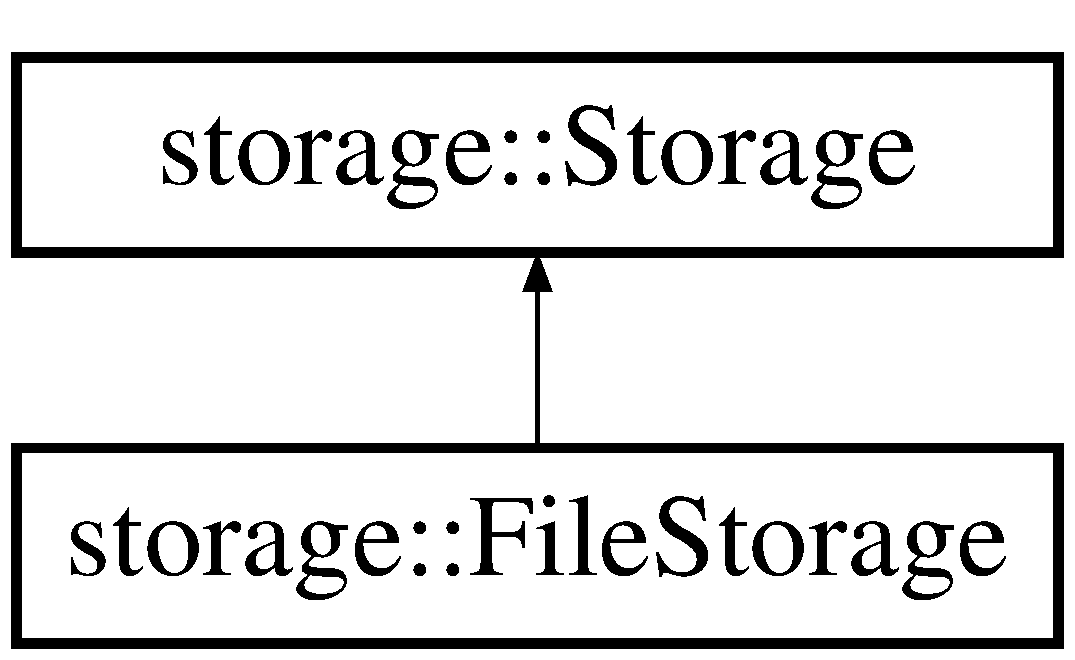
\includegraphics[height=2.000000cm]{classstorage_1_1FileStorage}
\end{center}
\end{figure}
\subsection*{\-Public \-Member \-Functions}
\begin{DoxyCompactItemize}
\item 
def \hyperlink{classstorage_1_1FileStorage_a43bd213fb32d848345a8cb7fdc34c595}{\-\_\-\-\_\-init\-\_\-\-\_\-}
\item 
def \hyperlink{classstorage_1_1FileStorage_a04e4aa0ef4c652a74825db6ab1c3dd9b}{add}
\begin{DoxyCompactList}\small\item\em \-Add a \-Task to the file storage. \end{DoxyCompactList}\item 
def \hyperlink{classstorage_1_1FileStorage_a4638796fcbe063abc5f1e43230576cae}{find}
\begin{DoxyCompactList}\small\item\em \-Return a \-Task given it's key. \end{DoxyCompactList}\item 
def \hyperlink{classstorage_1_1FileStorage_a8b2e0dbaa297155c82ed56c924674841}{get\-\_\-all}
\begin{DoxyCompactList}\small\item\em \-Return a list of all \-Tasks. \end{DoxyCompactList}\item 
def \hyperlink{classstorage_1_1FileStorage_aa14c1efcc951e67d8cd85c041e32a4bc}{update}
\begin{DoxyCompactList}\small\item\em \-Update an existing \-Task in the file storage. \end{DoxyCompactList}\item 
def \hyperlink{classstorage_1_1FileStorage_aa50ba6664b9e27d2bdcdfb4d8ce135d5}{delete}
\begin{DoxyCompactList}\small\item\em \-Delete an existing \-Task in the file storage. \end{DoxyCompactList}\item 
def \hyperlink{classstorage_1_1FileStorage_a062105b2d65e4fd3608022bb1ad3eb98}{search}
\begin{DoxyCompactList}\small\item\em \-Return a \-Task list given a search \-Task. \end{DoxyCompactList}\end{DoxyCompactItemize}
\subsection*{\-Public \-Attributes}
\begin{DoxyCompactItemize}
\item 
\hyperlink{classstorage_1_1FileStorage_a2a9a008a5ed06e3df5b5e45a3ff3d8e8}{task\-\_\-filename}
\item 
\hyperlink{classstorage_1_1FileStorage_a70122293a571deb852cdc8cf4800b0ac}{key\-\_\-filename}
\end{DoxyCompactItemize}


\subsection{\-Detailed \-Description}
\-Interface for storing \-Tasks to a file. 

\-Kwargs/\-Instance \-Vars\-: task\-\_\-filename (str)\-: \-Name of file in which to store the \-Task list. key\-\_\-filename (str)\-: \-Name of file in which to store the next key.

\-Public methods\-: add(task\-\_\-item) find(key = \-None) \hyperlink{classstorage_1_1FileStorage_a8b2e0dbaa297155c82ed56c924674841}{get\-\_\-all()} update(task\-\_\-item) delete(key) search(search\-\_\-task)

\-Reads and writes \-Task objects from a file as a single list. 

\-Definition at line 95 of file storage.\-py.



\subsection{\-Constructor \& \-Destructor \-Documentation}
\hypertarget{classstorage_1_1FileStorage_a43bd213fb32d848345a8cb7fdc34c595}{
\index{storage\-::\-File\-Storage@{storage\-::\-File\-Storage}!\-\_\-\-\_\-init\-\_\-\-\_\-@{\-\_\-\-\_\-init\-\_\-\-\_\-}}
\index{\-\_\-\-\_\-init\-\_\-\-\_\-@{\-\_\-\-\_\-init\-\_\-\-\_\-}!storage::FileStorage@{storage\-::\-File\-Storage}}
\subsubsection[{\-\_\-\-\_\-init\-\_\-\-\_\-}]{\setlength{\rightskip}{0pt plus 5cm}def storage\-::\-File\-Storage\-::\-\_\-\-\_\-init\-\_\-\-\_\- (
\begin{DoxyParamCaption}
\item[{}]{self, }
\item[{}]{task\-\_\-filename = {\ttfamily 'taskfile'}, }
\item[{}]{key\-\_\-filename = {\ttfamily 'keyfile'}}
\end{DoxyParamCaption}
)}}
\label{classstorage_1_1FileStorage_a43bd213fb32d848345a8cb7fdc34c595}


\-Definition at line 96 of file storage.\-py.



\subsection{\-Member \-Function \-Documentation}
\hypertarget{classstorage_1_1FileStorage_a04e4aa0ef4c652a74825db6ab1c3dd9b}{
\index{storage\-::\-File\-Storage@{storage\-::\-File\-Storage}!add@{add}}
\index{add@{add}!storage::FileStorage@{storage\-::\-File\-Storage}}
\subsubsection[{add}]{\setlength{\rightskip}{0pt plus 5cm}def storage\-::\-File\-Storage\-::add (
\begin{DoxyParamCaption}
\item[{}]{self, }
\item[{}]{task\-\_\-item}
\end{DoxyParamCaption}
)}}
\label{classstorage_1_1FileStorage_a04e4aa0ef4c652a74825db6ab1c3dd9b}


\-Add a \-Task to the file storage. 

\-Args\-: task\-\_\-item (\-Task)\-: \-The \-Task object to be added to storage.

\-Returns\-: task\-\_\-item.\-key (int)\-: \-Newly added \-Task's key.

\-Raises\-:

\-The \-Task object is given a key and appended to the list of \-Tasks in the file. 

\-Reimplemented from \hyperlink{classstorage_1_1Storage_abff2cc4bca8fd82e1eca9262ac6013d0}{storage\-::\-Storage}.



\-Definition at line 170 of file storage.\-py.

\hypertarget{classstorage_1_1FileStorage_aa50ba6664b9e27d2bdcdfb4d8ce135d5}{
\index{storage\-::\-File\-Storage@{storage\-::\-File\-Storage}!delete@{delete}}
\index{delete@{delete}!storage::FileStorage@{storage\-::\-File\-Storage}}
\subsubsection[{delete}]{\setlength{\rightskip}{0pt plus 5cm}def storage\-::\-File\-Storage\-::delete (
\begin{DoxyParamCaption}
\item[{}]{self, }
\item[{}]{key}
\end{DoxyParamCaption}
)}}
\label{classstorage_1_1FileStorage_aa50ba6664b9e27d2bdcdfb4d8ce135d5}


\-Delete an existing \-Task in the file storage. 

\-Args\-: key (int)\-: \-The key for the desired \-Task object to delete.

\-Returns\-: key\-\_\-match (int)\-: \-Task's key that was deleted in storage.

\-Raises\-:

\-Using the given key, iterate through the \-Task list and delete the matching \-Task. \-If none is found, nothing is deleted and return \-None. 

\-Reimplemented from \hyperlink{classstorage_1_1Storage_ab2da63e5da388a071b1a8ceccd777194}{storage\-::\-Storage}.



\-Definition at line 304 of file storage.\-py.

\hypertarget{classstorage_1_1FileStorage_a4638796fcbe063abc5f1e43230576cae}{
\index{storage\-::\-File\-Storage@{storage\-::\-File\-Storage}!find@{find}}
\index{find@{find}!storage::FileStorage@{storage\-::\-File\-Storage}}
\subsubsection[{find}]{\setlength{\rightskip}{0pt plus 5cm}def storage\-::\-File\-Storage\-::find (
\begin{DoxyParamCaption}
\item[{}]{self, }
\item[{}]{key = {\ttfamily \-None}}
\end{DoxyParamCaption}
)}}
\label{classstorage_1_1FileStorage_a4638796fcbe063abc5f1e43230576cae}


\-Return a \-Task given it's key. 

\-Args\-: key (int)\-: \-The key for the desired \-Task object.

\-Returns\-: task\-\_\-item (\-Task)\-: \-Task with matching key.

\-Raises\-:

\-Using the given key, iterate through the \-Task list and return the \-Task with matching key. \-If none is found return \-None. 

\-Reimplemented from \hyperlink{classstorage_1_1Storage_ad6eb351cfbfcc4c9dea150ce21dadcd7}{storage\-::\-Storage}.



\-Definition at line 208 of file storage.\-py.

\hypertarget{classstorage_1_1FileStorage_a8b2e0dbaa297155c82ed56c924674841}{
\index{storage\-::\-File\-Storage@{storage\-::\-File\-Storage}!get\-\_\-all@{get\-\_\-all}}
\index{get\-\_\-all@{get\-\_\-all}!storage::FileStorage@{storage\-::\-File\-Storage}}
\subsubsection[{get\-\_\-all}]{\setlength{\rightskip}{0pt plus 5cm}def storage\-::\-File\-Storage\-::get\-\_\-all (
\begin{DoxyParamCaption}
\item[{}]{self}
\end{DoxyParamCaption}
)}}
\label{classstorage_1_1FileStorage_a8b2e0dbaa297155c82ed56c924674841}


\-Return a list of all \-Tasks. 

\-Returns\-: task\-\_\-list (\-Task\mbox{[}\mbox{]})\-: \-List of every task in storage.

\-Raises\-: 

\-Reimplemented from \hyperlink{classstorage_1_1Storage_a955f60e4ddfdfa4fae84d7b6b8aad438}{storage\-::\-Storage}.



\-Definition at line 236 of file storage.\-py.

\hypertarget{classstorage_1_1FileStorage_a062105b2d65e4fd3608022bb1ad3eb98}{
\index{storage\-::\-File\-Storage@{storage\-::\-File\-Storage}!search@{search}}
\index{search@{search}!storage::FileStorage@{storage\-::\-File\-Storage}}
\subsubsection[{search}]{\setlength{\rightskip}{0pt plus 5cm}def storage\-::\-File\-Storage\-::search (
\begin{DoxyParamCaption}
\item[{}]{self, }
\item[{}]{search\-\_\-task}
\end{DoxyParamCaption}
)}}
\label{classstorage_1_1FileStorage_a062105b2d65e4fd3608022bb1ad3eb98}


\-Return a \-Task list given a search \-Task. 

\-Args\-: search\-\_\-task (\-Task)\-: \-The \-Task to be used for searching.

\-Returns\-: task\-\_\-search\-\_\-list (\-Task\mbox{[}\mbox{]})\-: \-List of \-Tasks matching search criteria.

\-Raises\-:

\-Using the given search \-Task, iterate through the \-Task list and append matching \-Tasks to a \-Task list then return this list. \-If none matches, return \-None. 

\-Reimplemented from \hyperlink{classstorage_1_1Storage_a393a72aca9a927cab5ac0a4b99d97ebb}{storage\-::\-Storage}.



\-Definition at line 342 of file storage.\-py.

\hypertarget{classstorage_1_1FileStorage_aa14c1efcc951e67d8cd85c041e32a4bc}{
\index{storage\-::\-File\-Storage@{storage\-::\-File\-Storage}!update@{update}}
\index{update@{update}!storage::FileStorage@{storage\-::\-File\-Storage}}
\subsubsection[{update}]{\setlength{\rightskip}{0pt plus 5cm}def storage\-::\-File\-Storage\-::update (
\begin{DoxyParamCaption}
\item[{}]{self, }
\item[{}]{task\-\_\-item}
\end{DoxyParamCaption}
)}}
\label{classstorage_1_1FileStorage_aa14c1efcc951e67d8cd85c041e32a4bc}


\-Update an existing \-Task in the file storage. 

\-Args\-: task\-\_\-item (\-Task)\-: \-The \-Task object to be updated.

\-Returns\-: key\-\_\-match (int)\-: \-Task's key that was updating in storage.

\-Raises\-:

\-Using the given \-Task's key, iterate through the \-Task list to find a matching key, replace the matching \-Task with the given \-Task, and return the old \-Task. \-If none is found, update nothing and return \-None. 

\-Reimplemented from \hyperlink{classstorage_1_1Storage_ae0ed2cc07e30a6f350a750c7428061e9}{storage\-::\-Storage}.



\-Definition at line 265 of file storage.\-py.



\subsection{\-Member \-Data \-Documentation}
\hypertarget{classstorage_1_1FileStorage_a70122293a571deb852cdc8cf4800b0ac}{
\index{storage\-::\-File\-Storage@{storage\-::\-File\-Storage}!key\-\_\-filename@{key\-\_\-filename}}
\index{key\-\_\-filename@{key\-\_\-filename}!storage::FileStorage@{storage\-::\-File\-Storage}}
\subsubsection[{key\-\_\-filename}]{\setlength{\rightskip}{0pt plus 5cm}{\bf storage\-::\-File\-Storage\-::key\-\_\-filename}}}
\label{classstorage_1_1FileStorage_a70122293a571deb852cdc8cf4800b0ac}


\-Definition at line 96 of file storage.\-py.

\hypertarget{classstorage_1_1FileStorage_a2a9a008a5ed06e3df5b5e45a3ff3d8e8}{
\index{storage\-::\-File\-Storage@{storage\-::\-File\-Storage}!task\-\_\-filename@{task\-\_\-filename}}
\index{task\-\_\-filename@{task\-\_\-filename}!storage::FileStorage@{storage\-::\-File\-Storage}}
\subsubsection[{task\-\_\-filename}]{\setlength{\rightskip}{0pt plus 5cm}{\bf storage\-::\-File\-Storage\-::task\-\_\-filename}}}
\label{classstorage_1_1FileStorage_a2a9a008a5ed06e3df5b5e45a3ff3d8e8}


\-Definition at line 96 of file storage.\-py.



\-The documentation for this class was generated from the following file\-:\begin{DoxyCompactItemize}
\item 
/home/scott/school/capstone/\-Task-\/\-Organizer/src/task/\hyperlink{storage_8py}{storage.\-py}\end{DoxyCompactItemize}

\hypertarget{classstorage_1_1GTaskStorage}{
\section{storage\-:\-:\-G\-Task\-Storage \-Class \-Reference}
\label{classstorage_1_1GTaskStorage}\index{storage\-::\-G\-Task\-Storage@{storage\-::\-G\-Task\-Storage}}
}


\-Interface for storing \-Tasks to \-Google \-Tasks.  


\-Inheritance diagram for storage\-:\-:\-G\-Task\-Storage\-:\begin{figure}[H]
\begin{center}
\leavevmode
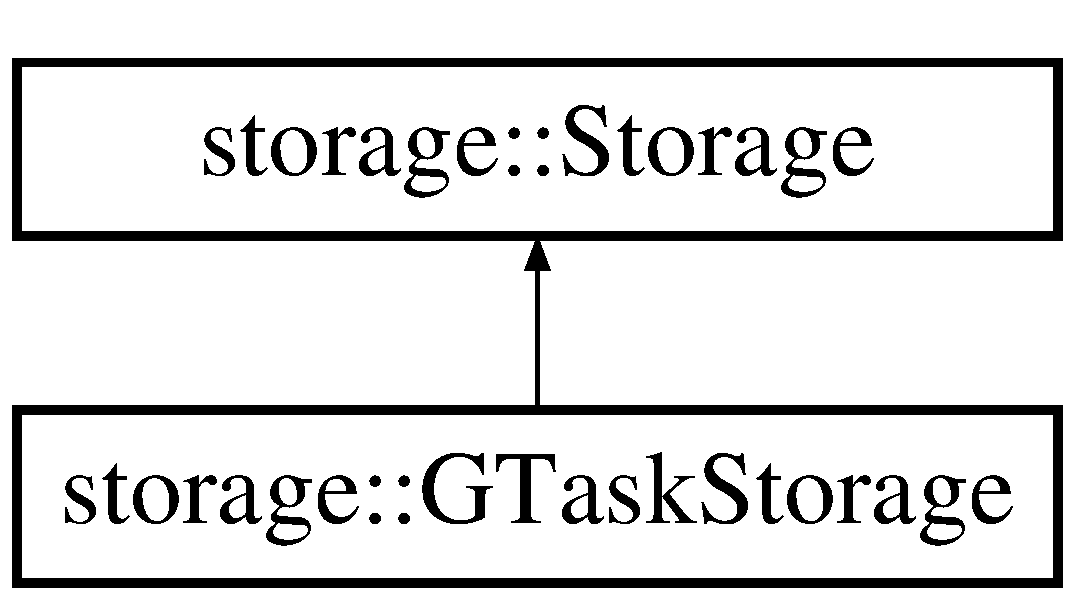
\includegraphics[height=2.000000cm]{classstorage_1_1GTaskStorage}
\end{center}
\end{figure}
\subsection*{\-Public \-Member \-Functions}
\begin{DoxyCompactItemize}
\item 
def \hyperlink{classstorage_1_1GTaskStorage_af3ffb72b776e8710e4e8b21e0332e5aa}{\-\_\-\-\_\-init\-\_\-\-\_\-}
\item 
def \hyperlink{classstorage_1_1GTaskStorage_a72ab709717d8de24f98ac7bad49e2df7}{add}
\item 
def \hyperlink{classstorage_1_1GTaskStorage_a618c0ae51a54f156dee09ecafef8d1a0}{find}
\item 
def \hyperlink{classstorage_1_1GTaskStorage_a7babf14f4d14119f9c8230d91b37ef79}{get\-\_\-all}
\item 
def \hyperlink{classstorage_1_1GTaskStorage_acc41c8c0e63a97bd2093efc542d92b1a}{update}
\item 
def \hyperlink{classstorage_1_1GTaskStorage_a6a5ecc4bf9ea5604baaf29b98d6cf311}{delete}
\item 
def \hyperlink{classstorage_1_1GTaskStorage_a1d112c05463018ea6dfa3eea65196fd6}{search}
\begin{DoxyCompactList}\small\item\em \-Return a \-Task list given a search \-Task. \end{DoxyCompactList}\end{DoxyCompactItemize}
\subsection*{\-Static \-Public \-Attributes}
\begin{DoxyCompactItemize}
\item 
\hyperlink{classstorage_1_1GTaskStorage_a587a0c1c17188d6b8d7c13866a20ba7c}{\-F\-L\-A\-G\-S} = gflags.\-F\-L\-A\-G\-S
\end{DoxyCompactItemize}


\subsection{\-Detailed \-Description}
\-Interface for storing \-Tasks to \-Google \-Tasks. 

\-Public methods\-: add(task\-\_\-item) find(key = \-None) \hyperlink{classstorage_1_1GTaskStorage_a7babf14f4d14119f9c8230d91b37ef79}{get\-\_\-all()} update(task\-\_\-item) delete(key) search(search\-\_\-task)

\-Reads and writes \-Task from \-Google \-Tasks. \-Task objects are transformed to and from \-Google's task dictionaries. 

\-Definition at line 626 of file storage.\-py.



\subsection{\-Constructor \& \-Destructor \-Documentation}
\hypertarget{classstorage_1_1GTaskStorage_af3ffb72b776e8710e4e8b21e0332e5aa}{
\index{storage\-::\-G\-Task\-Storage@{storage\-::\-G\-Task\-Storage}!\-\_\-\-\_\-init\-\_\-\-\_\-@{\-\_\-\-\_\-init\-\_\-\-\_\-}}
\index{\-\_\-\-\_\-init\-\_\-\-\_\-@{\-\_\-\-\_\-init\-\_\-\-\_\-}!storage::GTaskStorage@{storage\-::\-G\-Task\-Storage}}
\subsubsection[{\-\_\-\-\_\-init\-\_\-\-\_\-}]{\setlength{\rightskip}{0pt plus 5cm}def storage\-::\-G\-Task\-Storage\-::\-\_\-\-\_\-init\-\_\-\-\_\- (
\begin{DoxyParamCaption}
\item[{}]{self}
\end{DoxyParamCaption}
)}}
\label{classstorage_1_1GTaskStorage_af3ffb72b776e8710e4e8b21e0332e5aa}


\-Reimplemented from \hyperlink{classstorage_1_1Storage_af32106831c466787182a5363c139c849}{storage\-::\-Storage}.



\-Definition at line 629 of file storage.\-py.



\subsection{\-Member \-Function \-Documentation}
\hypertarget{classstorage_1_1GTaskStorage_a72ab709717d8de24f98ac7bad49e2df7}{
\index{storage\-::\-G\-Task\-Storage@{storage\-::\-G\-Task\-Storage}!add@{add}}
\index{add@{add}!storage::GTaskStorage@{storage\-::\-G\-Task\-Storage}}
\subsubsection[{add}]{\setlength{\rightskip}{0pt plus 5cm}def storage\-::\-G\-Task\-Storage\-::add (
\begin{DoxyParamCaption}
\item[{}]{self, }
\item[{}]{task\-\_\-item}
\end{DoxyParamCaption}
)}}
\label{classstorage_1_1GTaskStorage_a72ab709717d8de24f98ac7bad49e2df7}
\begin{DoxyVerb}Add a Task to the GTask storage.


Args:
    task_item (Task): The Task object to be added to storage.

Returns:
    task_item.key (int): Newly added Task's key.

Raises:


The Task object is added to storage and given a key.

\end{DoxyVerb}
 

\-Reimplemented from \hyperlink{classstorage_1_1Storage_abff2cc4bca8fd82e1eca9262ac6013d0}{storage\-::\-Storage}.



\-Definition at line 648 of file storage.\-py.

\hypertarget{classstorage_1_1GTaskStorage_a6a5ecc4bf9ea5604baaf29b98d6cf311}{
\index{storage\-::\-G\-Task\-Storage@{storage\-::\-G\-Task\-Storage}!delete@{delete}}
\index{delete@{delete}!storage::GTaskStorage@{storage\-::\-G\-Task\-Storage}}
\subsubsection[{delete}]{\setlength{\rightskip}{0pt plus 5cm}def storage\-::\-G\-Task\-Storage\-::delete (
\begin{DoxyParamCaption}
\item[{}]{self, }
\item[{}]{key}
\end{DoxyParamCaption}
)}}
\label{classstorage_1_1GTaskStorage_a6a5ecc4bf9ea5604baaf29b98d6cf311}
\begin{DoxyVerb}Delete an existing Task in the GTask storage.

Args:
    key (int): The key for the desired Task object to delete.

Returns:
    key_match (int): Task's key that was deleted in storage.

Raises:


Using the given key, delete the matching Task. If none is found,
nothing is deleted and return None.

\end{DoxyVerb}
 

\-Reimplemented from \hyperlink{classstorage_1_1Storage_ab2da63e5da388a071b1a8ceccd777194}{storage\-::\-Storage}.



\-Definition at line 793 of file storage.\-py.

\hypertarget{classstorage_1_1GTaskStorage_a618c0ae51a54f156dee09ecafef8d1a0}{
\index{storage\-::\-G\-Task\-Storage@{storage\-::\-G\-Task\-Storage}!find@{find}}
\index{find@{find}!storage::GTaskStorage@{storage\-::\-G\-Task\-Storage}}
\subsubsection[{find}]{\setlength{\rightskip}{0pt plus 5cm}def storage\-::\-G\-Task\-Storage\-::find (
\begin{DoxyParamCaption}
\item[{}]{self, }
\item[{}]{key = {\ttfamily \-None}}
\end{DoxyParamCaption}
)}}
\label{classstorage_1_1GTaskStorage_a618c0ae51a54f156dee09ecafef8d1a0}
\begin{DoxyVerb}Return a Task given it's key.

Args:
    key (int): The key for the desired Task object.

Returns:
    task_item (Task): Task with matching key.

Raises:


Using the given key, return the Task with the matching key. If none
is found return None.
\end{DoxyVerb}
 

\-Reimplemented from \hyperlink{classstorage_1_1Storage_ad6eb351cfbfcc4c9dea150ce21dadcd7}{storage\-::\-Storage}.



\-Definition at line 684 of file storage.\-py.

\hypertarget{classstorage_1_1GTaskStorage_a7babf14f4d14119f9c8230d91b37ef79}{
\index{storage\-::\-G\-Task\-Storage@{storage\-::\-G\-Task\-Storage}!get\-\_\-all@{get\-\_\-all}}
\index{get\-\_\-all@{get\-\_\-all}!storage::GTaskStorage@{storage\-::\-G\-Task\-Storage}}
\subsubsection[{get\-\_\-all}]{\setlength{\rightskip}{0pt plus 5cm}def storage\-::\-G\-Task\-Storage\-::get\-\_\-all (
\begin{DoxyParamCaption}
\item[{}]{self}
\end{DoxyParamCaption}
)}}
\label{classstorage_1_1GTaskStorage_a7babf14f4d14119f9c8230d91b37ef79}
\begin{DoxyVerb}Return a list of all Tasks.\end{DoxyVerb}
 

\-Reimplemented from \hyperlink{classstorage_1_1Storage_a955f60e4ddfdfa4fae84d7b6b8aad438}{storage\-::\-Storage}.



\-Definition at line 724 of file storage.\-py.

\hypertarget{classstorage_1_1GTaskStorage_a1d112c05463018ea6dfa3eea65196fd6}{
\index{storage\-::\-G\-Task\-Storage@{storage\-::\-G\-Task\-Storage}!search@{search}}
\index{search@{search}!storage::GTaskStorage@{storage\-::\-G\-Task\-Storage}}
\subsubsection[{search}]{\setlength{\rightskip}{0pt plus 5cm}def storage\-::\-G\-Task\-Storage\-::search (
\begin{DoxyParamCaption}
\item[{}]{self, }
\item[{}]{search\-\_\-task}
\end{DoxyParamCaption}
)}}
\label{classstorage_1_1GTaskStorage_a1d112c05463018ea6dfa3eea65196fd6}


\-Return a \-Task list given a search \-Task. 

\-Args\-: search\-\_\-task (\-Task)\-: \-The \-Task to be used for searching.

\-Returns\-: task\-\_\-search\-\_\-list (\-Task\mbox{[}\mbox{]})\-: \-List of \-Tasks matching search criteria.

\-Raises\-:

\-Using the given search \-Task, iterate through the \-Task list and append matching \-Tasks to a \-Task list then return this list. \-If none matches, return \-None. 

\-Reimplemented from \hyperlink{classstorage_1_1Storage_a393a72aca9a927cab5ac0a4b99d97ebb}{storage\-::\-Storage}.



\-Definition at line 845 of file storage.\-py.

\hypertarget{classstorage_1_1GTaskStorage_acc41c8c0e63a97bd2093efc542d92b1a}{
\index{storage\-::\-G\-Task\-Storage@{storage\-::\-G\-Task\-Storage}!update@{update}}
\index{update@{update}!storage::GTaskStorage@{storage\-::\-G\-Task\-Storage}}
\subsubsection[{update}]{\setlength{\rightskip}{0pt plus 5cm}def storage\-::\-G\-Task\-Storage\-::update (
\begin{DoxyParamCaption}
\item[{}]{self, }
\item[{}]{task\-\_\-item}
\end{DoxyParamCaption}
)}}
\label{classstorage_1_1GTaskStorage_acc41c8c0e63a97bd2093efc542d92b1a}
\begin{DoxyVerb}Update an existing Task in the GTask storage.

Args:
    task_item (Task): The Task object to be updated.

Returns:
    key_match (int): Task's key that was updating in storage.

Raises:


Using the given Task's key, find the Task with a matching key and
replace it with the given Task. Then return the old Task. If none
is found, updating nothing and return None.

\end{DoxyVerb}
 

\-Reimplemented from \hyperlink{classstorage_1_1Storage_ae0ed2cc07e30a6f350a750c7428061e9}{storage\-::\-Storage}.



\-Definition at line 746 of file storage.\-py.



\subsection{\-Member \-Data \-Documentation}
\hypertarget{classstorage_1_1GTaskStorage_a587a0c1c17188d6b8d7c13866a20ba7c}{
\index{storage\-::\-G\-Task\-Storage@{storage\-::\-G\-Task\-Storage}!\-F\-L\-A\-G\-S@{\-F\-L\-A\-G\-S}}
\index{\-F\-L\-A\-G\-S@{\-F\-L\-A\-G\-S}!storage::GTaskStorage@{storage\-::\-G\-Task\-Storage}}
\subsubsection[{\-F\-L\-A\-G\-S}]{\setlength{\rightskip}{0pt plus 5cm}{\bf storage\-::\-G\-Task\-Storage\-::\-F\-L\-A\-G\-S} = gflags.\-F\-L\-A\-G\-S\hspace{0.3cm}{\ttfamily  \mbox{[}static\mbox{]}}}}
\label{classstorage_1_1GTaskStorage_a587a0c1c17188d6b8d7c13866a20ba7c}


\-Definition at line 627 of file storage.\-py.



\-The documentation for this class was generated from the following file\-:\begin{DoxyCompactItemize}
\item 
/home/scott/school/capstone/\-Task-\/\-Organizer/src/task/\hyperlink{storage_8py}{storage.\-py}\end{DoxyCompactItemize}

\hypertarget{classstorage_1_1SQLiteStorage}{
\section{storage\-:\-:\-S\-Q\-Lite\-Storage \-Class \-Reference}
\label{classstorage_1_1SQLiteStorage}\index{storage\-::\-S\-Q\-Lite\-Storage@{storage\-::\-S\-Q\-Lite\-Storage}}
}


\-Interface for storing \-Tasks to a \-S\-Q\-Lite database.  


\-Inheritance diagram for storage\-:\-:\-S\-Q\-Lite\-Storage\-:\begin{figure}[H]
\begin{center}
\leavevmode
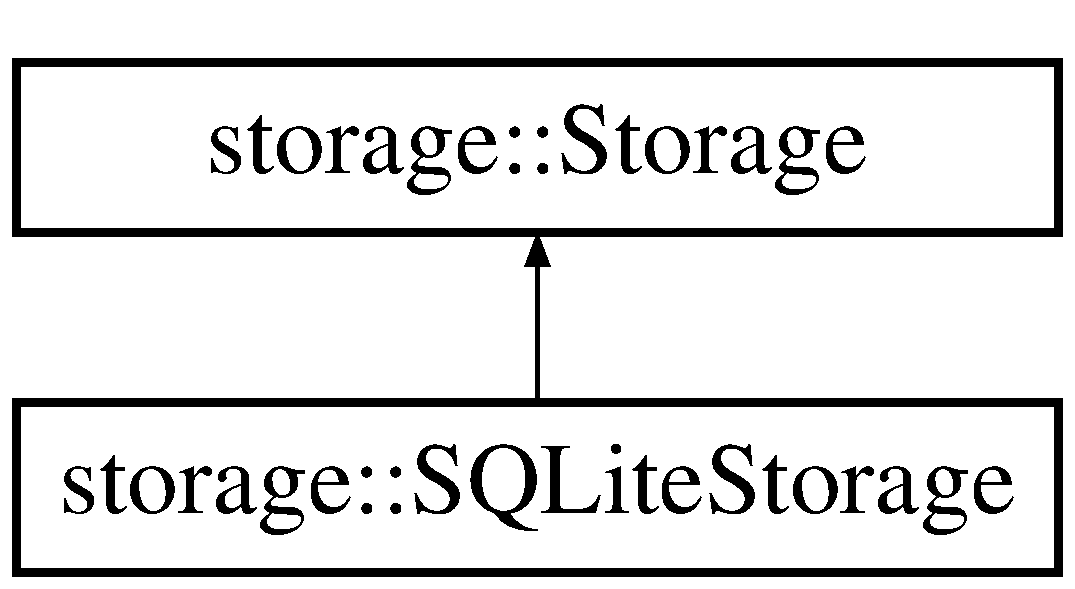
\includegraphics[height=2.000000cm]{classstorage_1_1SQLiteStorage}
\end{center}
\end{figure}
\subsection*{\-Public \-Member \-Functions}
\begin{DoxyCompactItemize}
\item 
def \hyperlink{classstorage_1_1SQLiteStorage_ac61e8f98fc1319468ec6e30b2ab9e4a7}{\-\_\-\-\_\-init\-\_\-\-\_\-}
\item 
def \hyperlink{classstorage_1_1SQLiteStorage_ae540c3c47f35a52d638f634a0782a7af}{add}
\begin{DoxyCompactList}\small\item\em \-Add a \-Task to the database storage. \end{DoxyCompactList}\item 
def \hyperlink{classstorage_1_1SQLiteStorage_a3ad42c6cfdc3a5740c461fe1a87a963a}{find}
\begin{DoxyCompactList}\small\item\em \-Return a \-Task given it's key. \end{DoxyCompactList}\item 
def \hyperlink{classstorage_1_1SQLiteStorage_a9a64b929488dfb6ceff46039a5f622ab}{get\-\_\-all}
\begin{DoxyCompactList}\small\item\em \-Return a list of all \-Task's. \end{DoxyCompactList}\item 
def \hyperlink{classstorage_1_1SQLiteStorage_a0a9ade02509f896caf7a32d02651857e}{update}
\begin{DoxyCompactList}\small\item\em \-Update an existing \-Task in the database storage. \end{DoxyCompactList}\item 
def \hyperlink{classstorage_1_1SQLiteStorage_a9ad3dc6a2fc126429be96188efda72a6}{delete}
\begin{DoxyCompactList}\small\item\em \-Delete an existing \-Task in the database storage. \end{DoxyCompactList}\item 
def \hyperlink{classstorage_1_1SQLiteStorage_a7e8c17a6ec5b2cbe72befb73bb38357c}{search}
\begin{DoxyCompactList}\small\item\em \-Return a \-Task list given a search \-Task. \end{DoxyCompactList}\end{DoxyCompactItemize}
\subsection*{\-Public \-Attributes}
\begin{DoxyCompactItemize}
\item 
\hyperlink{classstorage_1_1SQLiteStorage_a6cf1398c3b51050f89d8c3e6dab71250}{task\-\_\-dbname}
\end{DoxyCompactItemize}


\subsection{\-Detailed \-Description}
\-Interface for storing \-Tasks to a \-S\-Q\-Lite database. 

\-Kwargs/\-Instance \-Vars\-: task\-\_\-dbname (str)\-: \-Name of database/file in which to store \-Tasks.

\-Public methods\-: add(task\-\_\-item) find(key = \-None) \hyperlink{classstorage_1_1SQLiteStorage_a9a64b929488dfb6ceff46039a5f622ab}{get\-\_\-all()} update(task\-\_\-item) delete(key) search(search\-\_\-task)

\-Reads and writes \-Task objects from a sqlite database file. \-Tasks are stored in a table whos columns coincide with the \-Task's attributes. 

\-Definition at line 374 of file storage.\-py.



\subsection{\-Constructor \& \-Destructor \-Documentation}
\hypertarget{classstorage_1_1SQLiteStorage_ac61e8f98fc1319468ec6e30b2ab9e4a7}{
\index{storage\-::\-S\-Q\-Lite\-Storage@{storage\-::\-S\-Q\-Lite\-Storage}!\-\_\-\-\_\-init\-\_\-\-\_\-@{\-\_\-\-\_\-init\-\_\-\-\_\-}}
\index{\-\_\-\-\_\-init\-\_\-\-\_\-@{\-\_\-\-\_\-init\-\_\-\-\_\-}!storage::SQLiteStorage@{storage\-::\-S\-Q\-Lite\-Storage}}
\subsubsection[{\-\_\-\-\_\-init\-\_\-\-\_\-}]{\setlength{\rightskip}{0pt plus 5cm}def storage\-::\-S\-Q\-Lite\-Storage\-::\-\_\-\-\_\-init\-\_\-\-\_\- (
\begin{DoxyParamCaption}
\item[{}]{self, }
\item[{}]{task\-\_\-dbname = {\ttfamily 'taskdb'}}
\end{DoxyParamCaption}
)}}
\label{classstorage_1_1SQLiteStorage_ac61e8f98fc1319468ec6e30b2ab9e4a7}


\-Definition at line 375 of file storage.\-py.



\subsection{\-Member \-Function \-Documentation}
\hypertarget{classstorage_1_1SQLiteStorage_ae540c3c47f35a52d638f634a0782a7af}{
\index{storage\-::\-S\-Q\-Lite\-Storage@{storage\-::\-S\-Q\-Lite\-Storage}!add@{add}}
\index{add@{add}!storage::SQLiteStorage@{storage\-::\-S\-Q\-Lite\-Storage}}
\subsubsection[{add}]{\setlength{\rightskip}{0pt plus 5cm}def storage\-::\-S\-Q\-Lite\-Storage\-::add (
\begin{DoxyParamCaption}
\item[{}]{self, }
\item[{}]{task\-\_\-item}
\end{DoxyParamCaption}
)}}
\label{classstorage_1_1SQLiteStorage_ae540c3c47f35a52d638f634a0782a7af}


\-Add a \-Task to the database storage. 

\-Args\-: task\-\_\-item (\-Task)\-: \-The \-Task object to be added to storage.

\-Returns\-: task\-\_\-item.\-key (int)\-: \-Newly added \-Task's key.

\-Raises\-:

\-The \-Task object is given a key and appended to the list of \-Tasks in the database. 

\-Reimplemented from \hyperlink{classstorage_1_1Storage_abff2cc4bca8fd82e1eca9262ac6013d0}{storage\-::\-Storage}.



\-Definition at line 415 of file storage.\-py.

\hypertarget{classstorage_1_1SQLiteStorage_a9ad3dc6a2fc126429be96188efda72a6}{
\index{storage\-::\-S\-Q\-Lite\-Storage@{storage\-::\-S\-Q\-Lite\-Storage}!delete@{delete}}
\index{delete@{delete}!storage::SQLiteStorage@{storage\-::\-S\-Q\-Lite\-Storage}}
\subsubsection[{delete}]{\setlength{\rightskip}{0pt plus 5cm}def storage\-::\-S\-Q\-Lite\-Storage\-::delete (
\begin{DoxyParamCaption}
\item[{}]{self, }
\item[{}]{key}
\end{DoxyParamCaption}
)}}
\label{classstorage_1_1SQLiteStorage_a9ad3dc6a2fc126429be96188efda72a6}


\-Delete an existing \-Task in the database storage. 

\-Args\-: key (int)\-: \-The key for the desired \-Task object to delete.

\-Returns\-: key\-\_\-match (int)\-: \-Task's key that was deleted in storage.

\-Raises\-:

\-Using the given key, find the matching \-Task in the database and delete it. \-If none is found, nothing is deleted and return \-None. 

\-Reimplemented from \hyperlink{classstorage_1_1Storage_ab2da63e5da388a071b1a8ceccd777194}{storage\-::\-Storage}.



\-Definition at line 539 of file storage.\-py.

\hypertarget{classstorage_1_1SQLiteStorage_a3ad42c6cfdc3a5740c461fe1a87a963a}{
\index{storage\-::\-S\-Q\-Lite\-Storage@{storage\-::\-S\-Q\-Lite\-Storage}!find@{find}}
\index{find@{find}!storage::SQLiteStorage@{storage\-::\-S\-Q\-Lite\-Storage}}
\subsubsection[{find}]{\setlength{\rightskip}{0pt plus 5cm}def storage\-::\-S\-Q\-Lite\-Storage\-::find (
\begin{DoxyParamCaption}
\item[{}]{self, }
\item[{}]{key = {\ttfamily \-None}}
\end{DoxyParamCaption}
)}}
\label{classstorage_1_1SQLiteStorage_a3ad42c6cfdc3a5740c461fe1a87a963a}


\-Return a \-Task given it's key. 

\-Args\-: key (int)\-: \-The key for the desired \-Task object.

\-Returns\-: task\-\_\-item (\-Task)\-: \-Task with matching key.

\-Raises\-:

\-Using the given key, get the \-Task with the matching key from the database and return the \-Task. \-If none is found return \-None. 

\-Reimplemented from \hyperlink{classstorage_1_1Storage_ad6eb351cfbfcc4c9dea150ce21dadcd7}{storage\-::\-Storage}.



\-Definition at line 444 of file storage.\-py.

\hypertarget{classstorage_1_1SQLiteStorage_a9a64b929488dfb6ceff46039a5f622ab}{
\index{storage\-::\-S\-Q\-Lite\-Storage@{storage\-::\-S\-Q\-Lite\-Storage}!get\-\_\-all@{get\-\_\-all}}
\index{get\-\_\-all@{get\-\_\-all}!storage::SQLiteStorage@{storage\-::\-S\-Q\-Lite\-Storage}}
\subsubsection[{get\-\_\-all}]{\setlength{\rightskip}{0pt plus 5cm}def storage\-::\-S\-Q\-Lite\-Storage\-::get\-\_\-all (
\begin{DoxyParamCaption}
\item[{}]{self}
\end{DoxyParamCaption}
)}}
\label{classstorage_1_1SQLiteStorage_a9a64b929488dfb6ceff46039a5f622ab}


\-Return a list of all \-Task's. 



\-Reimplemented from \hyperlink{classstorage_1_1Storage_a955f60e4ddfdfa4fae84d7b6b8aad438}{storage\-::\-Storage}.



\-Definition at line 470 of file storage.\-py.

\hypertarget{classstorage_1_1SQLiteStorage_a7e8c17a6ec5b2cbe72befb73bb38357c}{
\index{storage\-::\-S\-Q\-Lite\-Storage@{storage\-::\-S\-Q\-Lite\-Storage}!search@{search}}
\index{search@{search}!storage::SQLiteStorage@{storage\-::\-S\-Q\-Lite\-Storage}}
\subsubsection[{search}]{\setlength{\rightskip}{0pt plus 5cm}def storage\-::\-S\-Q\-Lite\-Storage\-::search (
\begin{DoxyParamCaption}
\item[{}]{self, }
\item[{}]{search\-\_\-task}
\end{DoxyParamCaption}
)}}
\label{classstorage_1_1SQLiteStorage_a7e8c17a6ec5b2cbe72befb73bb38357c}


\-Return a \-Task list given a search \-Task. 

\-Args\-: search\-\_\-task (\-Task)\-: \-The \-Task to be used for searching.

\-Returns\-: task\-\_\-search\-\_\-list (\-Task\mbox{[}\mbox{]})\-: \-List of \-Tasks matching search criteria.

\-Raises\-:

\-Using the given search \-Task, return a \-Task list of all \-Tasks that match the search \-Task's attributes. 

\-Reimplemented from \hyperlink{classstorage_1_1Storage_a393a72aca9a927cab5ac0a4b99d97ebb}{storage\-::\-Storage}.



\-Definition at line 572 of file storage.\-py.

\hypertarget{classstorage_1_1SQLiteStorage_a0a9ade02509f896caf7a32d02651857e}{
\index{storage\-::\-S\-Q\-Lite\-Storage@{storage\-::\-S\-Q\-Lite\-Storage}!update@{update}}
\index{update@{update}!storage::SQLiteStorage@{storage\-::\-S\-Q\-Lite\-Storage}}
\subsubsection[{update}]{\setlength{\rightskip}{0pt plus 5cm}def storage\-::\-S\-Q\-Lite\-Storage\-::update (
\begin{DoxyParamCaption}
\item[{}]{self, }
\item[{}]{task\-\_\-item}
\end{DoxyParamCaption}
)}}
\label{classstorage_1_1SQLiteStorage_a0a9ade02509f896caf7a32d02651857e}


\-Update an existing \-Task in the database storage. 

\-Args\-: task\-\_\-item (\-Task)\-: \-The \-Task object to be updated.

\-Returns\-: key\-\_\-match (int)\-: \-Task's key that was updating in storage.

\-Raises\-:

\-Using the given \-Task's key, find the matching \-Task in the database and replace it with the given \-Task then return the old \-Task. \-If none is found, update nothing and return \-None. 

\-Reimplemented from \hyperlink{classstorage_1_1Storage_ae0ed2cc07e30a6f350a750c7428061e9}{storage\-::\-Storage}.



\-Definition at line 504 of file storage.\-py.



\subsection{\-Member \-Data \-Documentation}
\hypertarget{classstorage_1_1SQLiteStorage_a6cf1398c3b51050f89d8c3e6dab71250}{
\index{storage\-::\-S\-Q\-Lite\-Storage@{storage\-::\-S\-Q\-Lite\-Storage}!task\-\_\-dbname@{task\-\_\-dbname}}
\index{task\-\_\-dbname@{task\-\_\-dbname}!storage::SQLiteStorage@{storage\-::\-S\-Q\-Lite\-Storage}}
\subsubsection[{task\-\_\-dbname}]{\setlength{\rightskip}{0pt plus 5cm}{\bf storage\-::\-S\-Q\-Lite\-Storage\-::task\-\_\-dbname}}}
\label{classstorage_1_1SQLiteStorage_a6cf1398c3b51050f89d8c3e6dab71250}


\-Definition at line 375 of file storage.\-py.



\-The documentation for this class was generated from the following file\-:\begin{DoxyCompactItemize}
\item 
/home/scott/school/capstone/\-Task-\/\-Organizer/src/task/\hyperlink{storage_8py}{storage.\-py}\end{DoxyCompactItemize}

\hypertarget{classstorage_1_1Storage}{
\section{storage\-:\-:\-Storage \-Class \-Reference}
\label{classstorage_1_1Storage}\index{storage\-::\-Storage@{storage\-::\-Storage}}
}


\-Abstract base class for \-Task storage.  


\-Inheritance diagram for storage\-:\-:\-Storage\-:\begin{figure}[H]
\begin{center}
\leavevmode
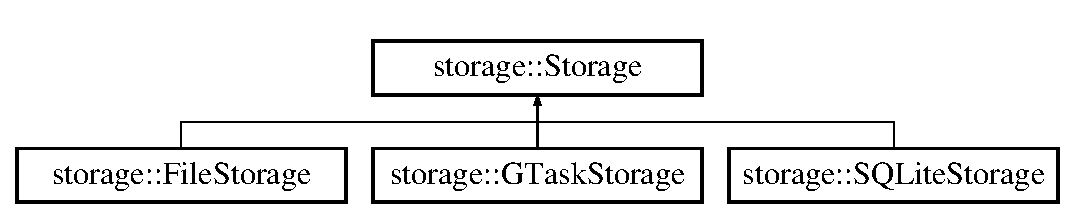
\includegraphics[height=2.000000cm]{classstorage_1_1Storage}
\end{center}
\end{figure}
\subsection*{\-Public \-Member \-Functions}
\begin{DoxyCompactItemize}
\item 
def \hyperlink{classstorage_1_1Storage_af32106831c466787182a5363c139c849}{\-\_\-\-\_\-init\-\_\-\-\_\-}
\item 
def \hyperlink{classstorage_1_1Storage_abff2cc4bca8fd82e1eca9262ac6013d0}{add}
\begin{DoxyCompactList}\small\item\em \-This functions is to be overridden by a specific storage method. \end{DoxyCompactList}\item 
def \hyperlink{classstorage_1_1Storage_ad6eb351cfbfcc4c9dea150ce21dadcd7}{find}
\begin{DoxyCompactList}\small\item\em \-This functions is to be overridden by a specific storage method. \end{DoxyCompactList}\item 
def \hyperlink{classstorage_1_1Storage_a955f60e4ddfdfa4fae84d7b6b8aad438}{get\-\_\-all}
\begin{DoxyCompactList}\small\item\em \-This functions is to be overridden by a specific storage method. \end{DoxyCompactList}\item 
def \hyperlink{classstorage_1_1Storage_ae0ed2cc07e30a6f350a750c7428061e9}{update}
\begin{DoxyCompactList}\small\item\em \-This functions is to be overridden by a specific storage method. \end{DoxyCompactList}\item 
def \hyperlink{classstorage_1_1Storage_ab2da63e5da388a071b1a8ceccd777194}{delete}
\begin{DoxyCompactList}\small\item\em \-This functions is to be overridden by a specific storage method. \end{DoxyCompactList}\item 
def \hyperlink{classstorage_1_1Storage_a393a72aca9a927cab5ac0a4b99d97ebb}{search}
\begin{DoxyCompactList}\small\item\em \-This functions is to be overridden by a specific storage method. \end{DoxyCompactList}\end{DoxyCompactItemize}


\subsection{\-Detailed \-Description}
\-Abstract base class for \-Task storage. 

\-Public methods\-: add(task\-\_\-item) find(key = \-None) \hyperlink{classstorage_1_1Storage_a955f60e4ddfdfa4fae84d7b6b8aad438}{get\-\_\-all()} update(task\-\_\-item) delete(key) search(search\-\_\-task) 

\-Definition at line 41 of file storage.\-py.



\subsection{\-Constructor \& \-Destructor \-Documentation}
\hypertarget{classstorage_1_1Storage_af32106831c466787182a5363c139c849}{
\index{storage\-::\-Storage@{storage\-::\-Storage}!\-\_\-\-\_\-init\-\_\-\-\_\-@{\-\_\-\-\_\-init\-\_\-\-\_\-}}
\index{\-\_\-\-\_\-init\-\_\-\-\_\-@{\-\_\-\-\_\-init\-\_\-\-\_\-}!storage::Storage@{storage\-::\-Storage}}
\subsubsection[{\-\_\-\-\_\-init\-\_\-\-\_\-}]{\setlength{\rightskip}{0pt plus 5cm}def storage\-::\-Storage\-::\-\_\-\-\_\-init\-\_\-\-\_\- (
\begin{DoxyParamCaption}
\item[{}]{self}
\end{DoxyParamCaption}
)}}
\label{classstorage_1_1Storage_af32106831c466787182a5363c139c849}


\-Reimplemented in \hyperlink{classstorage_1_1GTaskStorage_af3ffb72b776e8710e4e8b21e0332e5aa}{storage\-::\-G\-Task\-Storage}.



\-Definition at line 42 of file storage.\-py.



\subsection{\-Member \-Function \-Documentation}
\hypertarget{classstorage_1_1Storage_abff2cc4bca8fd82e1eca9262ac6013d0}{
\index{storage\-::\-Storage@{storage\-::\-Storage}!add@{add}}
\index{add@{add}!storage::Storage@{storage\-::\-Storage}}
\subsubsection[{add}]{\setlength{\rightskip}{0pt plus 5cm}def storage\-::\-Storage\-::add (
\begin{DoxyParamCaption}
\item[{}]{self, }
\item[{}]{task\-\_\-item}
\end{DoxyParamCaption}
)}}
\label{classstorage_1_1Storage_abff2cc4bca8fd82e1eca9262ac6013d0}


\-This functions is to be overridden by a specific storage method. 



\-Reimplemented in \hyperlink{classstorage_1_1GTaskStorage_a72ab709717d8de24f98ac7bad49e2df7}{storage\-::\-G\-Task\-Storage}, \hyperlink{classstorage_1_1SQLiteStorage_ae540c3c47f35a52d638f634a0782a7af}{storage\-::\-S\-Q\-Lite\-Storage}, and \hyperlink{classstorage_1_1FileStorage_a04e4aa0ef4c652a74825db6ab1c3dd9b}{storage\-::\-File\-Storage}.



\-Definition at line 47 of file storage.\-py.

\hypertarget{classstorage_1_1Storage_ab2da63e5da388a071b1a8ceccd777194}{
\index{storage\-::\-Storage@{storage\-::\-Storage}!delete@{delete}}
\index{delete@{delete}!storage::Storage@{storage\-::\-Storage}}
\subsubsection[{delete}]{\setlength{\rightskip}{0pt plus 5cm}def storage\-::\-Storage\-::delete (
\begin{DoxyParamCaption}
\item[{}]{self, }
\item[{}]{key}
\end{DoxyParamCaption}
)}}
\label{classstorage_1_1Storage_ab2da63e5da388a071b1a8ceccd777194}


\-This functions is to be overridden by a specific storage method. 



\-Reimplemented in \hyperlink{classstorage_1_1GTaskStorage_a6a5ecc4bf9ea5604baaf29b98d6cf311}{storage\-::\-G\-Task\-Storage}, \hyperlink{classstorage_1_1SQLiteStorage_a9ad3dc6a2fc126429be96188efda72a6}{storage\-::\-S\-Q\-Lite\-Storage}, and \hyperlink{classstorage_1_1FileStorage_aa50ba6664b9e27d2bdcdfb4d8ce135d5}{storage\-::\-File\-Storage}.



\-Definition at line 67 of file storage.\-py.

\hypertarget{classstorage_1_1Storage_ad6eb351cfbfcc4c9dea150ce21dadcd7}{
\index{storage\-::\-Storage@{storage\-::\-Storage}!find@{find}}
\index{find@{find}!storage::Storage@{storage\-::\-Storage}}
\subsubsection[{find}]{\setlength{\rightskip}{0pt plus 5cm}def storage\-::\-Storage\-::find (
\begin{DoxyParamCaption}
\item[{}]{self, }
\item[{}]{key = {\ttfamily \-None}}
\end{DoxyParamCaption}
)}}
\label{classstorage_1_1Storage_ad6eb351cfbfcc4c9dea150ce21dadcd7}


\-This functions is to be overridden by a specific storage method. 



\-Reimplemented in \hyperlink{classstorage_1_1GTaskStorage_a618c0ae51a54f156dee09ecafef8d1a0}{storage\-::\-G\-Task\-Storage}, \hyperlink{classstorage_1_1SQLiteStorage_a3ad42c6cfdc3a5740c461fe1a87a963a}{storage\-::\-S\-Q\-Lite\-Storage}, and \hyperlink{classstorage_1_1FileStorage_a4638796fcbe063abc5f1e43230576cae}{storage\-::\-File\-Storage}.



\-Definition at line 52 of file storage.\-py.

\hypertarget{classstorage_1_1Storage_a955f60e4ddfdfa4fae84d7b6b8aad438}{
\index{storage\-::\-Storage@{storage\-::\-Storage}!get\-\_\-all@{get\-\_\-all}}
\index{get\-\_\-all@{get\-\_\-all}!storage::Storage@{storage\-::\-Storage}}
\subsubsection[{get\-\_\-all}]{\setlength{\rightskip}{0pt plus 5cm}def storage\-::\-Storage\-::get\-\_\-all (
\begin{DoxyParamCaption}
\item[{}]{self}
\end{DoxyParamCaption}
)}}
\label{classstorage_1_1Storage_a955f60e4ddfdfa4fae84d7b6b8aad438}


\-This functions is to be overridden by a specific storage method. 



\-Reimplemented in \hyperlink{classstorage_1_1GTaskStorage_a7babf14f4d14119f9c8230d91b37ef79}{storage\-::\-G\-Task\-Storage}, \hyperlink{classstorage_1_1SQLiteStorage_a9a64b929488dfb6ceff46039a5f622ab}{storage\-::\-S\-Q\-Lite\-Storage}, and \hyperlink{classstorage_1_1FileStorage_a8b2e0dbaa297155c82ed56c924674841}{storage\-::\-File\-Storage}.



\-Definition at line 57 of file storage.\-py.

\hypertarget{classstorage_1_1Storage_a393a72aca9a927cab5ac0a4b99d97ebb}{
\index{storage\-::\-Storage@{storage\-::\-Storage}!search@{search}}
\index{search@{search}!storage::Storage@{storage\-::\-Storage}}
\subsubsection[{search}]{\setlength{\rightskip}{0pt plus 5cm}def storage\-::\-Storage\-::search (
\begin{DoxyParamCaption}
\item[{}]{self, }
\item[{}]{search\-\_\-task}
\end{DoxyParamCaption}
)}}
\label{classstorage_1_1Storage_a393a72aca9a927cab5ac0a4b99d97ebb}


\-This functions is to be overridden by a specific storage method. 



\-Reimplemented in \hyperlink{classstorage_1_1GTaskStorage_a1d112c05463018ea6dfa3eea65196fd6}{storage\-::\-G\-Task\-Storage}, \hyperlink{classstorage_1_1SQLiteStorage_a7e8c17a6ec5b2cbe72befb73bb38357c}{storage\-::\-S\-Q\-Lite\-Storage}, and \hyperlink{classstorage_1_1FileStorage_a062105b2d65e4fd3608022bb1ad3eb98}{storage\-::\-File\-Storage}.



\-Definition at line 72 of file storage.\-py.

\hypertarget{classstorage_1_1Storage_ae0ed2cc07e30a6f350a750c7428061e9}{
\index{storage\-::\-Storage@{storage\-::\-Storage}!update@{update}}
\index{update@{update}!storage::Storage@{storage\-::\-Storage}}
\subsubsection[{update}]{\setlength{\rightskip}{0pt plus 5cm}def storage\-::\-Storage\-::update (
\begin{DoxyParamCaption}
\item[{}]{self, }
\item[{}]{task\-\_\-item}
\end{DoxyParamCaption}
)}}
\label{classstorage_1_1Storage_ae0ed2cc07e30a6f350a750c7428061e9}


\-This functions is to be overridden by a specific storage method. 



\-Reimplemented in \hyperlink{classstorage_1_1GTaskStorage_acc41c8c0e63a97bd2093efc542d92b1a}{storage\-::\-G\-Task\-Storage}, \hyperlink{classstorage_1_1SQLiteStorage_a0a9ade02509f896caf7a32d02651857e}{storage\-::\-S\-Q\-Lite\-Storage}, and \hyperlink{classstorage_1_1FileStorage_aa14c1efcc951e67d8cd85c041e32a4bc}{storage\-::\-File\-Storage}.



\-Definition at line 62 of file storage.\-py.



\-The documentation for this class was generated from the following file\-:\begin{DoxyCompactItemize}
\item 
/home/scott/school/capstone/\-Task-\/\-Organizer/src/task/\hyperlink{storage_8py}{storage.\-py}\end{DoxyCompactItemize}

\hypertarget{classstorage_1_1StorageFactory}{
\section{storage\-:\-:\-Storage\-Factory \-Class \-Reference}
\label{classstorage_1_1StorageFactory}\index{storage\-::\-Storage\-Factory@{storage\-::\-Storage\-Factory}}
}


\-Interface for getting a storage instance.  


\subsection*{\-Public \-Member \-Functions}
\begin{DoxyCompactItemize}
\item 
def \hyperlink{classstorage_1_1StorageFactory_a5eaa9cd1a7ed0055035a6900b5413254}{\-\_\-\-\_\-init\-\_\-\-\_\-}
\item 
def \hyperlink{classstorage_1_1StorageFactory_a7b6cb77054cbecc003d88f65cfd4f664}{get}
\begin{DoxyCompactList}\small\item\em \-Return a \-Task storage instance. \end{DoxyCompactList}\end{DoxyCompactItemize}


\subsection{\-Detailed \-Description}
\-Interface for getting a storage instance. 

\-Public methods\-: get(storage\-\_\-type, kwargs)

\-Select the type of storage in which to store \-Task objects and pass arguments to the specified storage classes constructor. 

\-Definition at line 874 of file storage.\-py.



\subsection{\-Constructor \& \-Destructor \-Documentation}
\hypertarget{classstorage_1_1StorageFactory_a5eaa9cd1a7ed0055035a6900b5413254}{
\index{storage\-::\-Storage\-Factory@{storage\-::\-Storage\-Factory}!\-\_\-\-\_\-init\-\_\-\-\_\-@{\-\_\-\-\_\-init\-\_\-\-\_\-}}
\index{\-\_\-\-\_\-init\-\_\-\-\_\-@{\-\_\-\-\_\-init\-\_\-\-\_\-}!storage::StorageFactory@{storage\-::\-Storage\-Factory}}
\subsubsection[{\-\_\-\-\_\-init\-\_\-\-\_\-}]{\setlength{\rightskip}{0pt plus 5cm}def storage\-::\-Storage\-Factory\-::\-\_\-\-\_\-init\-\_\-\-\_\- (
\begin{DoxyParamCaption}
\item[{}]{self}
\end{DoxyParamCaption}
)}}
\label{classstorage_1_1StorageFactory_a5eaa9cd1a7ed0055035a6900b5413254}


\-Definition at line 875 of file storage.\-py.



\subsection{\-Member \-Function \-Documentation}
\hypertarget{classstorage_1_1StorageFactory_a7b6cb77054cbecc003d88f65cfd4f664}{
\index{storage\-::\-Storage\-Factory@{storage\-::\-Storage\-Factory}!get@{get}}
\index{get@{get}!storage::StorageFactory@{storage\-::\-Storage\-Factory}}
\subsubsection[{get}]{\setlength{\rightskip}{0pt plus 5cm}def storage\-::\-Storage\-Factory\-::get (
\begin{DoxyParamCaption}
\item[{}]{storage\-\_\-type, }
\item[{}]{kwargs}
\end{DoxyParamCaption}
)}}
\label{classstorage_1_1StorageFactory_a7b6cb77054cbecc003d88f65cfd4f664}


\-Return a \-Task storage instance. 

\-Args\-: storage\-\_\-type (str)\-: \-Name of the desired storage type. kwargs (str)\-: \-Keyword arguments specific to each storage type.

\-Returns\-: storage\-\_\-instance (\hyperlink{classstorage_1_1Storage}{\-Storage})\-: \-Child instance of a storage class.

\-Using the given storage type, create an instance with the given optional keyword arguments and return the storage instance. 

\-Definition at line 895 of file storage.\-py.



\-The documentation for this class was generated from the following file\-:\begin{DoxyCompactItemize}
\item 
/home/scott/school/capstone/\-Task-\/\-Organizer/src/task/\hyperlink{storage_8py}{storage.\-py}\end{DoxyCompactItemize}

\hypertarget{classtask_1_1Task}{
\section{task\-:\-:\-Task \-Class \-Reference}
\label{classtask_1_1Task}\index{task\-::\-Task@{task\-::\-Task}}
}


\-Instantiate a \hyperlink{classtask_1_1Task}{\-Task} object.  


\subsection*{\-Public \-Member \-Functions}
\begin{DoxyCompactItemize}
\item 
def \hyperlink{classtask_1_1Task_aa3d495c785de9774c66a730535b4c08f}{\-\_\-\-\_\-init\-\_\-\-\_\-}
\item 
def \hyperlink{classtask_1_1Task_ac32eb0d8fd34e4ae11e7cb24a1c7f99d}{\-\_\-\-\_\-str\-\_\-\-\_\-}
\item 
def \hyperlink{classtask_1_1Task_a455e3fe2cfeb638a43cbc950125af569}{\-\_\-\-\_\-eq\-\_\-\-\_\-}
\item 
def \hyperlink{classtask_1_1Task_a45fab314fc54abbc30d6c979db9b4612}{\-\_\-\-\_\-ne\-\_\-\-\_\-}
\end{DoxyCompactItemize}
\subsection*{\-Public \-Attributes}
\begin{DoxyCompactItemize}
\item 
\hyperlink{classtask_1_1Task_a028cd6524320407ce6cae1c2e4f0914a}{key}
\item 
\hyperlink{classtask_1_1Task_a877528ec8ead8e0efa64d3eb1dc0e0d1}{title}
\item 
\hyperlink{classtask_1_1Task_a4f2e0a8b798d9a631c2d32c3d53e8533}{notes}
\end{DoxyCompactItemize}


\subsection{\-Detailed \-Description}
\-Instantiate a \hyperlink{classtask_1_1Task}{\-Task} object. 

\-Provides attributes for tasks and methods to compare \hyperlink{classtask_1_1Task}{\-Task} instances. 

\-Definition at line 21 of file task.\-py.



\subsection{\-Constructor \& \-Destructor \-Documentation}
\hypertarget{classtask_1_1Task_aa3d495c785de9774c66a730535b4c08f}{
\index{task\-::\-Task@{task\-::\-Task}!\-\_\-\-\_\-init\-\_\-\-\_\-@{\-\_\-\-\_\-init\-\_\-\-\_\-}}
\index{\-\_\-\-\_\-init\-\_\-\-\_\-@{\-\_\-\-\_\-init\-\_\-\-\_\-}!task::Task@{task\-::\-Task}}
\subsubsection[{\-\_\-\-\_\-init\-\_\-\-\_\-}]{\setlength{\rightskip}{0pt plus 5cm}def task\-::\-Task\-::\-\_\-\-\_\-init\-\_\-\-\_\- (
\begin{DoxyParamCaption}
\item[{}]{self, }
\item[{}]{kwargs}
\end{DoxyParamCaption}
)}}
\label{classtask_1_1Task_aa3d495c785de9774c66a730535b4c08f}


\-Definition at line 22 of file task.\-py.



\subsection{\-Member \-Function \-Documentation}
\hypertarget{classtask_1_1Task_a455e3fe2cfeb638a43cbc950125af569}{
\index{task\-::\-Task@{task\-::\-Task}!\-\_\-\-\_\-eq\-\_\-\-\_\-@{\-\_\-\-\_\-eq\-\_\-\-\_\-}}
\index{\-\_\-\-\_\-eq\-\_\-\-\_\-@{\-\_\-\-\_\-eq\-\_\-\-\_\-}!task::Task@{task\-::\-Task}}
\subsubsection[{\-\_\-\-\_\-eq\-\_\-\-\_\-}]{\setlength{\rightskip}{0pt plus 5cm}def task\-::\-Task\-::\-\_\-\-\_\-eq\-\_\-\-\_\- (
\begin{DoxyParamCaption}
\item[{}]{self, }
\item[{}]{other}
\end{DoxyParamCaption}
)}}
\label{classtask_1_1Task_a455e3fe2cfeb638a43cbc950125af569}


\-Definition at line 52 of file task.\-py.

\hypertarget{classtask_1_1Task_a45fab314fc54abbc30d6c979db9b4612}{
\index{task\-::\-Task@{task\-::\-Task}!\-\_\-\-\_\-ne\-\_\-\-\_\-@{\-\_\-\-\_\-ne\-\_\-\-\_\-}}
\index{\-\_\-\-\_\-ne\-\_\-\-\_\-@{\-\_\-\-\_\-ne\-\_\-\-\_\-}!task::Task@{task\-::\-Task}}
\subsubsection[{\-\_\-\-\_\-ne\-\_\-\-\_\-}]{\setlength{\rightskip}{0pt plus 5cm}def task\-::\-Task\-::\-\_\-\-\_\-ne\-\_\-\-\_\- (
\begin{DoxyParamCaption}
\item[{}]{self, }
\item[{}]{other}
\end{DoxyParamCaption}
)}}
\label{classtask_1_1Task_a45fab314fc54abbc30d6c979db9b4612}


\-Definition at line 61 of file task.\-py.

\hypertarget{classtask_1_1Task_ac32eb0d8fd34e4ae11e7cb24a1c7f99d}{
\index{task\-::\-Task@{task\-::\-Task}!\-\_\-\-\_\-str\-\_\-\-\_\-@{\-\_\-\-\_\-str\-\_\-\-\_\-}}
\index{\-\_\-\-\_\-str\-\_\-\-\_\-@{\-\_\-\-\_\-str\-\_\-\-\_\-}!task::Task@{task\-::\-Task}}
\subsubsection[{\-\_\-\-\_\-str\-\_\-\-\_\-}]{\setlength{\rightskip}{0pt plus 5cm}def task\-::\-Task\-::\-\_\-\-\_\-str\-\_\-\-\_\- (
\begin{DoxyParamCaption}
\item[{}]{self}
\end{DoxyParamCaption}
)}}
\label{classtask_1_1Task_ac32eb0d8fd34e4ae11e7cb24a1c7f99d}


\-Definition at line 42 of file task.\-py.



\subsection{\-Member \-Data \-Documentation}
\hypertarget{classtask_1_1Task_a028cd6524320407ce6cae1c2e4f0914a}{
\index{task\-::\-Task@{task\-::\-Task}!key@{key}}
\index{key@{key}!task::Task@{task\-::\-Task}}
\subsubsection[{key}]{\setlength{\rightskip}{0pt plus 5cm}{\bf task\-::\-Task\-::key}}}
\label{classtask_1_1Task_a028cd6524320407ce6cae1c2e4f0914a}


\-Definition at line 22 of file task.\-py.

\hypertarget{classtask_1_1Task_a4f2e0a8b798d9a631c2d32c3d53e8533}{
\index{task\-::\-Task@{task\-::\-Task}!notes@{notes}}
\index{notes@{notes}!task::Task@{task\-::\-Task}}
\subsubsection[{notes}]{\setlength{\rightskip}{0pt plus 5cm}{\bf task\-::\-Task\-::notes}}}
\label{classtask_1_1Task_a4f2e0a8b798d9a631c2d32c3d53e8533}


\-Definition at line 22 of file task.\-py.

\hypertarget{classtask_1_1Task_a877528ec8ead8e0efa64d3eb1dc0e0d1}{
\index{task\-::\-Task@{task\-::\-Task}!title@{title}}
\index{title@{title}!task::Task@{task\-::\-Task}}
\subsubsection[{title}]{\setlength{\rightskip}{0pt plus 5cm}{\bf task\-::\-Task\-::title}}}
\label{classtask_1_1Task_a877528ec8ead8e0efa64d3eb1dc0e0d1}


\-Definition at line 22 of file task.\-py.



\-The documentation for this class was generated from the following file\-:\begin{DoxyCompactItemize}
\item 
/home/scott/school/capstone/\-Task-\/\-Organizer/src/task/\hyperlink{task_8py}{task.\-py}\end{DoxyCompactItemize}

\hypertarget{classtask_1_1TaskCreator}{
\section{task\-:\-:\-Task\-Creator \-Class \-Reference}
\label{classtask_1_1TaskCreator}\index{task\-::\-Task\-Creator@{task\-::\-Task\-Creator}}
}


\-Create a \hyperlink{classtask_1_1Task}{\-Task} instance automatically.  


\subsection*{\-Public \-Member \-Functions}
\begin{DoxyCompactItemize}
\item 
def \hyperlink{classtask_1_1TaskCreator_a2204701f72772f29e392a5ddb65cbcb2}{\-\_\-\-\_\-init\-\_\-\-\_\-}
\item 
def \hyperlink{classtask_1_1TaskCreator_a3dee0a7cebe01a4c6032270c87d76c26}{build}
\begin{DoxyCompactList}\small\item\em \-Creates a \hyperlink{classtask_1_1Task}{\-Task} instance given a dictionary. \end{DoxyCompactList}\end{DoxyCompactItemize}


\subsection{\-Detailed \-Description}
\-Create a \hyperlink{classtask_1_1Task}{\-Task} instance automatically. 

\-Public methods\-: build(arg\-\_\-dict)

\-Create a \hyperlink{classtask_1_1Task}{\-Task} instance in a automatic and safer manner. 

\-Definition at line 79 of file task.\-py.



\subsection{\-Constructor \& \-Destructor \-Documentation}
\hypertarget{classtask_1_1TaskCreator_a2204701f72772f29e392a5ddb65cbcb2}{
\index{task\-::\-Task\-Creator@{task\-::\-Task\-Creator}!\-\_\-\-\_\-init\-\_\-\-\_\-@{\-\_\-\-\_\-init\-\_\-\-\_\-}}
\index{\-\_\-\-\_\-init\-\_\-\-\_\-@{\-\_\-\-\_\-init\-\_\-\-\_\-}!task::TaskCreator@{task\-::\-Task\-Creator}}
\subsubsection[{\-\_\-\-\_\-init\-\_\-\-\_\-}]{\setlength{\rightskip}{0pt plus 5cm}def task\-::\-Task\-Creator\-::\-\_\-\-\_\-init\-\_\-\-\_\- (
\begin{DoxyParamCaption}
\item[{}]{self}
\end{DoxyParamCaption}
)}}
\label{classtask_1_1TaskCreator_a2204701f72772f29e392a5ddb65cbcb2}


\-Definition at line 80 of file task.\-py.



\subsection{\-Member \-Function \-Documentation}
\hypertarget{classtask_1_1TaskCreator_a3dee0a7cebe01a4c6032270c87d76c26}{
\index{task\-::\-Task\-Creator@{task\-::\-Task\-Creator}!build@{build}}
\index{build@{build}!task::TaskCreator@{task\-::\-Task\-Creator}}
\subsubsection[{build}]{\setlength{\rightskip}{0pt plus 5cm}def task\-::\-Task\-Creator\-::build (
\begin{DoxyParamCaption}
\item[{}]{arg\-\_\-dict}
\end{DoxyParamCaption}
)}}
\label{classtask_1_1TaskCreator_a3dee0a7cebe01a4c6032270c87d76c26}


\-Creates a \hyperlink{classtask_1_1Task}{\-Task} instance given a dictionary. 

\-Args\-: arg\-\_\-dict (dict)\-: dictionary formatted to create a \hyperlink{classtask_1_1Task}{\-Task}

\-The given dictionary must have a correct naming scheme. \-However, it can be missing any field. 

\-Definition at line 93 of file task.\-py.



\-The documentation for this class was generated from the following file\-:\begin{DoxyCompactItemize}
\item 
/home/scott/school/capstone/\-Task-\/\-Organizer/src/task/\hyperlink{task_8py}{task.\-py}\end{DoxyCompactItemize}

\hypertarget{classtest__ctask_1_1TestCTask}{
\section{test\-\_\-ctask\-:\-:\-Test\-C\-Task \-Class \-Reference}
\label{classtest__ctask_1_1TestCTask}\index{test\-\_\-ctask\-::\-Test\-C\-Task@{test\-\_\-ctask\-::\-Test\-C\-Task}}
}


\-Tests parsing of the command line for the ctask script.  


\subsection*{\-Public \-Member \-Functions}
\begin{DoxyCompactItemize}
\item 
def \hyperlink{classtest__ctask_1_1TestCTask_ac2b990e80afb15bc40b3ce737596a1d3}{set\-Up}
\item 
def \hyperlink{classtest__ctask_1_1TestCTask_a3130d849eedea4a6473e38bd3b26c572}{tear\-Down}
\item 
def \hyperlink{classtest__ctask_1_1TestCTask_a9417196e5f2414a02d8a90e8f28ca517}{test\-\_\-add\-\_\-subparser}
\begin{DoxyCompactList}\small\item\em \-Tests the parser when the add sub-\/command is specified. \end{DoxyCompactList}\item 
def \hyperlink{classtest__ctask_1_1TestCTask_a4599d2f1c1d3ab69ff08a1481cea15d9}{test\-\_\-find\-\_\-subparser}
\begin{DoxyCompactList}\small\item\em \-Tests the parser when the find sub-\/command is specified. \end{DoxyCompactList}\item 
def \hyperlink{classtest__ctask_1_1TestCTask_ad6d78332e27eb6b7ee1c7100296a8800}{test\-\_\-edit\-\_\-subparser}
\begin{DoxyCompactList}\small\item\em \-Tests the parser when the edit sub-\/command is specified. \end{DoxyCompactList}\item 
def \hyperlink{classtest__ctask_1_1TestCTask_a8499a5d20427be6f0fe8876753a14acb}{test\-\_\-delete\-\_\-subparser}
\begin{DoxyCompactList}\small\item\em \-Tests the parser when the del sub-\/command is specified. \end{DoxyCompactList}\item 
def \hyperlink{classtest__ctask_1_1TestCTask_aba1a6e0e712bb178fc717a0f909a4a09}{test\-\_\-parse\-\_\-cl\-\_\-args}
\begin{DoxyCompactList}\small\item\em \-Tests that options are correctly transformed into a dict. \end{DoxyCompactList}\end{DoxyCompactItemize}
\subsection*{\-Public \-Attributes}
\begin{DoxyCompactItemize}
\item 
\hyperlink{classtest__ctask_1_1TestCTask_a4a4548da4574705418d96e0810ddb26e}{test\-\_\-task\-\_\-filename}
\item 
\hyperlink{classtest__ctask_1_1TestCTask_ad52e6d91453657dc773f0a5bf5fe6b28}{test\-\_\-key\-\_\-filename}
\item 
\hyperlink{classtest__ctask_1_1TestCTask_ad45378108691bb4812431e6c7697249e}{parser}
\item 
\hyperlink{classtest__ctask_1_1TestCTask_aae958d2cb8adb03d0f568a8bef5ccc82}{title}
\item 
\hyperlink{classtest__ctask_1_1TestCTask_a82df515fe85cae2ad1851572e96cd956}{notes}
\item 
\hyperlink{classtest__ctask_1_1TestCTask_ae31553d1f4d94741e4cc95ea1866b977}{key}
\end{DoxyCompactItemize}


\subsection{\-Detailed \-Description}
\-Tests parsing of the command line for the ctask script. 



\-Definition at line 10 of file test\-\_\-ctask.\-py.



\subsection{\-Member \-Function \-Documentation}
\hypertarget{classtest__ctask_1_1TestCTask_ac2b990e80afb15bc40b3ce737596a1d3}{
\index{test\-\_\-ctask\-::\-Test\-C\-Task@{test\-\_\-ctask\-::\-Test\-C\-Task}!set\-Up@{set\-Up}}
\index{set\-Up@{set\-Up}!test_ctask::TestCTask@{test\-\_\-ctask\-::\-Test\-C\-Task}}
\subsubsection[{set\-Up}]{\setlength{\rightskip}{0pt plus 5cm}def test\-\_\-ctask\-::\-Test\-C\-Task\-::set\-Up (
\begin{DoxyParamCaption}
\item[{}]{self}
\end{DoxyParamCaption}
)}}
\label{classtest__ctask_1_1TestCTask_ac2b990e80afb15bc40b3ce737596a1d3}


\-Definition at line 12 of file test\-\_\-ctask.\-py.

\hypertarget{classtest__ctask_1_1TestCTask_a3130d849eedea4a6473e38bd3b26c572}{
\index{test\-\_\-ctask\-::\-Test\-C\-Task@{test\-\_\-ctask\-::\-Test\-C\-Task}!tear\-Down@{tear\-Down}}
\index{tear\-Down@{tear\-Down}!test_ctask::TestCTask@{test\-\_\-ctask\-::\-Test\-C\-Task}}
\subsubsection[{tear\-Down}]{\setlength{\rightskip}{0pt plus 5cm}def test\-\_\-ctask\-::\-Test\-C\-Task\-::tear\-Down (
\begin{DoxyParamCaption}
\item[{}]{self}
\end{DoxyParamCaption}
)}}
\label{classtest__ctask_1_1TestCTask_a3130d849eedea4a6473e38bd3b26c572}


\-Definition at line 26 of file test\-\_\-ctask.\-py.

\hypertarget{classtest__ctask_1_1TestCTask_a9417196e5f2414a02d8a90e8f28ca517}{
\index{test\-\_\-ctask\-::\-Test\-C\-Task@{test\-\_\-ctask\-::\-Test\-C\-Task}!test\-\_\-add\-\_\-subparser@{test\-\_\-add\-\_\-subparser}}
\index{test\-\_\-add\-\_\-subparser@{test\-\_\-add\-\_\-subparser}!test_ctask::TestCTask@{test\-\_\-ctask\-::\-Test\-C\-Task}}
\subsubsection[{test\-\_\-add\-\_\-subparser}]{\setlength{\rightskip}{0pt plus 5cm}def test\-\_\-ctask\-::\-Test\-C\-Task\-::test\-\_\-add\-\_\-subparser (
\begin{DoxyParamCaption}
\item[{}]{self}
\end{DoxyParamCaption}
)}}
\label{classtest__ctask_1_1TestCTask_a9417196e5f2414a02d8a90e8f28ca517}


\-Tests the parser when the add sub-\/command is specified. 



\-Definition at line 32 of file test\-\_\-ctask.\-py.

\hypertarget{classtest__ctask_1_1TestCTask_a8499a5d20427be6f0fe8876753a14acb}{
\index{test\-\_\-ctask\-::\-Test\-C\-Task@{test\-\_\-ctask\-::\-Test\-C\-Task}!test\-\_\-delete\-\_\-subparser@{test\-\_\-delete\-\_\-subparser}}
\index{test\-\_\-delete\-\_\-subparser@{test\-\_\-delete\-\_\-subparser}!test_ctask::TestCTask@{test\-\_\-ctask\-::\-Test\-C\-Task}}
\subsubsection[{test\-\_\-delete\-\_\-subparser}]{\setlength{\rightskip}{0pt plus 5cm}def test\-\_\-ctask\-::\-Test\-C\-Task\-::test\-\_\-delete\-\_\-subparser (
\begin{DoxyParamCaption}
\item[{}]{self}
\end{DoxyParamCaption}
)}}
\label{classtest__ctask_1_1TestCTask_a8499a5d20427be6f0fe8876753a14acb}


\-Tests the parser when the del sub-\/command is specified. 



\-Definition at line 78 of file test\-\_\-ctask.\-py.

\hypertarget{classtest__ctask_1_1TestCTask_ad6d78332e27eb6b7ee1c7100296a8800}{
\index{test\-\_\-ctask\-::\-Test\-C\-Task@{test\-\_\-ctask\-::\-Test\-C\-Task}!test\-\_\-edit\-\_\-subparser@{test\-\_\-edit\-\_\-subparser}}
\index{test\-\_\-edit\-\_\-subparser@{test\-\_\-edit\-\_\-subparser}!test_ctask::TestCTask@{test\-\_\-ctask\-::\-Test\-C\-Task}}
\subsubsection[{test\-\_\-edit\-\_\-subparser}]{\setlength{\rightskip}{0pt plus 5cm}def test\-\_\-ctask\-::\-Test\-C\-Task\-::test\-\_\-edit\-\_\-subparser (
\begin{DoxyParamCaption}
\item[{}]{self}
\end{DoxyParamCaption}
)}}
\label{classtest__ctask_1_1TestCTask_ad6d78332e27eb6b7ee1c7100296a8800}


\-Tests the parser when the edit sub-\/command is specified. 



\-Definition at line 62 of file test\-\_\-ctask.\-py.

\hypertarget{classtest__ctask_1_1TestCTask_a4599d2f1c1d3ab69ff08a1481cea15d9}{
\index{test\-\_\-ctask\-::\-Test\-C\-Task@{test\-\_\-ctask\-::\-Test\-C\-Task}!test\-\_\-find\-\_\-subparser@{test\-\_\-find\-\_\-subparser}}
\index{test\-\_\-find\-\_\-subparser@{test\-\_\-find\-\_\-subparser}!test_ctask::TestCTask@{test\-\_\-ctask\-::\-Test\-C\-Task}}
\subsubsection[{test\-\_\-find\-\_\-subparser}]{\setlength{\rightskip}{0pt plus 5cm}def test\-\_\-ctask\-::\-Test\-C\-Task\-::test\-\_\-find\-\_\-subparser (
\begin{DoxyParamCaption}
\item[{}]{self}
\end{DoxyParamCaption}
)}}
\label{classtest__ctask_1_1TestCTask_a4599d2f1c1d3ab69ff08a1481cea15d9}


\-Tests the parser when the find sub-\/command is specified. 



\-Definition at line 48 of file test\-\_\-ctask.\-py.

\hypertarget{classtest__ctask_1_1TestCTask_aba1a6e0e712bb178fc717a0f909a4a09}{
\index{test\-\_\-ctask\-::\-Test\-C\-Task@{test\-\_\-ctask\-::\-Test\-C\-Task}!test\-\_\-parse\-\_\-cl\-\_\-args@{test\-\_\-parse\-\_\-cl\-\_\-args}}
\index{test\-\_\-parse\-\_\-cl\-\_\-args@{test\-\_\-parse\-\_\-cl\-\_\-args}!test_ctask::TestCTask@{test\-\_\-ctask\-::\-Test\-C\-Task}}
\subsubsection[{test\-\_\-parse\-\_\-cl\-\_\-args}]{\setlength{\rightskip}{0pt plus 5cm}def test\-\_\-ctask\-::\-Test\-C\-Task\-::test\-\_\-parse\-\_\-cl\-\_\-args (
\begin{DoxyParamCaption}
\item[{}]{self}
\end{DoxyParamCaption}
)}}
\label{classtest__ctask_1_1TestCTask_aba1a6e0e712bb178fc717a0f909a4a09}


\-Tests that options are correctly transformed into a dict. 



\-Definition at line 92 of file test\-\_\-ctask.\-py.



\subsection{\-Member \-Data \-Documentation}
\hypertarget{classtest__ctask_1_1TestCTask_ae31553d1f4d94741e4cc95ea1866b977}{
\index{test\-\_\-ctask\-::\-Test\-C\-Task@{test\-\_\-ctask\-::\-Test\-C\-Task}!key@{key}}
\index{key@{key}!test_ctask::TestCTask@{test\-\_\-ctask\-::\-Test\-C\-Task}}
\subsubsection[{key}]{\setlength{\rightskip}{0pt plus 5cm}{\bf test\-\_\-ctask\-::\-Test\-C\-Task\-::key}}}
\label{classtest__ctask_1_1TestCTask_ae31553d1f4d94741e4cc95ea1866b977}


\-Definition at line 12 of file test\-\_\-ctask.\-py.

\hypertarget{classtest__ctask_1_1TestCTask_a82df515fe85cae2ad1851572e96cd956}{
\index{test\-\_\-ctask\-::\-Test\-C\-Task@{test\-\_\-ctask\-::\-Test\-C\-Task}!notes@{notes}}
\index{notes@{notes}!test_ctask::TestCTask@{test\-\_\-ctask\-::\-Test\-C\-Task}}
\subsubsection[{notes}]{\setlength{\rightskip}{0pt plus 5cm}{\bf test\-\_\-ctask\-::\-Test\-C\-Task\-::notes}}}
\label{classtest__ctask_1_1TestCTask_a82df515fe85cae2ad1851572e96cd956}


\-Definition at line 12 of file test\-\_\-ctask.\-py.

\hypertarget{classtest__ctask_1_1TestCTask_ad45378108691bb4812431e6c7697249e}{
\index{test\-\_\-ctask\-::\-Test\-C\-Task@{test\-\_\-ctask\-::\-Test\-C\-Task}!parser@{parser}}
\index{parser@{parser}!test_ctask::TestCTask@{test\-\_\-ctask\-::\-Test\-C\-Task}}
\subsubsection[{parser}]{\setlength{\rightskip}{0pt plus 5cm}{\bf test\-\_\-ctask\-::\-Test\-C\-Task\-::parser}}}
\label{classtest__ctask_1_1TestCTask_ad45378108691bb4812431e6c7697249e}


\-Definition at line 12 of file test\-\_\-ctask.\-py.

\hypertarget{classtest__ctask_1_1TestCTask_ad52e6d91453657dc773f0a5bf5fe6b28}{
\index{test\-\_\-ctask\-::\-Test\-C\-Task@{test\-\_\-ctask\-::\-Test\-C\-Task}!test\-\_\-key\-\_\-filename@{test\-\_\-key\-\_\-filename}}
\index{test\-\_\-key\-\_\-filename@{test\-\_\-key\-\_\-filename}!test_ctask::TestCTask@{test\-\_\-ctask\-::\-Test\-C\-Task}}
\subsubsection[{test\-\_\-key\-\_\-filename}]{\setlength{\rightskip}{0pt plus 5cm}{\bf test\-\_\-ctask\-::\-Test\-C\-Task\-::test\-\_\-key\-\_\-filename}}}
\label{classtest__ctask_1_1TestCTask_ad52e6d91453657dc773f0a5bf5fe6b28}


\-Definition at line 12 of file test\-\_\-ctask.\-py.

\hypertarget{classtest__ctask_1_1TestCTask_a4a4548da4574705418d96e0810ddb26e}{
\index{test\-\_\-ctask\-::\-Test\-C\-Task@{test\-\_\-ctask\-::\-Test\-C\-Task}!test\-\_\-task\-\_\-filename@{test\-\_\-task\-\_\-filename}}
\index{test\-\_\-task\-\_\-filename@{test\-\_\-task\-\_\-filename}!test_ctask::TestCTask@{test\-\_\-ctask\-::\-Test\-C\-Task}}
\subsubsection[{test\-\_\-task\-\_\-filename}]{\setlength{\rightskip}{0pt plus 5cm}{\bf test\-\_\-ctask\-::\-Test\-C\-Task\-::test\-\_\-task\-\_\-filename}}}
\label{classtest__ctask_1_1TestCTask_a4a4548da4574705418d96e0810ddb26e}


\-Definition at line 12 of file test\-\_\-ctask.\-py.

\hypertarget{classtest__ctask_1_1TestCTask_aae958d2cb8adb03d0f568a8bef5ccc82}{
\index{test\-\_\-ctask\-::\-Test\-C\-Task@{test\-\_\-ctask\-::\-Test\-C\-Task}!title@{title}}
\index{title@{title}!test_ctask::TestCTask@{test\-\_\-ctask\-::\-Test\-C\-Task}}
\subsubsection[{title}]{\setlength{\rightskip}{0pt plus 5cm}{\bf test\-\_\-ctask\-::\-Test\-C\-Task\-::title}}}
\label{classtest__ctask_1_1TestCTask_aae958d2cb8adb03d0f568a8bef5ccc82}


\-Definition at line 12 of file test\-\_\-ctask.\-py.



\-The documentation for this class was generated from the following file\-:\begin{DoxyCompactItemize}
\item 
/home/scott/school/capstone/\-Task-\/\-Organizer/src/test/\hyperlink{test__ctask_8py}{test\-\_\-ctask.\-py}\end{DoxyCompactItemize}

\hypertarget{classtest__taskstorage_1_1TestFileStorage}{
\section{test\-\_\-taskstorage\-:\-:\-Test\-File\-Storage \-Class \-Reference}
\label{classtest__taskstorage_1_1TestFileStorage}\index{test\-\_\-taskstorage\-::\-Test\-File\-Storage@{test\-\_\-taskstorage\-::\-Test\-File\-Storage}}
}


\-Tests specific to the \-File\-Storage class.  


\-Inheritance diagram for test\-\_\-taskstorage\-:\-:\-Test\-File\-Storage\-:\begin{figure}[H]
\begin{center}
\leavevmode
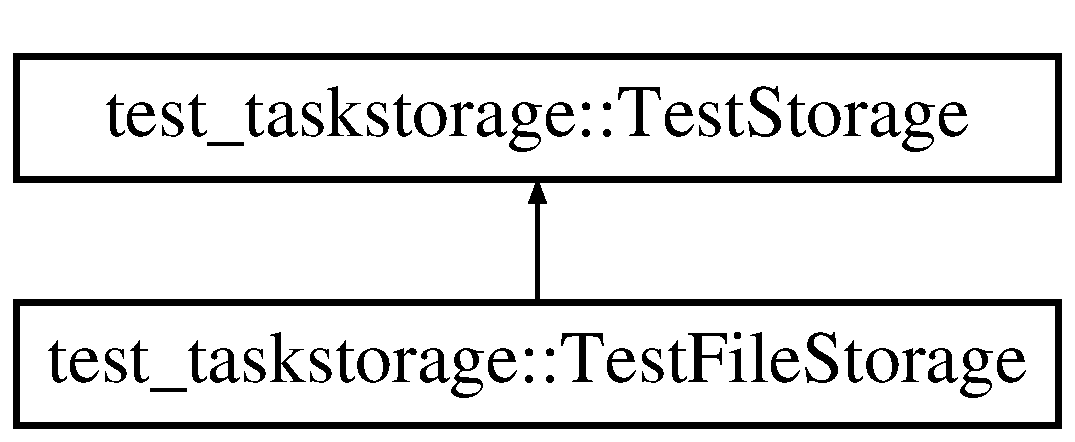
\includegraphics[height=2.000000cm]{classtest__taskstorage_1_1TestFileStorage}
\end{center}
\end{figure}
\subsection*{\-Public \-Member \-Functions}
\begin{DoxyCompactItemize}
\item 
def \hyperlink{classtest__taskstorage_1_1TestFileStorage_a3aeeb19983b93f40da74ca6f741bca7b}{\-\_\-\-\_\-init\-\_\-\-\_\-}
\item 
def \hyperlink{classtest__taskstorage_1_1TestFileStorage_adf1f62f0b4f514585227479a35c2518d}{set\-Up}
\item 
def \hyperlink{classtest__taskstorage_1_1TestFileStorage_a2c10eb94b9fa8f243eabdc40331195e1}{tear\-Down}
\item 
def \hyperlink{classtest__taskstorage_1_1TestFileStorage_a94f3a21c9b66c5351712e79942526f25}{test\-\_\-add\-\_\-read\-\_\-fail}
\begin{DoxyCompactList}\small\item\em \-Tests add()'s handling of failed file reading. \end{DoxyCompactList}\item 
def \hyperlink{classtest__taskstorage_1_1TestFileStorage_a577f8c7ca1fb81d18062761d609113a6}{test\-\_\-add\-\_\-write\-\_\-fail}
\begin{DoxyCompactList}\small\item\em \-Tests add()'s handling of failed file writing. \end{DoxyCompactList}\item 
def \hyperlink{classtest__taskstorage_1_1TestFileStorage_a14e1c7da85f39ebc27eeb51bf443447b}{test\-\_\-find\-\_\-read\-\_\-fail}
\begin{DoxyCompactList}\small\item\em \-Tests find()'s handling of failed file reading. \end{DoxyCompactList}\item 
def \hyperlink{classtest__taskstorage_1_1TestFileStorage_aff0b0b77c268949c05df2a26679e7600}{test\-\_\-get\-\_\-all\-\_\-read\-\_\-fail}
\begin{DoxyCompactList}\small\item\em \-Tests get\-\_\-all()'s handling of failed file reading. \end{DoxyCompactList}\item 
def \hyperlink{classtest__taskstorage_1_1TestFileStorage_aa5f6b47510be7afc5644fe0960a2306d}{test\-\_\-update\-\_\-write\-\_\-fail}
\begin{DoxyCompactList}\small\item\em \-Tests update()'s handling of failed file writing. \end{DoxyCompactList}\item 
def \hyperlink{classtest__taskstorage_1_1TestFileStorage_a3abac0acbf03cf24f4b73ea6bf2ba57e}{test\-\_\-delete\-\_\-write\-\_\-fail}
\begin{DoxyCompactList}\small\item\em \-Tests delete()'s handling of failed file writing. \end{DoxyCompactList}\end{DoxyCompactItemize}
\subsection*{\-Public \-Attributes}
\begin{DoxyCompactItemize}
\item 
\hyperlink{classtest__taskstorage_1_1TestFileStorage_a986e73f6663aa98ee3f90e1be3fa2515}{my\-\_\-task}
\item 
\hyperlink{classtest__taskstorage_1_1TestFileStorage_a15bcd037e6610f37504c88b03b72db5a}{test\-\_\-task\-\_\-filename}
\item 
\hyperlink{classtest__taskstorage_1_1TestFileStorage_a81c2f46a258898fea8b1bd41dfe8c896}{test\-\_\-key\-\_\-filename}
\item 
\hyperlink{classtest__taskstorage_1_1TestFileStorage_af65fc75e8b921b475ea610cf3681e270}{task\-\_\-storage}
\end{DoxyCompactItemize}


\subsection{\-Detailed \-Description}
\-Tests specific to the \-File\-Storage class. 

\-Tests that only apply to the implementation of the \-File\-Storage class and not other task\-\_\-storage types. 

\-Definition at line 169 of file test\-\_\-taskstorage.\-py.



\subsection{\-Constructor \& \-Destructor \-Documentation}
\hypertarget{classtest__taskstorage_1_1TestFileStorage_a3aeeb19983b93f40da74ca6f741bca7b}{
\index{test\-\_\-taskstorage\-::\-Test\-File\-Storage@{test\-\_\-taskstorage\-::\-Test\-File\-Storage}!\-\_\-\-\_\-init\-\_\-\-\_\-@{\-\_\-\-\_\-init\-\_\-\-\_\-}}
\index{\-\_\-\-\_\-init\-\_\-\-\_\-@{\-\_\-\-\_\-init\-\_\-\-\_\-}!test_taskstorage::TestFileStorage@{test\-\_\-taskstorage\-::\-Test\-File\-Storage}}
\subsubsection[{\-\_\-\-\_\-init\-\_\-\-\_\-}]{\setlength{\rightskip}{0pt plus 5cm}def test\-\_\-taskstorage\-::\-Test\-File\-Storage\-::\-\_\-\-\_\-init\-\_\-\-\_\- (
\begin{DoxyParamCaption}
\item[{}]{self, }
\item[{}]{method\-\_\-name}
\end{DoxyParamCaption}
)}}
\label{classtest__taskstorage_1_1TestFileStorage_a3aeeb19983b93f40da74ca6f741bca7b}


\-Reimplemented from \hyperlink{classtest__taskstorage_1_1TestStorage_a41a9bc77946b61981cdaebb9cdff74f8}{test\-\_\-taskstorage\-::\-Test\-Storage}.



\-Definition at line 171 of file test\-\_\-taskstorage.\-py.



\subsection{\-Member \-Function \-Documentation}
\hypertarget{classtest__taskstorage_1_1TestFileStorage_adf1f62f0b4f514585227479a35c2518d}{
\index{test\-\_\-taskstorage\-::\-Test\-File\-Storage@{test\-\_\-taskstorage\-::\-Test\-File\-Storage}!set\-Up@{set\-Up}}
\index{set\-Up@{set\-Up}!test_taskstorage::TestFileStorage@{test\-\_\-taskstorage\-::\-Test\-File\-Storage}}
\subsubsection[{set\-Up}]{\setlength{\rightskip}{0pt plus 5cm}def test\-\_\-taskstorage\-::\-Test\-File\-Storage\-::set\-Up (
\begin{DoxyParamCaption}
\item[{}]{self}
\end{DoxyParamCaption}
)}}
\label{classtest__taskstorage_1_1TestFileStorage_adf1f62f0b4f514585227479a35c2518d}


\-Definition at line 174 of file test\-\_\-taskstorage.\-py.

\hypertarget{classtest__taskstorage_1_1TestFileStorage_a2c10eb94b9fa8f243eabdc40331195e1}{
\index{test\-\_\-taskstorage\-::\-Test\-File\-Storage@{test\-\_\-taskstorage\-::\-Test\-File\-Storage}!tear\-Down@{tear\-Down}}
\index{tear\-Down@{tear\-Down}!test_taskstorage::TestFileStorage@{test\-\_\-taskstorage\-::\-Test\-File\-Storage}}
\subsubsection[{tear\-Down}]{\setlength{\rightskip}{0pt plus 5cm}def test\-\_\-taskstorage\-::\-Test\-File\-Storage\-::tear\-Down (
\begin{DoxyParamCaption}
\item[{}]{self}
\end{DoxyParamCaption}
)}}
\label{classtest__taskstorage_1_1TestFileStorage_a2c10eb94b9fa8f243eabdc40331195e1}


\-Definition at line 190 of file test\-\_\-taskstorage.\-py.

\hypertarget{classtest__taskstorage_1_1TestFileStorage_a94f3a21c9b66c5351712e79942526f25}{
\index{test\-\_\-taskstorage\-::\-Test\-File\-Storage@{test\-\_\-taskstorage\-::\-Test\-File\-Storage}!test\-\_\-add\-\_\-read\-\_\-fail@{test\-\_\-add\-\_\-read\-\_\-fail}}
\index{test\-\_\-add\-\_\-read\-\_\-fail@{test\-\_\-add\-\_\-read\-\_\-fail}!test_taskstorage::TestFileStorage@{test\-\_\-taskstorage\-::\-Test\-File\-Storage}}
\subsubsection[{test\-\_\-add\-\_\-read\-\_\-fail}]{\setlength{\rightskip}{0pt plus 5cm}def test\-\_\-taskstorage\-::\-Test\-File\-Storage\-::test\-\_\-add\-\_\-read\-\_\-fail (
\begin{DoxyParamCaption}
\item[{}]{self}
\end{DoxyParamCaption}
)}}
\label{classtest__taskstorage_1_1TestFileStorage_a94f3a21c9b66c5351712e79942526f25}


\-Tests add()'s handling of failed file reading. 



\-Definition at line 200 of file test\-\_\-taskstorage.\-py.

\hypertarget{classtest__taskstorage_1_1TestFileStorage_a577f8c7ca1fb81d18062761d609113a6}{
\index{test\-\_\-taskstorage\-::\-Test\-File\-Storage@{test\-\_\-taskstorage\-::\-Test\-File\-Storage}!test\-\_\-add\-\_\-write\-\_\-fail@{test\-\_\-add\-\_\-write\-\_\-fail}}
\index{test\-\_\-add\-\_\-write\-\_\-fail@{test\-\_\-add\-\_\-write\-\_\-fail}!test_taskstorage::TestFileStorage@{test\-\_\-taskstorage\-::\-Test\-File\-Storage}}
\subsubsection[{test\-\_\-add\-\_\-write\-\_\-fail}]{\setlength{\rightskip}{0pt plus 5cm}def test\-\_\-taskstorage\-::\-Test\-File\-Storage\-::test\-\_\-add\-\_\-write\-\_\-fail (
\begin{DoxyParamCaption}
\item[{}]{self}
\end{DoxyParamCaption}
)}}
\label{classtest__taskstorage_1_1TestFileStorage_a577f8c7ca1fb81d18062761d609113a6}


\-Tests add()'s handling of failed file writing. 



\-Definition at line 210 of file test\-\_\-taskstorage.\-py.

\hypertarget{classtest__taskstorage_1_1TestFileStorage_a3abac0acbf03cf24f4b73ea6bf2ba57e}{
\index{test\-\_\-taskstorage\-::\-Test\-File\-Storage@{test\-\_\-taskstorage\-::\-Test\-File\-Storage}!test\-\_\-delete\-\_\-write\-\_\-fail@{test\-\_\-delete\-\_\-write\-\_\-fail}}
\index{test\-\_\-delete\-\_\-write\-\_\-fail@{test\-\_\-delete\-\_\-write\-\_\-fail}!test_taskstorage::TestFileStorage@{test\-\_\-taskstorage\-::\-Test\-File\-Storage}}
\subsubsection[{test\-\_\-delete\-\_\-write\-\_\-fail}]{\setlength{\rightskip}{0pt plus 5cm}def test\-\_\-taskstorage\-::\-Test\-File\-Storage\-::test\-\_\-delete\-\_\-write\-\_\-fail (
\begin{DoxyParamCaption}
\item[{}]{self}
\end{DoxyParamCaption}
)}}
\label{classtest__taskstorage_1_1TestFileStorage_a3abac0acbf03cf24f4b73ea6bf2ba57e}


\-Tests delete()'s handling of failed file writing. 



\-Definition at line 245 of file test\-\_\-taskstorage.\-py.

\hypertarget{classtest__taskstorage_1_1TestFileStorage_a14e1c7da85f39ebc27eeb51bf443447b}{
\index{test\-\_\-taskstorage\-::\-Test\-File\-Storage@{test\-\_\-taskstorage\-::\-Test\-File\-Storage}!test\-\_\-find\-\_\-read\-\_\-fail@{test\-\_\-find\-\_\-read\-\_\-fail}}
\index{test\-\_\-find\-\_\-read\-\_\-fail@{test\-\_\-find\-\_\-read\-\_\-fail}!test_taskstorage::TestFileStorage@{test\-\_\-taskstorage\-::\-Test\-File\-Storage}}
\subsubsection[{test\-\_\-find\-\_\-read\-\_\-fail}]{\setlength{\rightskip}{0pt plus 5cm}def test\-\_\-taskstorage\-::\-Test\-File\-Storage\-::test\-\_\-find\-\_\-read\-\_\-fail (
\begin{DoxyParamCaption}
\item[{}]{self}
\end{DoxyParamCaption}
)}}
\label{classtest__taskstorage_1_1TestFileStorage_a14e1c7da85f39ebc27eeb51bf443447b}


\-Tests find()'s handling of failed file reading. 



\-Definition at line 217 of file test\-\_\-taskstorage.\-py.

\hypertarget{classtest__taskstorage_1_1TestFileStorage_aff0b0b77c268949c05df2a26679e7600}{
\index{test\-\_\-taskstorage\-::\-Test\-File\-Storage@{test\-\_\-taskstorage\-::\-Test\-File\-Storage}!test\-\_\-get\-\_\-all\-\_\-read\-\_\-fail@{test\-\_\-get\-\_\-all\-\_\-read\-\_\-fail}}
\index{test\-\_\-get\-\_\-all\-\_\-read\-\_\-fail@{test\-\_\-get\-\_\-all\-\_\-read\-\_\-fail}!test_taskstorage::TestFileStorage@{test\-\_\-taskstorage\-::\-Test\-File\-Storage}}
\subsubsection[{test\-\_\-get\-\_\-all\-\_\-read\-\_\-fail}]{\setlength{\rightskip}{0pt plus 5cm}def test\-\_\-taskstorage\-::\-Test\-File\-Storage\-::test\-\_\-get\-\_\-all\-\_\-read\-\_\-fail (
\begin{DoxyParamCaption}
\item[{}]{self}
\end{DoxyParamCaption}
)}}
\label{classtest__taskstorage_1_1TestFileStorage_aff0b0b77c268949c05df2a26679e7600}


\-Tests get\-\_\-all()'s handling of failed file reading. 



\-Definition at line 227 of file test\-\_\-taskstorage.\-py.

\hypertarget{classtest__taskstorage_1_1TestFileStorage_aa5f6b47510be7afc5644fe0960a2306d}{
\index{test\-\_\-taskstorage\-::\-Test\-File\-Storage@{test\-\_\-taskstorage\-::\-Test\-File\-Storage}!test\-\_\-update\-\_\-write\-\_\-fail@{test\-\_\-update\-\_\-write\-\_\-fail}}
\index{test\-\_\-update\-\_\-write\-\_\-fail@{test\-\_\-update\-\_\-write\-\_\-fail}!test_taskstorage::TestFileStorage@{test\-\_\-taskstorage\-::\-Test\-File\-Storage}}
\subsubsection[{test\-\_\-update\-\_\-write\-\_\-fail}]{\setlength{\rightskip}{0pt plus 5cm}def test\-\_\-taskstorage\-::\-Test\-File\-Storage\-::test\-\_\-update\-\_\-write\-\_\-fail (
\begin{DoxyParamCaption}
\item[{}]{self}
\end{DoxyParamCaption}
)}}
\label{classtest__taskstorage_1_1TestFileStorage_aa5f6b47510be7afc5644fe0960a2306d}


\-Tests update()'s handling of failed file writing. 



\-Definition at line 237 of file test\-\_\-taskstorage.\-py.



\subsection{\-Member \-Data \-Documentation}
\hypertarget{classtest__taskstorage_1_1TestFileStorage_a986e73f6663aa98ee3f90e1be3fa2515}{
\index{test\-\_\-taskstorage\-::\-Test\-File\-Storage@{test\-\_\-taskstorage\-::\-Test\-File\-Storage}!my\-\_\-task@{my\-\_\-task}}
\index{my\-\_\-task@{my\-\_\-task}!test_taskstorage::TestFileStorage@{test\-\_\-taskstorage\-::\-Test\-File\-Storage}}
\subsubsection[{my\-\_\-task}]{\setlength{\rightskip}{0pt plus 5cm}{\bf test\-\_\-taskstorage\-::\-Test\-File\-Storage\-::my\-\_\-task}}}
\label{classtest__taskstorage_1_1TestFileStorage_a986e73f6663aa98ee3f90e1be3fa2515}


\-Reimplemented from \hyperlink{classtest__taskstorage_1_1TestStorage_a7d47cd41a51cd29b6f793d373599bd82}{test\-\_\-taskstorage\-::\-Test\-Storage}.



\-Definition at line 174 of file test\-\_\-taskstorage.\-py.

\hypertarget{classtest__taskstorage_1_1TestFileStorage_af65fc75e8b921b475ea610cf3681e270}{
\index{test\-\_\-taskstorage\-::\-Test\-File\-Storage@{test\-\_\-taskstorage\-::\-Test\-File\-Storage}!task\-\_\-storage@{task\-\_\-storage}}
\index{task\-\_\-storage@{task\-\_\-storage}!test_taskstorage::TestFileStorage@{test\-\_\-taskstorage\-::\-Test\-File\-Storage}}
\subsubsection[{task\-\_\-storage}]{\setlength{\rightskip}{0pt plus 5cm}{\bf test\-\_\-taskstorage\-::\-Test\-File\-Storage\-::task\-\_\-storage}}}
\label{classtest__taskstorage_1_1TestFileStorage_af65fc75e8b921b475ea610cf3681e270}


\-Reimplemented from \hyperlink{classtest__taskstorage_1_1TestStorage_a414fec77c1f9ac66b58f26df514fc048}{test\-\_\-taskstorage\-::\-Test\-Storage}.



\-Definition at line 174 of file test\-\_\-taskstorage.\-py.

\hypertarget{classtest__taskstorage_1_1TestFileStorage_a81c2f46a258898fea8b1bd41dfe8c896}{
\index{test\-\_\-taskstorage\-::\-Test\-File\-Storage@{test\-\_\-taskstorage\-::\-Test\-File\-Storage}!test\-\_\-key\-\_\-filename@{test\-\_\-key\-\_\-filename}}
\index{test\-\_\-key\-\_\-filename@{test\-\_\-key\-\_\-filename}!test_taskstorage::TestFileStorage@{test\-\_\-taskstorage\-::\-Test\-File\-Storage}}
\subsubsection[{test\-\_\-key\-\_\-filename}]{\setlength{\rightskip}{0pt plus 5cm}{\bf test\-\_\-taskstorage\-::\-Test\-File\-Storage\-::test\-\_\-key\-\_\-filename}}}
\label{classtest__taskstorage_1_1TestFileStorage_a81c2f46a258898fea8b1bd41dfe8c896}


\-Definition at line 174 of file test\-\_\-taskstorage.\-py.

\hypertarget{classtest__taskstorage_1_1TestFileStorage_a15bcd037e6610f37504c88b03b72db5a}{
\index{test\-\_\-taskstorage\-::\-Test\-File\-Storage@{test\-\_\-taskstorage\-::\-Test\-File\-Storage}!test\-\_\-task\-\_\-filename@{test\-\_\-task\-\_\-filename}}
\index{test\-\_\-task\-\_\-filename@{test\-\_\-task\-\_\-filename}!test_taskstorage::TestFileStorage@{test\-\_\-taskstorage\-::\-Test\-File\-Storage}}
\subsubsection[{test\-\_\-task\-\_\-filename}]{\setlength{\rightskip}{0pt plus 5cm}{\bf test\-\_\-taskstorage\-::\-Test\-File\-Storage\-::test\-\_\-task\-\_\-filename}}}
\label{classtest__taskstorage_1_1TestFileStorage_a15bcd037e6610f37504c88b03b72db5a}


\-Definition at line 174 of file test\-\_\-taskstorage.\-py.



\-The documentation for this class was generated from the following file\-:\begin{DoxyCompactItemize}
\item 
/home/scott/school/capstone/\-Task-\/\-Organizer/src/test/\hyperlink{test__taskstorage_8py}{test\-\_\-taskstorage.\-py}\end{DoxyCompactItemize}

\hypertarget{classtest__taskstorage_1_1TestGenericStorage}{
\section{test\-\_\-taskstorage\-:\-:\-Test\-Generic\-Storage \-Class \-Reference}
\label{classtest__taskstorage_1_1TestGenericStorage}\index{test\-\_\-taskstorage\-::\-Test\-Generic\-Storage@{test\-\_\-taskstorage\-::\-Test\-Generic\-Storage}}
}


\-Tests the \-Storage abstract base class directly.  


\subsection*{\-Public \-Member \-Functions}
\begin{DoxyCompactItemize}
\item 
def \hyperlink{classtest__taskstorage_1_1TestGenericStorage_a64b019d0c45401c0a5d5bba7c8af279f}{set\-Up}
\item 
def \hyperlink{classtest__taskstorage_1_1TestGenericStorage_a4d9fdf15f42f17d40e594ba615a7d1aa}{tear\-Down}
\item 
def \hyperlink{classtest__taskstorage_1_1TestGenericStorage_ac5ba583c94f300d11eac69962a72003b}{test\-\_\-not\-\_\-implemented}
\begin{DoxyCompactList}\small\item\em \-Tests error handling in storage's abstract functions. \end{DoxyCompactList}\end{DoxyCompactItemize}
\subsection*{\-Public \-Attributes}
\begin{DoxyCompactItemize}
\item 
\hyperlink{classtest__taskstorage_1_1TestGenericStorage_a8ab0dfe56db3b3522240af6aa43de0d2}{my\-\_\-task}
\item 
\hyperlink{classtest__taskstorage_1_1TestGenericStorage_ac596a1ade6c8e90762704557da93d4bd}{storage\-\_\-instance}
\end{DoxyCompactItemize}


\subsection{\-Detailed \-Description}
\-Tests the \-Storage abstract base class directly. 

\-Tests that \-Storage abstract base class handles direct instantiations. 

\-Definition at line 123 of file test\-\_\-taskstorage.\-py.



\subsection{\-Member \-Function \-Documentation}
\hypertarget{classtest__taskstorage_1_1TestGenericStorage_a64b019d0c45401c0a5d5bba7c8af279f}{
\index{test\-\_\-taskstorage\-::\-Test\-Generic\-Storage@{test\-\_\-taskstorage\-::\-Test\-Generic\-Storage}!set\-Up@{set\-Up}}
\index{set\-Up@{set\-Up}!test_taskstorage::TestGenericStorage@{test\-\_\-taskstorage\-::\-Test\-Generic\-Storage}}
\subsubsection[{set\-Up}]{\setlength{\rightskip}{0pt plus 5cm}def test\-\_\-taskstorage\-::\-Test\-Generic\-Storage\-::set\-Up (
\begin{DoxyParamCaption}
\item[{}]{self}
\end{DoxyParamCaption}
)}}
\label{classtest__taskstorage_1_1TestGenericStorage_a64b019d0c45401c0a5d5bba7c8af279f}


\-Definition at line 125 of file test\-\_\-taskstorage.\-py.

\hypertarget{classtest__taskstorage_1_1TestGenericStorage_a4d9fdf15f42f17d40e594ba615a7d1aa}{
\index{test\-\_\-taskstorage\-::\-Test\-Generic\-Storage@{test\-\_\-taskstorage\-::\-Test\-Generic\-Storage}!tear\-Down@{tear\-Down}}
\index{tear\-Down@{tear\-Down}!test_taskstorage::TestGenericStorage@{test\-\_\-taskstorage\-::\-Test\-Generic\-Storage}}
\subsubsection[{tear\-Down}]{\setlength{\rightskip}{0pt plus 5cm}def test\-\_\-taskstorage\-::\-Test\-Generic\-Storage\-::tear\-Down (
\begin{DoxyParamCaption}
\item[{}]{self}
\end{DoxyParamCaption}
)}}
\label{classtest__taskstorage_1_1TestGenericStorage_a4d9fdf15f42f17d40e594ba615a7d1aa}


\-Definition at line 129 of file test\-\_\-taskstorage.\-py.

\hypertarget{classtest__taskstorage_1_1TestGenericStorage_ac5ba583c94f300d11eac69962a72003b}{
\index{test\-\_\-taskstorage\-::\-Test\-Generic\-Storage@{test\-\_\-taskstorage\-::\-Test\-Generic\-Storage}!test\-\_\-not\-\_\-implemented@{test\-\_\-not\-\_\-implemented}}
\index{test\-\_\-not\-\_\-implemented@{test\-\_\-not\-\_\-implemented}!test_taskstorage::TestGenericStorage@{test\-\_\-taskstorage\-::\-Test\-Generic\-Storage}}
\subsubsection[{test\-\_\-not\-\_\-implemented}]{\setlength{\rightskip}{0pt plus 5cm}def test\-\_\-taskstorage\-::\-Test\-Generic\-Storage\-::test\-\_\-not\-\_\-implemented (
\begin{DoxyParamCaption}
\item[{}]{self}
\end{DoxyParamCaption}
)}}
\label{classtest__taskstorage_1_1TestGenericStorage_ac5ba583c94f300d11eac69962a72003b}


\-Tests error handling in storage's abstract functions. 



\-Definition at line 134 of file test\-\_\-taskstorage.\-py.



\subsection{\-Member \-Data \-Documentation}
\hypertarget{classtest__taskstorage_1_1TestGenericStorage_a8ab0dfe56db3b3522240af6aa43de0d2}{
\index{test\-\_\-taskstorage\-::\-Test\-Generic\-Storage@{test\-\_\-taskstorage\-::\-Test\-Generic\-Storage}!my\-\_\-task@{my\-\_\-task}}
\index{my\-\_\-task@{my\-\_\-task}!test_taskstorage::TestGenericStorage@{test\-\_\-taskstorage\-::\-Test\-Generic\-Storage}}
\subsubsection[{my\-\_\-task}]{\setlength{\rightskip}{0pt plus 5cm}{\bf test\-\_\-taskstorage\-::\-Test\-Generic\-Storage\-::my\-\_\-task}}}
\label{classtest__taskstorage_1_1TestGenericStorage_a8ab0dfe56db3b3522240af6aa43de0d2}


\-Definition at line 125 of file test\-\_\-taskstorage.\-py.

\hypertarget{classtest__taskstorage_1_1TestGenericStorage_ac596a1ade6c8e90762704557da93d4bd}{
\index{test\-\_\-taskstorage\-::\-Test\-Generic\-Storage@{test\-\_\-taskstorage\-::\-Test\-Generic\-Storage}!storage\-\_\-instance@{storage\-\_\-instance}}
\index{storage\-\_\-instance@{storage\-\_\-instance}!test_taskstorage::TestGenericStorage@{test\-\_\-taskstorage\-::\-Test\-Generic\-Storage}}
\subsubsection[{storage\-\_\-instance}]{\setlength{\rightskip}{0pt plus 5cm}{\bf test\-\_\-taskstorage\-::\-Test\-Generic\-Storage\-::storage\-\_\-instance}}}
\label{classtest__taskstorage_1_1TestGenericStorage_ac596a1ade6c8e90762704557da93d4bd}


\-Definition at line 125 of file test\-\_\-taskstorage.\-py.



\-The documentation for this class was generated from the following file\-:\begin{DoxyCompactItemize}
\item 
/home/scott/school/capstone/\-Task-\/\-Organizer/src/test/\hyperlink{test__taskstorage_8py}{test\-\_\-taskstorage.\-py}\end{DoxyCompactItemize}

\hypertarget{classtest__taskstorage_1_1TestGTaskStorage}{
\section{test\-\_\-taskstorage\-:\-:\-Test\-G\-Task\-Storage \-Class \-Reference}
\label{classtest__taskstorage_1_1TestGTaskStorage}\index{test\-\_\-taskstorage\-::\-Test\-G\-Task\-Storage@{test\-\_\-taskstorage\-::\-Test\-G\-Task\-Storage}}
}


\-Tests specific to the \-G\-Task\-Storage class.  


\-Inheritance diagram for test\-\_\-taskstorage\-:\-:\-Test\-G\-Task\-Storage\-:\begin{figure}[H]
\begin{center}
\leavevmode
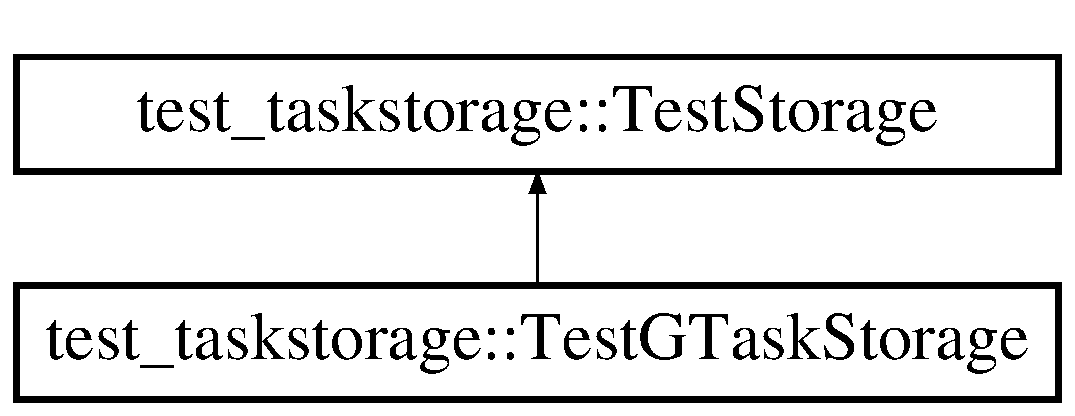
\includegraphics[height=2.000000cm]{classtest__taskstorage_1_1TestGTaskStorage}
\end{center}
\end{figure}
\subsection*{\-Public \-Member \-Functions}
\begin{DoxyCompactItemize}
\item 
def \hyperlink{classtest__taskstorage_1_1TestGTaskStorage_ae5d725daa8804f4bf01b56a5ba28303f}{\-\_\-\-\_\-init\-\_\-\-\_\-}
\item 
def \hyperlink{classtest__taskstorage_1_1TestGTaskStorage_a95893244013933d0bbcc94470b1f560b}{set\-Up}
\item 
def \hyperlink{classtest__taskstorage_1_1TestGTaskStorage_a5611e72f932b66811a0a17939ba65189}{tear\-Down}
\item 
def \hyperlink{classtest__taskstorage_1_1TestGTaskStorage_a8ee10a8d67c0d362ea2665bac82c2646}{test\-\_\-update\-\_\-no\-\_\-note}
\begin{DoxyCompactList}\small\item\em \-Tests that update() acts correctly when no note is specified. \end{DoxyCompactList}\end{DoxyCompactItemize}
\subsection*{\-Public \-Attributes}
\begin{DoxyCompactItemize}
\item 
\hyperlink{classtest__taskstorage_1_1TestGTaskStorage_a64044ab25309aa17502a40daa5983923}{my\-\_\-task}
\item 
\hyperlink{classtest__taskstorage_1_1TestGTaskStorage_abb748de83f5fdbc145f7570464fe13b7}{task\-\_\-storage}
\end{DoxyCompactItemize}


\subsection{\-Detailed \-Description}
\-Tests specific to the \-G\-Task\-Storage class. 

\-Tests that only apply to the implementation of the \-G\-Task\-Storage class and not other task\-\_\-storage types. 

\-Definition at line 297 of file test\-\_\-taskstorage.\-py.



\subsection{\-Constructor \& \-Destructor \-Documentation}
\hypertarget{classtest__taskstorage_1_1TestGTaskStorage_ae5d725daa8804f4bf01b56a5ba28303f}{
\index{test\-\_\-taskstorage\-::\-Test\-G\-Task\-Storage@{test\-\_\-taskstorage\-::\-Test\-G\-Task\-Storage}!\-\_\-\-\_\-init\-\_\-\-\_\-@{\-\_\-\-\_\-init\-\_\-\-\_\-}}
\index{\-\_\-\-\_\-init\-\_\-\-\_\-@{\-\_\-\-\_\-init\-\_\-\-\_\-}!test_taskstorage::TestGTaskStorage@{test\-\_\-taskstorage\-::\-Test\-G\-Task\-Storage}}
\subsubsection[{\-\_\-\-\_\-init\-\_\-\-\_\-}]{\setlength{\rightskip}{0pt plus 5cm}def test\-\_\-taskstorage\-::\-Test\-G\-Task\-Storage\-::\-\_\-\-\_\-init\-\_\-\-\_\- (
\begin{DoxyParamCaption}
\item[{}]{self, }
\item[{}]{method\-\_\-name}
\end{DoxyParamCaption}
)}}
\label{classtest__taskstorage_1_1TestGTaskStorage_ae5d725daa8804f4bf01b56a5ba28303f}


\-Reimplemented from \hyperlink{classtest__taskstorage_1_1TestStorage_a41a9bc77946b61981cdaebb9cdff74f8}{test\-\_\-taskstorage\-::\-Test\-Storage}.



\-Definition at line 299 of file test\-\_\-taskstorage.\-py.



\subsection{\-Member \-Function \-Documentation}
\hypertarget{classtest__taskstorage_1_1TestGTaskStorage_a95893244013933d0bbcc94470b1f560b}{
\index{test\-\_\-taskstorage\-::\-Test\-G\-Task\-Storage@{test\-\_\-taskstorage\-::\-Test\-G\-Task\-Storage}!set\-Up@{set\-Up}}
\index{set\-Up@{set\-Up}!test_taskstorage::TestGTaskStorage@{test\-\_\-taskstorage\-::\-Test\-G\-Task\-Storage}}
\subsubsection[{set\-Up}]{\setlength{\rightskip}{0pt plus 5cm}def test\-\_\-taskstorage\-::\-Test\-G\-Task\-Storage\-::set\-Up (
\begin{DoxyParamCaption}
\item[{}]{self}
\end{DoxyParamCaption}
)}}
\label{classtest__taskstorage_1_1TestGTaskStorage_a95893244013933d0bbcc94470b1f560b}


\-Definition at line 302 of file test\-\_\-taskstorage.\-py.

\hypertarget{classtest__taskstorage_1_1TestGTaskStorage_a5611e72f932b66811a0a17939ba65189}{
\index{test\-\_\-taskstorage\-::\-Test\-G\-Task\-Storage@{test\-\_\-taskstorage\-::\-Test\-G\-Task\-Storage}!tear\-Down@{tear\-Down}}
\index{tear\-Down@{tear\-Down}!test_taskstorage::TestGTaskStorage@{test\-\_\-taskstorage\-::\-Test\-G\-Task\-Storage}}
\subsubsection[{tear\-Down}]{\setlength{\rightskip}{0pt plus 5cm}def test\-\_\-taskstorage\-::\-Test\-G\-Task\-Storage\-::tear\-Down (
\begin{DoxyParamCaption}
\item[{}]{self}
\end{DoxyParamCaption}
)}}
\label{classtest__taskstorage_1_1TestGTaskStorage_a5611e72f932b66811a0a17939ba65189}


\-Definition at line 311 of file test\-\_\-taskstorage.\-py.

\hypertarget{classtest__taskstorage_1_1TestGTaskStorage_a8ee10a8d67c0d362ea2665bac82c2646}{
\index{test\-\_\-taskstorage\-::\-Test\-G\-Task\-Storage@{test\-\_\-taskstorage\-::\-Test\-G\-Task\-Storage}!test\-\_\-update\-\_\-no\-\_\-note@{test\-\_\-update\-\_\-no\-\_\-note}}
\index{test\-\_\-update\-\_\-no\-\_\-note@{test\-\_\-update\-\_\-no\-\_\-note}!test_taskstorage::TestGTaskStorage@{test\-\_\-taskstorage\-::\-Test\-G\-Task\-Storage}}
\subsubsection[{test\-\_\-update\-\_\-no\-\_\-note}]{\setlength{\rightskip}{0pt plus 5cm}def test\-\_\-taskstorage\-::\-Test\-G\-Task\-Storage\-::test\-\_\-update\-\_\-no\-\_\-note (
\begin{DoxyParamCaption}
\item[{}]{self}
\end{DoxyParamCaption}
)}}
\label{classtest__taskstorage_1_1TestGTaskStorage_a8ee10a8d67c0d362ea2665bac82c2646}


\-Tests that update() acts correctly when no note is specified. 



\-Definition at line 319 of file test\-\_\-taskstorage.\-py.



\subsection{\-Member \-Data \-Documentation}
\hypertarget{classtest__taskstorage_1_1TestGTaskStorage_a64044ab25309aa17502a40daa5983923}{
\index{test\-\_\-taskstorage\-::\-Test\-G\-Task\-Storage@{test\-\_\-taskstorage\-::\-Test\-G\-Task\-Storage}!my\-\_\-task@{my\-\_\-task}}
\index{my\-\_\-task@{my\-\_\-task}!test_taskstorage::TestGTaskStorage@{test\-\_\-taskstorage\-::\-Test\-G\-Task\-Storage}}
\subsubsection[{my\-\_\-task}]{\setlength{\rightskip}{0pt plus 5cm}{\bf test\-\_\-taskstorage\-::\-Test\-G\-Task\-Storage\-::my\-\_\-task}}}
\label{classtest__taskstorage_1_1TestGTaskStorage_a64044ab25309aa17502a40daa5983923}


\-Reimplemented from \hyperlink{classtest__taskstorage_1_1TestStorage_a7d47cd41a51cd29b6f793d373599bd82}{test\-\_\-taskstorage\-::\-Test\-Storage}.



\-Definition at line 302 of file test\-\_\-taskstorage.\-py.

\hypertarget{classtest__taskstorage_1_1TestGTaskStorage_abb748de83f5fdbc145f7570464fe13b7}{
\index{test\-\_\-taskstorage\-::\-Test\-G\-Task\-Storage@{test\-\_\-taskstorage\-::\-Test\-G\-Task\-Storage}!task\-\_\-storage@{task\-\_\-storage}}
\index{task\-\_\-storage@{task\-\_\-storage}!test_taskstorage::TestGTaskStorage@{test\-\_\-taskstorage\-::\-Test\-G\-Task\-Storage}}
\subsubsection[{task\-\_\-storage}]{\setlength{\rightskip}{0pt plus 5cm}{\bf test\-\_\-taskstorage\-::\-Test\-G\-Task\-Storage\-::task\-\_\-storage}}}
\label{classtest__taskstorage_1_1TestGTaskStorage_abb748de83f5fdbc145f7570464fe13b7}


\-Reimplemented from \hyperlink{classtest__taskstorage_1_1TestStorage_a414fec77c1f9ac66b58f26df514fc048}{test\-\_\-taskstorage\-::\-Test\-Storage}.



\-Definition at line 302 of file test\-\_\-taskstorage.\-py.



\-The documentation for this class was generated from the following file\-:\begin{DoxyCompactItemize}
\item 
/home/scott/school/capstone/\-Task-\/\-Organizer/src/test/\hyperlink{test__taskstorage_8py}{test\-\_\-taskstorage.\-py}\end{DoxyCompactItemize}

\hypertarget{classtest__taskstorage_1_1TestKeyGenerator}{
\section{test\-\_\-taskstorage\-:\-:\-Test\-Key\-Generator \-Class \-Reference}
\label{classtest__taskstorage_1_1TestKeyGenerator}\index{test\-\_\-taskstorage\-::\-Test\-Key\-Generator@{test\-\_\-taskstorage\-::\-Test\-Key\-Generator}}
}


\-Tests for the \-Key\-Generator class.  


\subsection*{\-Public \-Member \-Functions}
\begin{DoxyCompactItemize}
\item 
def \hyperlink{classtest__taskstorage_1_1TestKeyGenerator_a533dcdf1f1da6ba47e7262cd2126297a}{set\-Up}
\item 
def \hyperlink{classtest__taskstorage_1_1TestKeyGenerator_a30593a8e95195d49c402c2c2d5bf646a}{tear\-Down}
\item 
def \hyperlink{classtest__taskstorage_1_1TestKeyGenerator_a4c7695172cd521e303652adcdb7274f3}{test\-\_\-get}
\begin{DoxyCompactList}\small\item\em \-Tests that get() updates and returns the correct key. \end{DoxyCompactList}\item 
def \hyperlink{classtest__taskstorage_1_1TestKeyGenerator_a9ab98e4f91eb81aa6665a36d3de6634a}{test\-\_\-get\-\_\-read\-\_\-fail}
\begin{DoxyCompactList}\small\item\em \-Tests add()'s handling of failed file reading. \end{DoxyCompactList}\item 
def \hyperlink{classtest__taskstorage_1_1TestKeyGenerator_a1bd9843111bc62735066730f439d8ebe}{test\-\_\-get\-\_\-write\-\_\-fail}
\begin{DoxyCompactList}\small\item\em \-Tests get()'s handling of failed file writing. \end{DoxyCompactList}\end{DoxyCompactItemize}
\subsection*{\-Public \-Attributes}
\begin{DoxyCompactItemize}
\item 
\hyperlink{classtest__taskstorage_1_1TestKeyGenerator_adb68008fcc89343a931d48c552fb2b6a}{test\-\_\-key\-\_\-filename}
\item 
\hyperlink{classtest__taskstorage_1_1TestKeyGenerator_a40beb036a9c0151d1fd8bb3b4768fae9}{key\-\_\-gen}
\end{DoxyCompactItemize}


\subsection{\-Detailed \-Description}
\-Tests for the \-Key\-Generator class. 

\-Tests the public methods of the \-Key\-Generator class used by the \-File\-Storage class. 

\-Definition at line 341 of file test\-\_\-taskstorage.\-py.



\subsection{\-Member \-Function \-Documentation}
\hypertarget{classtest__taskstorage_1_1TestKeyGenerator_a533dcdf1f1da6ba47e7262cd2126297a}{
\index{test\-\_\-taskstorage\-::\-Test\-Key\-Generator@{test\-\_\-taskstorage\-::\-Test\-Key\-Generator}!set\-Up@{set\-Up}}
\index{set\-Up@{set\-Up}!test_taskstorage::TestKeyGenerator@{test\-\_\-taskstorage\-::\-Test\-Key\-Generator}}
\subsubsection[{set\-Up}]{\setlength{\rightskip}{0pt plus 5cm}def test\-\_\-taskstorage\-::\-Test\-Key\-Generator\-::set\-Up (
\begin{DoxyParamCaption}
\item[{}]{self}
\end{DoxyParamCaption}
)}}
\label{classtest__taskstorage_1_1TestKeyGenerator_a533dcdf1f1da6ba47e7262cd2126297a}


\-Definition at line 343 of file test\-\_\-taskstorage.\-py.

\hypertarget{classtest__taskstorage_1_1TestKeyGenerator_a30593a8e95195d49c402c2c2d5bf646a}{
\index{test\-\_\-taskstorage\-::\-Test\-Key\-Generator@{test\-\_\-taskstorage\-::\-Test\-Key\-Generator}!tear\-Down@{tear\-Down}}
\index{tear\-Down@{tear\-Down}!test_taskstorage::TestKeyGenerator@{test\-\_\-taskstorage\-::\-Test\-Key\-Generator}}
\subsubsection[{tear\-Down}]{\setlength{\rightskip}{0pt plus 5cm}def test\-\_\-taskstorage\-::\-Test\-Key\-Generator\-::tear\-Down (
\begin{DoxyParamCaption}
\item[{}]{self}
\end{DoxyParamCaption}
)}}
\label{classtest__taskstorage_1_1TestKeyGenerator_a30593a8e95195d49c402c2c2d5bf646a}


\-Definition at line 358 of file test\-\_\-taskstorage.\-py.

\hypertarget{classtest__taskstorage_1_1TestKeyGenerator_a4c7695172cd521e303652adcdb7274f3}{
\index{test\-\_\-taskstorage\-::\-Test\-Key\-Generator@{test\-\_\-taskstorage\-::\-Test\-Key\-Generator}!test\-\_\-get@{test\-\_\-get}}
\index{test\-\_\-get@{test\-\_\-get}!test_taskstorage::TestKeyGenerator@{test\-\_\-taskstorage\-::\-Test\-Key\-Generator}}
\subsubsection[{test\-\_\-get}]{\setlength{\rightskip}{0pt plus 5cm}def test\-\_\-taskstorage\-::\-Test\-Key\-Generator\-::test\-\_\-get (
\begin{DoxyParamCaption}
\item[{}]{self}
\end{DoxyParamCaption}
)}}
\label{classtest__taskstorage_1_1TestKeyGenerator_a4c7695172cd521e303652adcdb7274f3}


\-Tests that get() updates and returns the correct key. 



\-Definition at line 365 of file test\-\_\-taskstorage.\-py.

\hypertarget{classtest__taskstorage_1_1TestKeyGenerator_a9ab98e4f91eb81aa6665a36d3de6634a}{
\index{test\-\_\-taskstorage\-::\-Test\-Key\-Generator@{test\-\_\-taskstorage\-::\-Test\-Key\-Generator}!test\-\_\-get\-\_\-read\-\_\-fail@{test\-\_\-get\-\_\-read\-\_\-fail}}
\index{test\-\_\-get\-\_\-read\-\_\-fail@{test\-\_\-get\-\_\-read\-\_\-fail}!test_taskstorage::TestKeyGenerator@{test\-\_\-taskstorage\-::\-Test\-Key\-Generator}}
\subsubsection[{test\-\_\-get\-\_\-read\-\_\-fail}]{\setlength{\rightskip}{0pt plus 5cm}def test\-\_\-taskstorage\-::\-Test\-Key\-Generator\-::test\-\_\-get\-\_\-read\-\_\-fail (
\begin{DoxyParamCaption}
\item[{}]{self}
\end{DoxyParamCaption}
)}}
\label{classtest__taskstorage_1_1TestKeyGenerator_a9ab98e4f91eb81aa6665a36d3de6634a}


\-Tests add()'s handling of failed file reading. 



\-Definition at line 373 of file test\-\_\-taskstorage.\-py.

\hypertarget{classtest__taskstorage_1_1TestKeyGenerator_a1bd9843111bc62735066730f439d8ebe}{
\index{test\-\_\-taskstorage\-::\-Test\-Key\-Generator@{test\-\_\-taskstorage\-::\-Test\-Key\-Generator}!test\-\_\-get\-\_\-write\-\_\-fail@{test\-\_\-get\-\_\-write\-\_\-fail}}
\index{test\-\_\-get\-\_\-write\-\_\-fail@{test\-\_\-get\-\_\-write\-\_\-fail}!test_taskstorage::TestKeyGenerator@{test\-\_\-taskstorage\-::\-Test\-Key\-Generator}}
\subsubsection[{test\-\_\-get\-\_\-write\-\_\-fail}]{\setlength{\rightskip}{0pt plus 5cm}def test\-\_\-taskstorage\-::\-Test\-Key\-Generator\-::test\-\_\-get\-\_\-write\-\_\-fail (
\begin{DoxyParamCaption}
\item[{}]{self}
\end{DoxyParamCaption}
)}}
\label{classtest__taskstorage_1_1TestKeyGenerator_a1bd9843111bc62735066730f439d8ebe}


\-Tests get()'s handling of failed file writing. 



\-Definition at line 383 of file test\-\_\-taskstorage.\-py.



\subsection{\-Member \-Data \-Documentation}
\hypertarget{classtest__taskstorage_1_1TestKeyGenerator_a40beb036a9c0151d1fd8bb3b4768fae9}{
\index{test\-\_\-taskstorage\-::\-Test\-Key\-Generator@{test\-\_\-taskstorage\-::\-Test\-Key\-Generator}!key\-\_\-gen@{key\-\_\-gen}}
\index{key\-\_\-gen@{key\-\_\-gen}!test_taskstorage::TestKeyGenerator@{test\-\_\-taskstorage\-::\-Test\-Key\-Generator}}
\subsubsection[{key\-\_\-gen}]{\setlength{\rightskip}{0pt plus 5cm}{\bf test\-\_\-taskstorage\-::\-Test\-Key\-Generator\-::key\-\_\-gen}}}
\label{classtest__taskstorage_1_1TestKeyGenerator_a40beb036a9c0151d1fd8bb3b4768fae9}


\-Definition at line 343 of file test\-\_\-taskstorage.\-py.

\hypertarget{classtest__taskstorage_1_1TestKeyGenerator_adb68008fcc89343a931d48c552fb2b6a}{
\index{test\-\_\-taskstorage\-::\-Test\-Key\-Generator@{test\-\_\-taskstorage\-::\-Test\-Key\-Generator}!test\-\_\-key\-\_\-filename@{test\-\_\-key\-\_\-filename}}
\index{test\-\_\-key\-\_\-filename@{test\-\_\-key\-\_\-filename}!test_taskstorage::TestKeyGenerator@{test\-\_\-taskstorage\-::\-Test\-Key\-Generator}}
\subsubsection[{test\-\_\-key\-\_\-filename}]{\setlength{\rightskip}{0pt plus 5cm}{\bf test\-\_\-taskstorage\-::\-Test\-Key\-Generator\-::test\-\_\-key\-\_\-filename}}}
\label{classtest__taskstorage_1_1TestKeyGenerator_adb68008fcc89343a931d48c552fb2b6a}


\-Definition at line 343 of file test\-\_\-taskstorage.\-py.



\-The documentation for this class was generated from the following file\-:\begin{DoxyCompactItemize}
\item 
/home/scott/school/capstone/\-Task-\/\-Organizer/src/test/\hyperlink{test__taskstorage_8py}{test\-\_\-taskstorage.\-py}\end{DoxyCompactItemize}

\hypertarget{classtest__taskstorage_1_1TestSQLiteStorage}{
\section{test\-\_\-taskstorage\-:\-:\-Test\-S\-Q\-Lite\-Storage \-Class \-Reference}
\label{classtest__taskstorage_1_1TestSQLiteStorage}\index{test\-\_\-taskstorage\-::\-Test\-S\-Q\-Lite\-Storage@{test\-\_\-taskstorage\-::\-Test\-S\-Q\-Lite\-Storage}}
}


\-Tests specific to the \-S\-Q\-Lite\-Storage class.  


\-Inheritance diagram for test\-\_\-taskstorage\-:\-:\-Test\-S\-Q\-Lite\-Storage\-:\begin{figure}[H]
\begin{center}
\leavevmode
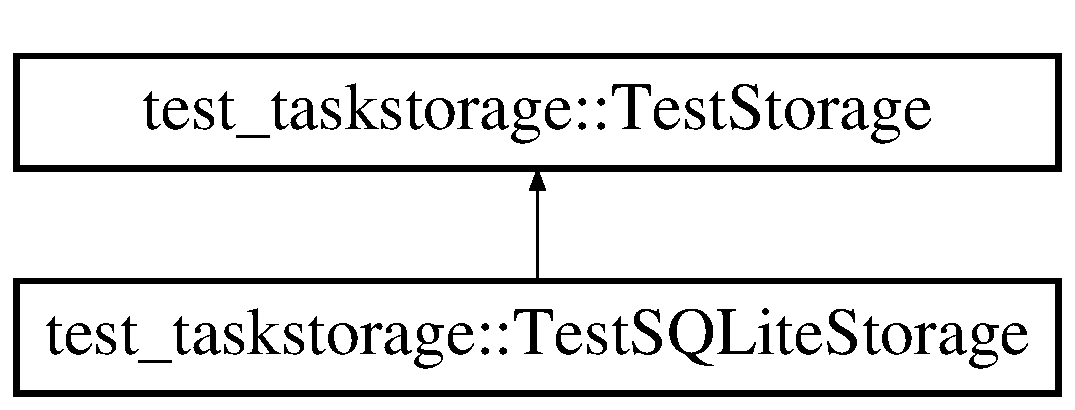
\includegraphics[height=2.000000cm]{classtest__taskstorage_1_1TestSQLiteStorage}
\end{center}
\end{figure}
\subsection*{\-Public \-Member \-Functions}
\begin{DoxyCompactItemize}
\item 
def \hyperlink{classtest__taskstorage_1_1TestSQLiteStorage_ae0d8cf19d4b45aa22960c66adf1d1101}{\-\_\-\-\_\-init\-\_\-\-\_\-}
\item 
def \hyperlink{classtest__taskstorage_1_1TestSQLiteStorage_a67becd24f719586fc3600410c58a5cf7}{set\-Up}
\item 
def \hyperlink{classtest__taskstorage_1_1TestSQLiteStorage_af7734cde6d1ef272761e8aee962fc32a}{tear\-Down}
\end{DoxyCompactItemize}
\subsection*{\-Public \-Attributes}
\begin{DoxyCompactItemize}
\item 
\hyperlink{classtest__taskstorage_1_1TestSQLiteStorage_af51f54f0c6c646bf1979afbc8005fa88}{my\-\_\-task}
\item 
\hyperlink{classtest__taskstorage_1_1TestSQLiteStorage_a0ebc44e061d815f63dcd5ef7edbc6cde}{test\-\_\-task\-\_\-dbname}
\item 
\hyperlink{classtest__taskstorage_1_1TestSQLiteStorage_ae03503042105ca995288e3128553870b}{task\-\_\-storage}
\end{DoxyCompactItemize}


\subsection{\-Detailed \-Description}
\-Tests specific to the \-S\-Q\-Lite\-Storage class. 

\-Tests that only apply to the implementation of the \-S\-Q\-Lite\-Storage class and not other task\-\_\-storage types. 

\-Definition at line 262 of file test\-\_\-taskstorage.\-py.



\subsection{\-Constructor \& \-Destructor \-Documentation}
\hypertarget{classtest__taskstorage_1_1TestSQLiteStorage_ae0d8cf19d4b45aa22960c66adf1d1101}{
\index{test\-\_\-taskstorage\-::\-Test\-S\-Q\-Lite\-Storage@{test\-\_\-taskstorage\-::\-Test\-S\-Q\-Lite\-Storage}!\-\_\-\-\_\-init\-\_\-\-\_\-@{\-\_\-\-\_\-init\-\_\-\-\_\-}}
\index{\-\_\-\-\_\-init\-\_\-\-\_\-@{\-\_\-\-\_\-init\-\_\-\-\_\-}!test_taskstorage::TestSQLiteStorage@{test\-\_\-taskstorage\-::\-Test\-S\-Q\-Lite\-Storage}}
\subsubsection[{\-\_\-\-\_\-init\-\_\-\-\_\-}]{\setlength{\rightskip}{0pt plus 5cm}def test\-\_\-taskstorage\-::\-Test\-S\-Q\-Lite\-Storage\-::\-\_\-\-\_\-init\-\_\-\-\_\- (
\begin{DoxyParamCaption}
\item[{}]{self, }
\item[{}]{method\-\_\-name}
\end{DoxyParamCaption}
)}}
\label{classtest__taskstorage_1_1TestSQLiteStorage_ae0d8cf19d4b45aa22960c66adf1d1101}


\-Reimplemented from \hyperlink{classtest__taskstorage_1_1TestStorage_a41a9bc77946b61981cdaebb9cdff74f8}{test\-\_\-taskstorage\-::\-Test\-Storage}.



\-Definition at line 264 of file test\-\_\-taskstorage.\-py.



\subsection{\-Member \-Function \-Documentation}
\hypertarget{classtest__taskstorage_1_1TestSQLiteStorage_a67becd24f719586fc3600410c58a5cf7}{
\index{test\-\_\-taskstorage\-::\-Test\-S\-Q\-Lite\-Storage@{test\-\_\-taskstorage\-::\-Test\-S\-Q\-Lite\-Storage}!set\-Up@{set\-Up}}
\index{set\-Up@{set\-Up}!test_taskstorage::TestSQLiteStorage@{test\-\_\-taskstorage\-::\-Test\-S\-Q\-Lite\-Storage}}
\subsubsection[{set\-Up}]{\setlength{\rightskip}{0pt plus 5cm}def test\-\_\-taskstorage\-::\-Test\-S\-Q\-Lite\-Storage\-::set\-Up (
\begin{DoxyParamCaption}
\item[{}]{self}
\end{DoxyParamCaption}
)}}
\label{classtest__taskstorage_1_1TestSQLiteStorage_a67becd24f719586fc3600410c58a5cf7}


\-Definition at line 267 of file test\-\_\-taskstorage.\-py.

\hypertarget{classtest__taskstorage_1_1TestSQLiteStorage_af7734cde6d1ef272761e8aee962fc32a}{
\index{test\-\_\-taskstorage\-::\-Test\-S\-Q\-Lite\-Storage@{test\-\_\-taskstorage\-::\-Test\-S\-Q\-Lite\-Storage}!tear\-Down@{tear\-Down}}
\index{tear\-Down@{tear\-Down}!test_taskstorage::TestSQLiteStorage@{test\-\_\-taskstorage\-::\-Test\-S\-Q\-Lite\-Storage}}
\subsubsection[{tear\-Down}]{\setlength{\rightskip}{0pt plus 5cm}def test\-\_\-taskstorage\-::\-Test\-S\-Q\-Lite\-Storage\-::tear\-Down (
\begin{DoxyParamCaption}
\item[{}]{self}
\end{DoxyParamCaption}
)}}
\label{classtest__taskstorage_1_1TestSQLiteStorage_af7734cde6d1ef272761e8aee962fc32a}


\-Definition at line 280 of file test\-\_\-taskstorage.\-py.



\subsection{\-Member \-Data \-Documentation}
\hypertarget{classtest__taskstorage_1_1TestSQLiteStorage_af51f54f0c6c646bf1979afbc8005fa88}{
\index{test\-\_\-taskstorage\-::\-Test\-S\-Q\-Lite\-Storage@{test\-\_\-taskstorage\-::\-Test\-S\-Q\-Lite\-Storage}!my\-\_\-task@{my\-\_\-task}}
\index{my\-\_\-task@{my\-\_\-task}!test_taskstorage::TestSQLiteStorage@{test\-\_\-taskstorage\-::\-Test\-S\-Q\-Lite\-Storage}}
\subsubsection[{my\-\_\-task}]{\setlength{\rightskip}{0pt plus 5cm}{\bf test\-\_\-taskstorage\-::\-Test\-S\-Q\-Lite\-Storage\-::my\-\_\-task}}}
\label{classtest__taskstorage_1_1TestSQLiteStorage_af51f54f0c6c646bf1979afbc8005fa88}


\-Reimplemented from \hyperlink{classtest__taskstorage_1_1TestStorage_a7d47cd41a51cd29b6f793d373599bd82}{test\-\_\-taskstorage\-::\-Test\-Storage}.



\-Definition at line 267 of file test\-\_\-taskstorage.\-py.

\hypertarget{classtest__taskstorage_1_1TestSQLiteStorage_ae03503042105ca995288e3128553870b}{
\index{test\-\_\-taskstorage\-::\-Test\-S\-Q\-Lite\-Storage@{test\-\_\-taskstorage\-::\-Test\-S\-Q\-Lite\-Storage}!task\-\_\-storage@{task\-\_\-storage}}
\index{task\-\_\-storage@{task\-\_\-storage}!test_taskstorage::TestSQLiteStorage@{test\-\_\-taskstorage\-::\-Test\-S\-Q\-Lite\-Storage}}
\subsubsection[{task\-\_\-storage}]{\setlength{\rightskip}{0pt plus 5cm}{\bf test\-\_\-taskstorage\-::\-Test\-S\-Q\-Lite\-Storage\-::task\-\_\-storage}}}
\label{classtest__taskstorage_1_1TestSQLiteStorage_ae03503042105ca995288e3128553870b}


\-Reimplemented from \hyperlink{classtest__taskstorage_1_1TestStorage_a414fec77c1f9ac66b58f26df514fc048}{test\-\_\-taskstorage\-::\-Test\-Storage}.



\-Definition at line 267 of file test\-\_\-taskstorage.\-py.

\hypertarget{classtest__taskstorage_1_1TestSQLiteStorage_a0ebc44e061d815f63dcd5ef7edbc6cde}{
\index{test\-\_\-taskstorage\-::\-Test\-S\-Q\-Lite\-Storage@{test\-\_\-taskstorage\-::\-Test\-S\-Q\-Lite\-Storage}!test\-\_\-task\-\_\-dbname@{test\-\_\-task\-\_\-dbname}}
\index{test\-\_\-task\-\_\-dbname@{test\-\_\-task\-\_\-dbname}!test_taskstorage::TestSQLiteStorage@{test\-\_\-taskstorage\-::\-Test\-S\-Q\-Lite\-Storage}}
\subsubsection[{test\-\_\-task\-\_\-dbname}]{\setlength{\rightskip}{0pt plus 5cm}{\bf test\-\_\-taskstorage\-::\-Test\-S\-Q\-Lite\-Storage\-::test\-\_\-task\-\_\-dbname}}}
\label{classtest__taskstorage_1_1TestSQLiteStorage_a0ebc44e061d815f63dcd5ef7edbc6cde}


\-Definition at line 267 of file test\-\_\-taskstorage.\-py.



\-The documentation for this class was generated from the following file\-:\begin{DoxyCompactItemize}
\item 
/home/scott/school/capstone/\-Task-\/\-Organizer/src/test/\hyperlink{test__taskstorage_8py}{test\-\_\-taskstorage.\-py}\end{DoxyCompactItemize}

\hypertarget{classtest__taskstorage_1_1TestStorage}{
\section{test\-\_\-taskstorage\-:\-:\-Test\-Storage \-Class \-Reference}
\label{classtest__taskstorage_1_1TestStorage}\index{test\-\_\-taskstorage\-::\-Test\-Storage@{test\-\_\-taskstorage\-::\-Test\-Storage}}
}


\-Abstract tests for the child classes of the \-Storage class.  


\-Inheritance diagram for test\-\_\-taskstorage\-:\-:\-Test\-Storage\-:\begin{figure}[H]
\begin{center}
\leavevmode
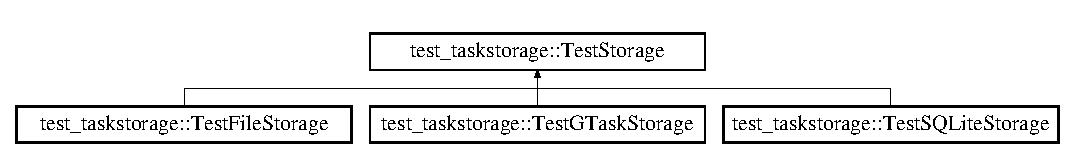
\includegraphics[height=1.689291cm]{classtest__taskstorage_1_1TestStorage}
\end{center}
\end{figure}
\subsection*{\-Public \-Member \-Functions}
\begin{DoxyCompactItemize}
\item 
def \hyperlink{classtest__taskstorage_1_1TestStorage_a41a9bc77946b61981cdaebb9cdff74f8}{\-\_\-\-\_\-init\-\_\-\-\_\-}
\item 
def \hyperlink{classtest__taskstorage_1_1TestStorage_aa6ca7dc5de002789d4d4ccdf67fdb08e}{test\-\_\-add}
\begin{DoxyCompactList}\small\item\em \-Tests that add() correctly adds a \-Task to storage. \end{DoxyCompactList}\item 
def \hyperlink{classtest__taskstorage_1_1TestStorage_a356b78c44916f1920e3a22c3dbca378f}{test\-\_\-find}
\begin{DoxyCompactList}\small\item\em \-Tests that find() correctly returns a \-Task given a key. \end{DoxyCompactList}\item 
def \hyperlink{classtest__taskstorage_1_1TestStorage_a09f937b953d03c22d7630817d90b9362}{test\-\_\-get\-\_\-all}
\begin{DoxyCompactList}\small\item\em \-Tests that get\-\_\-all() returns a list of all \-Tasks. \end{DoxyCompactList}\item 
def \hyperlink{classtest__taskstorage_1_1TestStorage_a9c88d63e97ce968fc34e873fa5d559c1}{test\-\_\-update}
\begin{DoxyCompactList}\small\item\em \-Tests that update() correctly updates a \-Task given a \-Task. \end{DoxyCompactList}\item 
def \hyperlink{classtest__taskstorage_1_1TestStorage_a437b4c393131de87ba9c555f92c5cb79}{test\-\_\-update\-\_\-no\-\_\-match}
\begin{DoxyCompactList}\small\item\em \-Tests updates()'s handling of no matching key. \end{DoxyCompactList}\item 
def \hyperlink{classtest__taskstorage_1_1TestStorage_a8b8bb9f5d0f2184902b2ce0dc1fd491d}{test\-\_\-delete}
\begin{DoxyCompactList}\small\item\em \-Tests that delete() correctly deletes a \-Task from storage. \end{DoxyCompactList}\item 
def \hyperlink{classtest__taskstorage_1_1TestStorage_a4eb39b2d44a6e283b5aa7fec7878a351}{test\-\_\-delete\-\_\-no\-\_\-match}
\begin{DoxyCompactList}\small\item\em \-Tests delete()'s handling of no matching key. \end{DoxyCompactList}\item 
def \hyperlink{classtest__taskstorage_1_1TestStorage_aef95d0237de543b3c466c0c0aa185b74}{test\-\_\-search}
\begin{DoxyCompactList}\small\item\em \-Tests that search() correctly returns a matching \-Task given a \-Task. \end{DoxyCompactList}\item 
def \hyperlink{classtest__taskstorage_1_1TestStorage_a5fa544513569dfa9632b5b34b2b30350}{test\-\_\-search\-\_\-not\-\_\-found}
\begin{DoxyCompactList}\small\item\em \-Tests search()'s behavior when no match is found. \end{DoxyCompactList}\end{DoxyCompactItemize}
\subsection*{\-Public \-Attributes}
\begin{DoxyCompactItemize}
\item 
\hyperlink{classtest__taskstorage_1_1TestStorage_a414fec77c1f9ac66b58f26df514fc048}{task\-\_\-storage}
\item 
\hyperlink{classtest__taskstorage_1_1TestStorage_a7d47cd41a51cd29b6f793d373599bd82}{my\-\_\-task}
\item 
\hyperlink{classtest__taskstorage_1_1TestStorage_ab9ddf07c905a5d38f3b48aa17411516e}{key}
\end{DoxyCompactItemize}


\subsection{\-Detailed \-Description}
\-Abstract tests for the child classes of the \-Storage class. 

\-This abstract test case's functions should be called only through a child test case. 

\-Definition at line 20 of file test\-\_\-taskstorage.\-py.



\subsection{\-Constructor \& \-Destructor \-Documentation}
\hypertarget{classtest__taskstorage_1_1TestStorage_a41a9bc77946b61981cdaebb9cdff74f8}{
\index{test\-\_\-taskstorage\-::\-Test\-Storage@{test\-\_\-taskstorage\-::\-Test\-Storage}!\-\_\-\-\_\-init\-\_\-\-\_\-@{\-\_\-\-\_\-init\-\_\-\-\_\-}}
\index{\-\_\-\-\_\-init\-\_\-\-\_\-@{\-\_\-\-\_\-init\-\_\-\-\_\-}!test_taskstorage::TestStorage@{test\-\_\-taskstorage\-::\-Test\-Storage}}
\subsubsection[{\-\_\-\-\_\-init\-\_\-\-\_\-}]{\setlength{\rightskip}{0pt plus 5cm}def test\-\_\-taskstorage\-::\-Test\-Storage\-::\-\_\-\-\_\-init\-\_\-\-\_\- (
\begin{DoxyParamCaption}
\item[{}]{self, }
\item[{}]{method\-\_\-name}
\end{DoxyParamCaption}
)}}
\label{classtest__taskstorage_1_1TestStorage_a41a9bc77946b61981cdaebb9cdff74f8}


\-Reimplemented in \hyperlink{classtest__taskstorage_1_1TestGTaskStorage_ae5d725daa8804f4bf01b56a5ba28303f}{test\-\_\-taskstorage\-::\-Test\-G\-Task\-Storage}, \hyperlink{classtest__taskstorage_1_1TestSQLiteStorage_ae0d8cf19d4b45aa22960c66adf1d1101}{test\-\_\-taskstorage\-::\-Test\-S\-Q\-Lite\-Storage}, and \hyperlink{classtest__taskstorage_1_1TestFileStorage_a3aeeb19983b93f40da74ca6f741bca7b}{test\-\_\-taskstorage\-::\-Test\-File\-Storage}.



\-Definition at line 22 of file test\-\_\-taskstorage.\-py.



\subsection{\-Member \-Function \-Documentation}
\hypertarget{classtest__taskstorage_1_1TestStorage_aa6ca7dc5de002789d4d4ccdf67fdb08e}{
\index{test\-\_\-taskstorage\-::\-Test\-Storage@{test\-\_\-taskstorage\-::\-Test\-Storage}!test\-\_\-add@{test\-\_\-add}}
\index{test\-\_\-add@{test\-\_\-add}!test_taskstorage::TestStorage@{test\-\_\-taskstorage\-::\-Test\-Storage}}
\subsubsection[{test\-\_\-add}]{\setlength{\rightskip}{0pt plus 5cm}def test\-\_\-taskstorage\-::\-Test\-Storage\-::test\-\_\-add (
\begin{DoxyParamCaption}
\item[{}]{self}
\end{DoxyParamCaption}
)}}
\label{classtest__taskstorage_1_1TestStorage_aa6ca7dc5de002789d4d4ccdf67fdb08e}


\-Tests that add() correctly adds a \-Task to storage. 



\-Definition at line 29 of file test\-\_\-taskstorage.\-py.

\hypertarget{classtest__taskstorage_1_1TestStorage_a8b8bb9f5d0f2184902b2ce0dc1fd491d}{
\index{test\-\_\-taskstorage\-::\-Test\-Storage@{test\-\_\-taskstorage\-::\-Test\-Storage}!test\-\_\-delete@{test\-\_\-delete}}
\index{test\-\_\-delete@{test\-\_\-delete}!test_taskstorage::TestStorage@{test\-\_\-taskstorage\-::\-Test\-Storage}}
\subsubsection[{test\-\_\-delete}]{\setlength{\rightskip}{0pt plus 5cm}def test\-\_\-taskstorage\-::\-Test\-Storage\-::test\-\_\-delete (
\begin{DoxyParamCaption}
\item[{}]{self}
\end{DoxyParamCaption}
)}}
\label{classtest__taskstorage_1_1TestStorage_a8b8bb9f5d0f2184902b2ce0dc1fd491d}


\-Tests that delete() correctly deletes a \-Task from storage. 



\-Definition at line 79 of file test\-\_\-taskstorage.\-py.

\hypertarget{classtest__taskstorage_1_1TestStorage_a4eb39b2d44a6e283b5aa7fec7878a351}{
\index{test\-\_\-taskstorage\-::\-Test\-Storage@{test\-\_\-taskstorage\-::\-Test\-Storage}!test\-\_\-delete\-\_\-no\-\_\-match@{test\-\_\-delete\-\_\-no\-\_\-match}}
\index{test\-\_\-delete\-\_\-no\-\_\-match@{test\-\_\-delete\-\_\-no\-\_\-match}!test_taskstorage::TestStorage@{test\-\_\-taskstorage\-::\-Test\-Storage}}
\subsubsection[{test\-\_\-delete\-\_\-no\-\_\-match}]{\setlength{\rightskip}{0pt plus 5cm}def test\-\_\-taskstorage\-::\-Test\-Storage\-::test\-\_\-delete\-\_\-no\-\_\-match (
\begin{DoxyParamCaption}
\item[{}]{self}
\end{DoxyParamCaption}
)}}
\label{classtest__taskstorage_1_1TestStorage_a4eb39b2d44a6e283b5aa7fec7878a351}


\-Tests delete()'s handling of no matching key. 



\-Definition at line 90 of file test\-\_\-taskstorage.\-py.

\hypertarget{classtest__taskstorage_1_1TestStorage_a356b78c44916f1920e3a22c3dbca378f}{
\index{test\-\_\-taskstorage\-::\-Test\-Storage@{test\-\_\-taskstorage\-::\-Test\-Storage}!test\-\_\-find@{test\-\_\-find}}
\index{test\-\_\-find@{test\-\_\-find}!test_taskstorage::TestStorage@{test\-\_\-taskstorage\-::\-Test\-Storage}}
\subsubsection[{test\-\_\-find}]{\setlength{\rightskip}{0pt plus 5cm}def test\-\_\-taskstorage\-::\-Test\-Storage\-::test\-\_\-find (
\begin{DoxyParamCaption}
\item[{}]{self}
\end{DoxyParamCaption}
)}}
\label{classtest__taskstorage_1_1TestStorage_a356b78c44916f1920e3a22c3dbca378f}


\-Tests that find() correctly returns a \-Task given a key. 



\-Definition at line 39 of file test\-\_\-taskstorage.\-py.

\hypertarget{classtest__taskstorage_1_1TestStorage_a09f937b953d03c22d7630817d90b9362}{
\index{test\-\_\-taskstorage\-::\-Test\-Storage@{test\-\_\-taskstorage\-::\-Test\-Storage}!test\-\_\-get\-\_\-all@{test\-\_\-get\-\_\-all}}
\index{test\-\_\-get\-\_\-all@{test\-\_\-get\-\_\-all}!test_taskstorage::TestStorage@{test\-\_\-taskstorage\-::\-Test\-Storage}}
\subsubsection[{test\-\_\-get\-\_\-all}]{\setlength{\rightskip}{0pt plus 5cm}def test\-\_\-taskstorage\-::\-Test\-Storage\-::test\-\_\-get\-\_\-all (
\begin{DoxyParamCaption}
\item[{}]{self}
\end{DoxyParamCaption}
)}}
\label{classtest__taskstorage_1_1TestStorage_a09f937b953d03c22d7630817d90b9362}


\-Tests that get\-\_\-all() returns a list of all \-Tasks. 



\-Definition at line 47 of file test\-\_\-taskstorage.\-py.

\hypertarget{classtest__taskstorage_1_1TestStorage_aef95d0237de543b3c466c0c0aa185b74}{
\index{test\-\_\-taskstorage\-::\-Test\-Storage@{test\-\_\-taskstorage\-::\-Test\-Storage}!test\-\_\-search@{test\-\_\-search}}
\index{test\-\_\-search@{test\-\_\-search}!test_taskstorage::TestStorage@{test\-\_\-taskstorage\-::\-Test\-Storage}}
\subsubsection[{test\-\_\-search}]{\setlength{\rightskip}{0pt plus 5cm}def test\-\_\-taskstorage\-::\-Test\-Storage\-::test\-\_\-search (
\begin{DoxyParamCaption}
\item[{}]{self}
\end{DoxyParamCaption}
)}}
\label{classtest__taskstorage_1_1TestStorage_aef95d0237de543b3c466c0c0aa185b74}


\-Tests that search() correctly returns a matching \-Task given a \-Task. 



\-Definition at line 101 of file test\-\_\-taskstorage.\-py.

\hypertarget{classtest__taskstorage_1_1TestStorage_a5fa544513569dfa9632b5b34b2b30350}{
\index{test\-\_\-taskstorage\-::\-Test\-Storage@{test\-\_\-taskstorage\-::\-Test\-Storage}!test\-\_\-search\-\_\-not\-\_\-found@{test\-\_\-search\-\_\-not\-\_\-found}}
\index{test\-\_\-search\-\_\-not\-\_\-found@{test\-\_\-search\-\_\-not\-\_\-found}!test_taskstorage::TestStorage@{test\-\_\-taskstorage\-::\-Test\-Storage}}
\subsubsection[{test\-\_\-search\-\_\-not\-\_\-found}]{\setlength{\rightskip}{0pt plus 5cm}def test\-\_\-taskstorage\-::\-Test\-Storage\-::test\-\_\-search\-\_\-not\-\_\-found (
\begin{DoxyParamCaption}
\item[{}]{self}
\end{DoxyParamCaption}
)}}
\label{classtest__taskstorage_1_1TestStorage_a5fa544513569dfa9632b5b34b2b30350}


\-Tests search()'s behavior when no match is found. 



\-Definition at line 110 of file test\-\_\-taskstorage.\-py.

\hypertarget{classtest__taskstorage_1_1TestStorage_a9c88d63e97ce968fc34e873fa5d559c1}{
\index{test\-\_\-taskstorage\-::\-Test\-Storage@{test\-\_\-taskstorage\-::\-Test\-Storage}!test\-\_\-update@{test\-\_\-update}}
\index{test\-\_\-update@{test\-\_\-update}!test_taskstorage::TestStorage@{test\-\_\-taskstorage\-::\-Test\-Storage}}
\subsubsection[{test\-\_\-update}]{\setlength{\rightskip}{0pt plus 5cm}def test\-\_\-taskstorage\-::\-Test\-Storage\-::test\-\_\-update (
\begin{DoxyParamCaption}
\item[{}]{self}
\end{DoxyParamCaption}
)}}
\label{classtest__taskstorage_1_1TestStorage_a9c88d63e97ce968fc34e873fa5d559c1}


\-Tests that update() correctly updates a \-Task given a \-Task. 



\-Definition at line 55 of file test\-\_\-taskstorage.\-py.

\hypertarget{classtest__taskstorage_1_1TestStorage_a437b4c393131de87ba9c555f92c5cb79}{
\index{test\-\_\-taskstorage\-::\-Test\-Storage@{test\-\_\-taskstorage\-::\-Test\-Storage}!test\-\_\-update\-\_\-no\-\_\-match@{test\-\_\-update\-\_\-no\-\_\-match}}
\index{test\-\_\-update\-\_\-no\-\_\-match@{test\-\_\-update\-\_\-no\-\_\-match}!test_taskstorage::TestStorage@{test\-\_\-taskstorage\-::\-Test\-Storage}}
\subsubsection[{test\-\_\-update\-\_\-no\-\_\-match}]{\setlength{\rightskip}{0pt plus 5cm}def test\-\_\-taskstorage\-::\-Test\-Storage\-::test\-\_\-update\-\_\-no\-\_\-match (
\begin{DoxyParamCaption}
\item[{}]{self}
\end{DoxyParamCaption}
)}}
\label{classtest__taskstorage_1_1TestStorage_a437b4c393131de87ba9c555f92c5cb79}


\-Tests updates()'s handling of no matching key. 



\-Definition at line 66 of file test\-\_\-taskstorage.\-py.



\subsection{\-Member \-Data \-Documentation}
\hypertarget{classtest__taskstorage_1_1TestStorage_ab9ddf07c905a5d38f3b48aa17411516e}{
\index{test\-\_\-taskstorage\-::\-Test\-Storage@{test\-\_\-taskstorage\-::\-Test\-Storage}!key@{key}}
\index{key@{key}!test_taskstorage::TestStorage@{test\-\_\-taskstorage\-::\-Test\-Storage}}
\subsubsection[{key}]{\setlength{\rightskip}{0pt plus 5cm}{\bf test\-\_\-taskstorage\-::\-Test\-Storage\-::key}}}
\label{classtest__taskstorage_1_1TestStorage_ab9ddf07c905a5d38f3b48aa17411516e}


\-Definition at line 66 of file test\-\_\-taskstorage.\-py.

\hypertarget{classtest__taskstorage_1_1TestStorage_a7d47cd41a51cd29b6f793d373599bd82}{
\index{test\-\_\-taskstorage\-::\-Test\-Storage@{test\-\_\-taskstorage\-::\-Test\-Storage}!my\-\_\-task@{my\-\_\-task}}
\index{my\-\_\-task@{my\-\_\-task}!test_taskstorage::TestStorage@{test\-\_\-taskstorage\-::\-Test\-Storage}}
\subsubsection[{my\-\_\-task}]{\setlength{\rightskip}{0pt plus 5cm}{\bf test\-\_\-taskstorage\-::\-Test\-Storage\-::my\-\_\-task}}}
\label{classtest__taskstorage_1_1TestStorage_a7d47cd41a51cd29b6f793d373599bd82}


\-Reimplemented in \hyperlink{classtest__taskstorage_1_1TestGTaskStorage_a64044ab25309aa17502a40daa5983923}{test\-\_\-taskstorage\-::\-Test\-G\-Task\-Storage}, \hyperlink{classtest__taskstorage_1_1TestSQLiteStorage_af51f54f0c6c646bf1979afbc8005fa88}{test\-\_\-taskstorage\-::\-Test\-S\-Q\-Lite\-Storage}, and \hyperlink{classtest__taskstorage_1_1TestFileStorage_a986e73f6663aa98ee3f90e1be3fa2515}{test\-\_\-taskstorage\-::\-Test\-File\-Storage}.



\-Definition at line 22 of file test\-\_\-taskstorage.\-py.

\hypertarget{classtest__taskstorage_1_1TestStorage_a414fec77c1f9ac66b58f26df514fc048}{
\index{test\-\_\-taskstorage\-::\-Test\-Storage@{test\-\_\-taskstorage\-::\-Test\-Storage}!task\-\_\-storage@{task\-\_\-storage}}
\index{task\-\_\-storage@{task\-\_\-storage}!test_taskstorage::TestStorage@{test\-\_\-taskstorage\-::\-Test\-Storage}}
\subsubsection[{task\-\_\-storage}]{\setlength{\rightskip}{0pt plus 5cm}{\bf test\-\_\-taskstorage\-::\-Test\-Storage\-::task\-\_\-storage}}}
\label{classtest__taskstorage_1_1TestStorage_a414fec77c1f9ac66b58f26df514fc048}


\-Reimplemented in \hyperlink{classtest__taskstorage_1_1TestGTaskStorage_abb748de83f5fdbc145f7570464fe13b7}{test\-\_\-taskstorage\-::\-Test\-G\-Task\-Storage}, \hyperlink{classtest__taskstorage_1_1TestSQLiteStorage_ae03503042105ca995288e3128553870b}{test\-\_\-taskstorage\-::\-Test\-S\-Q\-Lite\-Storage}, and \hyperlink{classtest__taskstorage_1_1TestFileStorage_af65fc75e8b921b475ea610cf3681e270}{test\-\_\-taskstorage\-::\-Test\-File\-Storage}.



\-Definition at line 22 of file test\-\_\-taskstorage.\-py.



\-The documentation for this class was generated from the following file\-:\begin{DoxyCompactItemize}
\item 
/home/scott/school/capstone/\-Task-\/\-Organizer/src/test/\hyperlink{test__taskstorage_8py}{test\-\_\-taskstorage.\-py}\end{DoxyCompactItemize}

\hypertarget{classtest__task_1_1TestTask}{
\section{test\-\_\-task\-:\-:\-Test\-Task \-Class \-Reference}
\label{classtest__task_1_1TestTask}\index{test\-\_\-task\-::\-Test\-Task@{test\-\_\-task\-::\-Test\-Task}}
}


\-Tests \-Task objects.  


\subsection*{\-Public \-Member \-Functions}
\begin{DoxyCompactItemize}
\item 
def \hyperlink{classtest__task_1_1TestTask_aa16cc539a6857b7be141a5b45d55b443}{set\-Up}
\item 
def \hyperlink{classtest__task_1_1TestTask_a31e0d5deaf86abc966ec43c06003b994}{tear\-Down}
\item 
def \hyperlink{classtest__task_1_1TestTask_a8168a86d54e2cc00240e812271a2d5b3}{test\-\_\-equal}
\begin{DoxyCompactList}\small\item\em \-Tests a \-Task's handling when compared to an equivalent \-Task. \end{DoxyCompactList}\item 
def \hyperlink{classtest__task_1_1TestTask_a2e3b19feba163771555b4625358ef890}{test\-\_\-equal\-\_\-false}
\begin{DoxyCompactList}\small\item\em \-Tests a \-Task's handling when == returns \-False. \end{DoxyCompactList}\item 
def \hyperlink{classtest__task_1_1TestTask_a29b698f43d3f816aec619e3d3de71673}{test\-\_\-not\-\_\-equal}
\begin{DoxyCompactList}\small\item\em \-Tests a \-Task's handling when != returns \-True. \end{DoxyCompactList}\item 
def \hyperlink{classtest__task_1_1TestTask_a8419f9c14d8e9475b6dfa7bc75fbe285}{test\-\_\-equal\-\_\-false\-\_\-instance}
\begin{DoxyCompactList}\small\item\em \-Tests a \-Task's handling when == compares to a \-Task instance. \end{DoxyCompactList}\item 
def \hyperlink{classtest__task_1_1TestTask_a34481ea4940b6104d28d8bb2faaed462}{test\-\_\-not\-\_\-equal\-\_\-instance}
\begin{DoxyCompactList}\small\item\em \-Tests a \-Task's handling when != compares to a non-\/\-Task instance. \end{DoxyCompactList}\end{DoxyCompactItemize}
\subsection*{\-Public \-Attributes}
\begin{DoxyCompactItemize}
\item 
\hyperlink{classtest__task_1_1TestTask_ac2f3d00c02fd9907ce4427cc1b0c968f}{my\-\_\-task}
\end{DoxyCompactItemize}


\subsection{\-Detailed \-Description}
\-Tests \-Task objects. 

\-Definition at line 8 of file test\-\_\-task.\-py.



\subsection{\-Member \-Function \-Documentation}
\hypertarget{classtest__task_1_1TestTask_aa16cc539a6857b7be141a5b45d55b443}{
\index{test\-\_\-task\-::\-Test\-Task@{test\-\_\-task\-::\-Test\-Task}!set\-Up@{set\-Up}}
\index{set\-Up@{set\-Up}!test_task::TestTask@{test\-\_\-task\-::\-Test\-Task}}
\subsubsection[{set\-Up}]{\setlength{\rightskip}{0pt plus 5cm}def test\-\_\-task\-::\-Test\-Task\-::set\-Up (
\begin{DoxyParamCaption}
\item[{}]{self}
\end{DoxyParamCaption}
)}}
\label{classtest__task_1_1TestTask_aa16cc539a6857b7be141a5b45d55b443}


\-Definition at line 10 of file test\-\_\-task.\-py.

\hypertarget{classtest__task_1_1TestTask_a31e0d5deaf86abc966ec43c06003b994}{
\index{test\-\_\-task\-::\-Test\-Task@{test\-\_\-task\-::\-Test\-Task}!tear\-Down@{tear\-Down}}
\index{tear\-Down@{tear\-Down}!test_task::TestTask@{test\-\_\-task\-::\-Test\-Task}}
\subsubsection[{tear\-Down}]{\setlength{\rightskip}{0pt plus 5cm}def test\-\_\-task\-::\-Test\-Task\-::tear\-Down (
\begin{DoxyParamCaption}
\item[{}]{self}
\end{DoxyParamCaption}
)}}
\label{classtest__task_1_1TestTask_a31e0d5deaf86abc966ec43c06003b994}


\-Definition at line 16 of file test\-\_\-task.\-py.

\hypertarget{classtest__task_1_1TestTask_a8168a86d54e2cc00240e812271a2d5b3}{
\index{test\-\_\-task\-::\-Test\-Task@{test\-\_\-task\-::\-Test\-Task}!test\-\_\-equal@{test\-\_\-equal}}
\index{test\-\_\-equal@{test\-\_\-equal}!test_task::TestTask@{test\-\_\-task\-::\-Test\-Task}}
\subsubsection[{test\-\_\-equal}]{\setlength{\rightskip}{0pt plus 5cm}def test\-\_\-task\-::\-Test\-Task\-::test\-\_\-equal (
\begin{DoxyParamCaption}
\item[{}]{self}
\end{DoxyParamCaption}
)}}
\label{classtest__task_1_1TestTask_a8168a86d54e2cc00240e812271a2d5b3}


\-Tests a \-Task's handling when compared to an equivalent \-Task. 



\-Definition at line 22 of file test\-\_\-task.\-py.

\hypertarget{classtest__task_1_1TestTask_a2e3b19feba163771555b4625358ef890}{
\index{test\-\_\-task\-::\-Test\-Task@{test\-\_\-task\-::\-Test\-Task}!test\-\_\-equal\-\_\-false@{test\-\_\-equal\-\_\-false}}
\index{test\-\_\-equal\-\_\-false@{test\-\_\-equal\-\_\-false}!test_task::TestTask@{test\-\_\-task\-::\-Test\-Task}}
\subsubsection[{test\-\_\-equal\-\_\-false}]{\setlength{\rightskip}{0pt plus 5cm}def test\-\_\-task\-::\-Test\-Task\-::test\-\_\-equal\-\_\-false (
\begin{DoxyParamCaption}
\item[{}]{self}
\end{DoxyParamCaption}
)}}
\label{classtest__task_1_1TestTask_a2e3b19feba163771555b4625358ef890}


\-Tests a \-Task's handling when == returns \-False. 



\-Definition at line 29 of file test\-\_\-task.\-py.

\hypertarget{classtest__task_1_1TestTask_a8419f9c14d8e9475b6dfa7bc75fbe285}{
\index{test\-\_\-task\-::\-Test\-Task@{test\-\_\-task\-::\-Test\-Task}!test\-\_\-equal\-\_\-false\-\_\-instance@{test\-\_\-equal\-\_\-false\-\_\-instance}}
\index{test\-\_\-equal\-\_\-false\-\_\-instance@{test\-\_\-equal\-\_\-false\-\_\-instance}!test_task::TestTask@{test\-\_\-task\-::\-Test\-Task}}
\subsubsection[{test\-\_\-equal\-\_\-false\-\_\-instance}]{\setlength{\rightskip}{0pt plus 5cm}def test\-\_\-task\-::\-Test\-Task\-::test\-\_\-equal\-\_\-false\-\_\-instance (
\begin{DoxyParamCaption}
\item[{}]{self}
\end{DoxyParamCaption}
)}}
\label{classtest__task_1_1TestTask_a8419f9c14d8e9475b6dfa7bc75fbe285}


\-Tests a \-Task's handling when == compares to a \-Task instance. 



\-Definition at line 50 of file test\-\_\-task.\-py.

\hypertarget{classtest__task_1_1TestTask_a29b698f43d3f816aec619e3d3de71673}{
\index{test\-\_\-task\-::\-Test\-Task@{test\-\_\-task\-::\-Test\-Task}!test\-\_\-not\-\_\-equal@{test\-\_\-not\-\_\-equal}}
\index{test\-\_\-not\-\_\-equal@{test\-\_\-not\-\_\-equal}!test_task::TestTask@{test\-\_\-task\-::\-Test\-Task}}
\subsubsection[{test\-\_\-not\-\_\-equal}]{\setlength{\rightskip}{0pt plus 5cm}def test\-\_\-task\-::\-Test\-Task\-::test\-\_\-not\-\_\-equal (
\begin{DoxyParamCaption}
\item[{}]{self}
\end{DoxyParamCaption}
)}}
\label{classtest__task_1_1TestTask_a29b698f43d3f816aec619e3d3de71673}


\-Tests a \-Task's handling when != returns \-True. 



\-Definition at line 38 of file test\-\_\-task.\-py.

\hypertarget{classtest__task_1_1TestTask_a34481ea4940b6104d28d8bb2faaed462}{
\index{test\-\_\-task\-::\-Test\-Task@{test\-\_\-task\-::\-Test\-Task}!test\-\_\-not\-\_\-equal\-\_\-instance@{test\-\_\-not\-\_\-equal\-\_\-instance}}
\index{test\-\_\-not\-\_\-equal\-\_\-instance@{test\-\_\-not\-\_\-equal\-\_\-instance}!test_task::TestTask@{test\-\_\-task\-::\-Test\-Task}}
\subsubsection[{test\-\_\-not\-\_\-equal\-\_\-instance}]{\setlength{\rightskip}{0pt plus 5cm}def test\-\_\-task\-::\-Test\-Task\-::test\-\_\-not\-\_\-equal\-\_\-instance (
\begin{DoxyParamCaption}
\item[{}]{self}
\end{DoxyParamCaption}
)}}
\label{classtest__task_1_1TestTask_a34481ea4940b6104d28d8bb2faaed462}


\-Tests a \-Task's handling when != compares to a non-\/\-Task instance. 



\-Definition at line 59 of file test\-\_\-task.\-py.



\subsection{\-Member \-Data \-Documentation}
\hypertarget{classtest__task_1_1TestTask_ac2f3d00c02fd9907ce4427cc1b0c968f}{
\index{test\-\_\-task\-::\-Test\-Task@{test\-\_\-task\-::\-Test\-Task}!my\-\_\-task@{my\-\_\-task}}
\index{my\-\_\-task@{my\-\_\-task}!test_task::TestTask@{test\-\_\-task\-::\-Test\-Task}}
\subsubsection[{my\-\_\-task}]{\setlength{\rightskip}{0pt plus 5cm}{\bf test\-\_\-task\-::\-Test\-Task\-::my\-\_\-task}}}
\label{classtest__task_1_1TestTask_ac2f3d00c02fd9907ce4427cc1b0c968f}


\-Definition at line 10 of file test\-\_\-task.\-py.



\-The documentation for this class was generated from the following file\-:\begin{DoxyCompactItemize}
\item 
/home/scott/school/capstone/\-Task-\/\-Organizer/src/test/\hyperlink{test__task_8py}{test\-\_\-task.\-py}\end{DoxyCompactItemize}

\hypertarget{classtest__taskcontroller_1_1TestTaskController}{
\section{test\-\_\-taskcontroller\-:\-:\-Test\-Task\-Controller \-Class \-Reference}
\label{classtest__taskcontroller_1_1TestTaskController}\index{test\-\_\-taskcontroller\-::\-Test\-Task\-Controller@{test\-\_\-taskcontroller\-::\-Test\-Task\-Controller}}
}


\-Abstract tests for child tests using specific storage types.  


\-Inheritance diagram for test\-\_\-taskcontroller\-:\-:\-Test\-Task\-Controller\-:\begin{figure}[H]
\begin{center}
\leavevmode
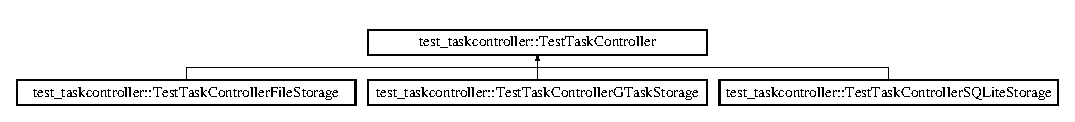
\includegraphics[height=1.185185cm]{classtest__taskcontroller_1_1TestTaskController}
\end{center}
\end{figure}
\subsection*{\-Public \-Member \-Functions}
\begin{DoxyCompactItemize}
\item 
def \hyperlink{classtest__taskcontroller_1_1TestTaskController_a2ec547bb413edbb40c0ae582dd2466bd}{\-\_\-\-\_\-init\-\_\-\-\_\-}
\item 
def \hyperlink{classtest__taskcontroller_1_1TestTaskController_a89989d1173db14268c0329ad98d304d5}{add\-\_\-task}
\begin{DoxyCompactList}\small\item\em \-Helper function to add \-Task to storage as given dict. \end{DoxyCompactList}\item 
def \hyperlink{classtest__taskcontroller_1_1TestTaskController_a37d53351ab2b48968965ef22ad6c4a18}{find\-\_\-task}
\begin{DoxyCompactList}\small\item\em \-Helper function to find \-Task in storage when given key. \end{DoxyCompactList}\item 
def \hyperlink{classtest__taskcontroller_1_1TestTaskController_a9f241994236f76865549287f630b43ef}{test\-\_\-add}
\begin{DoxyCompactList}\small\item\em \-Tests that add() correctly adds the arg dict as a \-Task to storage. \end{DoxyCompactList}\item 
def \hyperlink{classtest__taskcontroller_1_1TestTaskController_a8921a89235720f678cef5ee895e34cee}{test\-\_\-find}
\begin{DoxyCompactList}\small\item\em \-Tests that find() correctly returns a \-Task given an arg dict. \end{DoxyCompactList}\item 
def \hyperlink{classtest__taskcontroller_1_1TestTaskController_ac5577377f866469b155257d7c2674b8c}{test\-\_\-find\-\_\-all}
\begin{DoxyCompactList}\small\item\em \-Tests that find() correctly returns all \-Tasks when given no key. \end{DoxyCompactList}\item 
def \hyperlink{classtest__taskcontroller_1_1TestTaskController_afc1f00967a02557cf405a3428d6d86b2}{test\-\_\-edit}
\begin{DoxyCompactList}\small\item\em \-Tests that edit() correctly modifies a \-Task given an arg dict. \end{DoxyCompactList}\item 
def \hyperlink{classtest__taskcontroller_1_1TestTaskController_ac5d4cb8d40e6976c97f7bd9f0d0e5dc4}{test\-\_\-edit\-\_\-none}
\begin{DoxyCompactList}\small\item\em \-Tests edit()'s handling of arg dicts with empty attributes. \end{DoxyCompactList}\item 
def \hyperlink{classtest__taskcontroller_1_1TestTaskController_a2bf53edfdfd95abe028ce4ada0644263}{test\-\_\-delete}
\begin{DoxyCompactList}\small\item\em \-Tests that delete() correctly deletes a \-Task given an arg dict. \end{DoxyCompactList}\end{DoxyCompactItemize}
\subsection*{\-Public \-Attributes}
\begin{DoxyCompactItemize}
\item 
\hyperlink{classtest__taskcontroller_1_1TestTaskController_a16cbd17e4ad8bf93e164813b77313942}{interface\-\_\-controller}
\item 
\hyperlink{classtest__taskcontroller_1_1TestTaskController_a450431cde03f14169cd5ac04db704ab6}{title}
\item 
\hyperlink{classtest__taskcontroller_1_1TestTaskController_a9825f47dfebf3e25f03548d51d1d07d1}{notes}
\item 
\hyperlink{classtest__taskcontroller_1_1TestTaskController_a8b748405763b73406ca9cfafe467c0a1}{added\-\_\-task}
\end{DoxyCompactItemize}


\subsection{\-Detailed \-Description}
\-Abstract tests for child tests using specific storage types. 

\-Generic tests used by all \-Task\-Controller tests undependent on what storage type they are using. \-These tests should never be called directly. 

\-Definition at line 15 of file test\-\_\-taskcontroller.\-py.



\subsection{\-Constructor \& \-Destructor \-Documentation}
\hypertarget{classtest__taskcontroller_1_1TestTaskController_a2ec547bb413edbb40c0ae582dd2466bd}{
\index{test\-\_\-taskcontroller\-::\-Test\-Task\-Controller@{test\-\_\-taskcontroller\-::\-Test\-Task\-Controller}!\-\_\-\-\_\-init\-\_\-\-\_\-@{\-\_\-\-\_\-init\-\_\-\-\_\-}}
\index{\-\_\-\-\_\-init\-\_\-\-\_\-@{\-\_\-\-\_\-init\-\_\-\-\_\-}!test_taskcontroller::TestTaskController@{test\-\_\-taskcontroller\-::\-Test\-Task\-Controller}}
\subsubsection[{\-\_\-\-\_\-init\-\_\-\-\_\-}]{\setlength{\rightskip}{0pt plus 5cm}def test\-\_\-taskcontroller\-::\-Test\-Task\-Controller\-::\-\_\-\-\_\-init\-\_\-\-\_\- (
\begin{DoxyParamCaption}
\item[{}]{self, }
\item[{}]{method\-\_\-name}
\end{DoxyParamCaption}
)}}
\label{classtest__taskcontroller_1_1TestTaskController_a2ec547bb413edbb40c0ae582dd2466bd}


\-Reimplemented in \hyperlink{classtest__taskcontroller_1_1TestTaskControllerGTaskStorage_a6486ee999987082360633f99b887af86}{test\-\_\-taskcontroller\-::\-Test\-Task\-Controller\-G\-Task\-Storage}, \hyperlink{classtest__taskcontroller_1_1TestTaskControllerSQLiteStorage_a29417d2c4aee8c9bd135faff67203edc}{test\-\_\-taskcontroller\-::\-Test\-Task\-Controller\-S\-Q\-Lite\-Storage}, and \hyperlink{classtest__taskcontroller_1_1TestTaskControllerFileStorage_a1f63de1b9c566d073b4a11c5a49530c6}{test\-\_\-taskcontroller\-::\-Test\-Task\-Controller\-File\-Storage}.



\-Definition at line 17 of file test\-\_\-taskcontroller.\-py.



\subsection{\-Member \-Function \-Documentation}
\hypertarget{classtest__taskcontroller_1_1TestTaskController_a89989d1173db14268c0329ad98d304d5}{
\index{test\-\_\-taskcontroller\-::\-Test\-Task\-Controller@{test\-\_\-taskcontroller\-::\-Test\-Task\-Controller}!add\-\_\-task@{add\-\_\-task}}
\index{add\-\_\-task@{add\-\_\-task}!test_taskcontroller::TestTaskController@{test\-\_\-taskcontroller\-::\-Test\-Task\-Controller}}
\subsubsection[{add\-\_\-task}]{\setlength{\rightskip}{0pt plus 5cm}def test\-\_\-taskcontroller\-::\-Test\-Task\-Controller\-::add\-\_\-task (
\begin{DoxyParamCaption}
\item[{}]{self}
\end{DoxyParamCaption}
)}}
\label{classtest__taskcontroller_1_1TestTaskController_a89989d1173db14268c0329ad98d304d5}


\-Helper function to add \-Task to storage as given dict. 



\-Definition at line 26 of file test\-\_\-taskcontroller.\-py.

\hypertarget{classtest__taskcontroller_1_1TestTaskController_a37d53351ab2b48968965ef22ad6c4a18}{
\index{test\-\_\-taskcontroller\-::\-Test\-Task\-Controller@{test\-\_\-taskcontroller\-::\-Test\-Task\-Controller}!find\-\_\-task@{find\-\_\-task}}
\index{find\-\_\-task@{find\-\_\-task}!test_taskcontroller::TestTaskController@{test\-\_\-taskcontroller\-::\-Test\-Task\-Controller}}
\subsubsection[{find\-\_\-task}]{\setlength{\rightskip}{0pt plus 5cm}def test\-\_\-taskcontroller\-::\-Test\-Task\-Controller\-::find\-\_\-task (
\begin{DoxyParamCaption}
\item[{}]{self, }
\item[{}]{task\-\_\-key}
\end{DoxyParamCaption}
)}}
\label{classtest__taskcontroller_1_1TestTaskController_a37d53351ab2b48968965ef22ad6c4a18}


\-Helper function to find \-Task in storage when given key. 



\-Definition at line 38 of file test\-\_\-taskcontroller.\-py.

\hypertarget{classtest__taskcontroller_1_1TestTaskController_a9f241994236f76865549287f630b43ef}{
\index{test\-\_\-taskcontroller\-::\-Test\-Task\-Controller@{test\-\_\-taskcontroller\-::\-Test\-Task\-Controller}!test\-\_\-add@{test\-\_\-add}}
\index{test\-\_\-add@{test\-\_\-add}!test_taskcontroller::TestTaskController@{test\-\_\-taskcontroller\-::\-Test\-Task\-Controller}}
\subsubsection[{test\-\_\-add}]{\setlength{\rightskip}{0pt plus 5cm}def test\-\_\-taskcontroller\-::\-Test\-Task\-Controller\-::test\-\_\-add (
\begin{DoxyParamCaption}
\item[{}]{self}
\end{DoxyParamCaption}
)}}
\label{classtest__taskcontroller_1_1TestTaskController_a9f241994236f76865549287f630b43ef}


\-Tests that add() correctly adds the arg dict as a \-Task to storage. 



\-Definition at line 50 of file test\-\_\-taskcontroller.\-py.

\hypertarget{classtest__taskcontroller_1_1TestTaskController_a2bf53edfdfd95abe028ce4ada0644263}{
\index{test\-\_\-taskcontroller\-::\-Test\-Task\-Controller@{test\-\_\-taskcontroller\-::\-Test\-Task\-Controller}!test\-\_\-delete@{test\-\_\-delete}}
\index{test\-\_\-delete@{test\-\_\-delete}!test_taskcontroller::TestTaskController@{test\-\_\-taskcontroller\-::\-Test\-Task\-Controller}}
\subsubsection[{test\-\_\-delete}]{\setlength{\rightskip}{0pt plus 5cm}def test\-\_\-taskcontroller\-::\-Test\-Task\-Controller\-::test\-\_\-delete (
\begin{DoxyParamCaption}
\item[{}]{self}
\end{DoxyParamCaption}
)}}
\label{classtest__taskcontroller_1_1TestTaskController_a2bf53edfdfd95abe028ce4ada0644263}


\-Tests that delete() correctly deletes a \-Task given an arg dict. 



\-Definition at line 117 of file test\-\_\-taskcontroller.\-py.

\hypertarget{classtest__taskcontroller_1_1TestTaskController_afc1f00967a02557cf405a3428d6d86b2}{
\index{test\-\_\-taskcontroller\-::\-Test\-Task\-Controller@{test\-\_\-taskcontroller\-::\-Test\-Task\-Controller}!test\-\_\-edit@{test\-\_\-edit}}
\index{test\-\_\-edit@{test\-\_\-edit}!test_taskcontroller::TestTaskController@{test\-\_\-taskcontroller\-::\-Test\-Task\-Controller}}
\subsubsection[{test\-\_\-edit}]{\setlength{\rightskip}{0pt plus 5cm}def test\-\_\-taskcontroller\-::\-Test\-Task\-Controller\-::test\-\_\-edit (
\begin{DoxyParamCaption}
\item[{}]{self}
\end{DoxyParamCaption}
)}}
\label{classtest__taskcontroller_1_1TestTaskController_afc1f00967a02557cf405a3428d6d86b2}


\-Tests that edit() correctly modifies a \-Task given an arg dict. 



\-Definition at line 82 of file test\-\_\-taskcontroller.\-py.

\hypertarget{classtest__taskcontroller_1_1TestTaskController_ac5d4cb8d40e6976c97f7bd9f0d0e5dc4}{
\index{test\-\_\-taskcontroller\-::\-Test\-Task\-Controller@{test\-\_\-taskcontroller\-::\-Test\-Task\-Controller}!test\-\_\-edit\-\_\-none@{test\-\_\-edit\-\_\-none}}
\index{test\-\_\-edit\-\_\-none@{test\-\_\-edit\-\_\-none}!test_taskcontroller::TestTaskController@{test\-\_\-taskcontroller\-::\-Test\-Task\-Controller}}
\subsubsection[{test\-\_\-edit\-\_\-none}]{\setlength{\rightskip}{0pt plus 5cm}def test\-\_\-taskcontroller\-::\-Test\-Task\-Controller\-::test\-\_\-edit\-\_\-none (
\begin{DoxyParamCaption}
\item[{}]{self}
\end{DoxyParamCaption}
)}}
\label{classtest__taskcontroller_1_1TestTaskController_ac5d4cb8d40e6976c97f7bd9f0d0e5dc4}


\-Tests edit()'s handling of arg dicts with empty attributes. 



\-Definition at line 99 of file test\-\_\-taskcontroller.\-py.

\hypertarget{classtest__taskcontroller_1_1TestTaskController_a8921a89235720f678cef5ee895e34cee}{
\index{test\-\_\-taskcontroller\-::\-Test\-Task\-Controller@{test\-\_\-taskcontroller\-::\-Test\-Task\-Controller}!test\-\_\-find@{test\-\_\-find}}
\index{test\-\_\-find@{test\-\_\-find}!test_taskcontroller::TestTaskController@{test\-\_\-taskcontroller\-::\-Test\-Task\-Controller}}
\subsubsection[{test\-\_\-find}]{\setlength{\rightskip}{0pt plus 5cm}def test\-\_\-taskcontroller\-::\-Test\-Task\-Controller\-::test\-\_\-find (
\begin{DoxyParamCaption}
\item[{}]{self}
\end{DoxyParamCaption}
)}}
\label{classtest__taskcontroller_1_1TestTaskController_a8921a89235720f678cef5ee895e34cee}


\-Tests that find() correctly returns a \-Task given an arg dict. 



\-Definition at line 57 of file test\-\_\-taskcontroller.\-py.

\hypertarget{classtest__taskcontroller_1_1TestTaskController_ac5577377f866469b155257d7c2674b8c}{
\index{test\-\_\-taskcontroller\-::\-Test\-Task\-Controller@{test\-\_\-taskcontroller\-::\-Test\-Task\-Controller}!test\-\_\-find\-\_\-all@{test\-\_\-find\-\_\-all}}
\index{test\-\_\-find\-\_\-all@{test\-\_\-find\-\_\-all}!test_taskcontroller::TestTaskController@{test\-\_\-taskcontroller\-::\-Test\-Task\-Controller}}
\subsubsection[{test\-\_\-find\-\_\-all}]{\setlength{\rightskip}{0pt plus 5cm}def test\-\_\-taskcontroller\-::\-Test\-Task\-Controller\-::test\-\_\-find\-\_\-all (
\begin{DoxyParamCaption}
\item[{}]{self}
\end{DoxyParamCaption}
)}}
\label{classtest__taskcontroller_1_1TestTaskController_ac5577377f866469b155257d7c2674b8c}


\-Tests that find() correctly returns all \-Tasks when given no key. 



\-Definition at line 66 of file test\-\_\-taskcontroller.\-py.



\subsection{\-Member \-Data \-Documentation}
\hypertarget{classtest__taskcontroller_1_1TestTaskController_a8b748405763b73406ca9cfafe467c0a1}{
\index{test\-\_\-taskcontroller\-::\-Test\-Task\-Controller@{test\-\_\-taskcontroller\-::\-Test\-Task\-Controller}!added\-\_\-task@{added\-\_\-task}}
\index{added\-\_\-task@{added\-\_\-task}!test_taskcontroller::TestTaskController@{test\-\_\-taskcontroller\-::\-Test\-Task\-Controller}}
\subsubsection[{added\-\_\-task}]{\setlength{\rightskip}{0pt plus 5cm}{\bf test\-\_\-taskcontroller\-::\-Test\-Task\-Controller\-::added\-\_\-task}}}
\label{classtest__taskcontroller_1_1TestTaskController_a8b748405763b73406ca9cfafe467c0a1}


\-Reimplemented in \hyperlink{classtest__taskcontroller_1_1TestTaskControllerGTaskStorage_a150fa26a41cdce7d5d753edf43d5a09e}{test\-\_\-taskcontroller\-::\-Test\-Task\-Controller\-G\-Task\-Storage}, \hyperlink{classtest__taskcontroller_1_1TestTaskControllerSQLiteStorage_aa69b7c38504f5c50040bec6b0fcc73c3}{test\-\_\-taskcontroller\-::\-Test\-Task\-Controller\-S\-Q\-Lite\-Storage}, and \hyperlink{classtest__taskcontroller_1_1TestTaskControllerFileStorage_a5b9b16c50e8e488cbc066f5db85bca64}{test\-\_\-taskcontroller\-::\-Test\-Task\-Controller\-File\-Storage}.



\-Definition at line 17 of file test\-\_\-taskcontroller.\-py.

\hypertarget{classtest__taskcontroller_1_1TestTaskController_a16cbd17e4ad8bf93e164813b77313942}{
\index{test\-\_\-taskcontroller\-::\-Test\-Task\-Controller@{test\-\_\-taskcontroller\-::\-Test\-Task\-Controller}!interface\-\_\-controller@{interface\-\_\-controller}}
\index{interface\-\_\-controller@{interface\-\_\-controller}!test_taskcontroller::TestTaskController@{test\-\_\-taskcontroller\-::\-Test\-Task\-Controller}}
\subsubsection[{interface\-\_\-controller}]{\setlength{\rightskip}{0pt plus 5cm}{\bf test\-\_\-taskcontroller\-::\-Test\-Task\-Controller\-::interface\-\_\-controller}}}
\label{classtest__taskcontroller_1_1TestTaskController_a16cbd17e4ad8bf93e164813b77313942}


\-Reimplemented in \hyperlink{classtest__taskcontroller_1_1TestTaskControllerGTaskStorage_ac6b50d155cf6a1b6e013aec3b5239506}{test\-\_\-taskcontroller\-::\-Test\-Task\-Controller\-G\-Task\-Storage}, \hyperlink{classtest__taskcontroller_1_1TestTaskControllerSQLiteStorage_a57793e2bedf041d117057533c98ecc48}{test\-\_\-taskcontroller\-::\-Test\-Task\-Controller\-S\-Q\-Lite\-Storage}, and \hyperlink{classtest__taskcontroller_1_1TestTaskControllerFileStorage_acc2ab298aa1f3e5416310c8dfd118246}{test\-\_\-taskcontroller\-::\-Test\-Task\-Controller\-File\-Storage}.



\-Definition at line 17 of file test\-\_\-taskcontroller.\-py.

\hypertarget{classtest__taskcontroller_1_1TestTaskController_a9825f47dfebf3e25f03548d51d1d07d1}{
\index{test\-\_\-taskcontroller\-::\-Test\-Task\-Controller@{test\-\_\-taskcontroller\-::\-Test\-Task\-Controller}!notes@{notes}}
\index{notes@{notes}!test_taskcontroller::TestTaskController@{test\-\_\-taskcontroller\-::\-Test\-Task\-Controller}}
\subsubsection[{notes}]{\setlength{\rightskip}{0pt plus 5cm}{\bf test\-\_\-taskcontroller\-::\-Test\-Task\-Controller\-::notes}}}
\label{classtest__taskcontroller_1_1TestTaskController_a9825f47dfebf3e25f03548d51d1d07d1}


\-Reimplemented in \hyperlink{classtest__taskcontroller_1_1TestTaskControllerGTaskStorage_af68b73d943db052577719cfc4c1cebbf}{test\-\_\-taskcontroller\-::\-Test\-Task\-Controller\-G\-Task\-Storage}, \hyperlink{classtest__taskcontroller_1_1TestTaskControllerSQLiteStorage_a5ddf73f3d29305c397092befa1063493}{test\-\_\-taskcontroller\-::\-Test\-Task\-Controller\-S\-Q\-Lite\-Storage}, and \hyperlink{classtest__taskcontroller_1_1TestTaskControllerFileStorage_a6e7bbd4224d1fcff065cde59dbb651fc}{test\-\_\-taskcontroller\-::\-Test\-Task\-Controller\-File\-Storage}.



\-Definition at line 17 of file test\-\_\-taskcontroller.\-py.

\hypertarget{classtest__taskcontroller_1_1TestTaskController_a450431cde03f14169cd5ac04db704ab6}{
\index{test\-\_\-taskcontroller\-::\-Test\-Task\-Controller@{test\-\_\-taskcontroller\-::\-Test\-Task\-Controller}!title@{title}}
\index{title@{title}!test_taskcontroller::TestTaskController@{test\-\_\-taskcontroller\-::\-Test\-Task\-Controller}}
\subsubsection[{title}]{\setlength{\rightskip}{0pt plus 5cm}{\bf test\-\_\-taskcontroller\-::\-Test\-Task\-Controller\-::title}}}
\label{classtest__taskcontroller_1_1TestTaskController_a450431cde03f14169cd5ac04db704ab6}


\-Reimplemented in \hyperlink{classtest__taskcontroller_1_1TestTaskControllerGTaskStorage_afac8474c0938bce8e9ffa5c809d65e7a}{test\-\_\-taskcontroller\-::\-Test\-Task\-Controller\-G\-Task\-Storage}, \hyperlink{classtest__taskcontroller_1_1TestTaskControllerSQLiteStorage_a3fcf0960dcbb4eb0c910638fc6789480}{test\-\_\-taskcontroller\-::\-Test\-Task\-Controller\-S\-Q\-Lite\-Storage}, and \hyperlink{classtest__taskcontroller_1_1TestTaskControllerFileStorage_a4e8286cf16ac1c8751a710a36785aa69}{test\-\_\-taskcontroller\-::\-Test\-Task\-Controller\-File\-Storage}.



\-Definition at line 17 of file test\-\_\-taskcontroller.\-py.



\-The documentation for this class was generated from the following file\-:\begin{DoxyCompactItemize}
\item 
/home/scott/school/capstone/\-Task-\/\-Organizer/src/test/\hyperlink{test__taskcontroller_8py}{test\-\_\-taskcontroller.\-py}\end{DoxyCompactItemize}

\hypertarget{classtest__taskcontroller_1_1TestTaskControllerFileStorage}{
\section{test\-\_\-taskcontroller\-:\-:\-Test\-Task\-Controller\-File\-Storage \-Class \-Reference}
\label{classtest__taskcontroller_1_1TestTaskControllerFileStorage}\index{test\-\_\-taskcontroller\-::\-Test\-Task\-Controller\-File\-Storage@{test\-\_\-taskcontroller\-::\-Test\-Task\-Controller\-File\-Storage}}
}


\-Tests the \-Task\-Controller while using file storage.  


\-Inheritance diagram for test\-\_\-taskcontroller\-:\-:\-Test\-Task\-Controller\-File\-Storage\-:\begin{figure}[H]
\begin{center}
\leavevmode
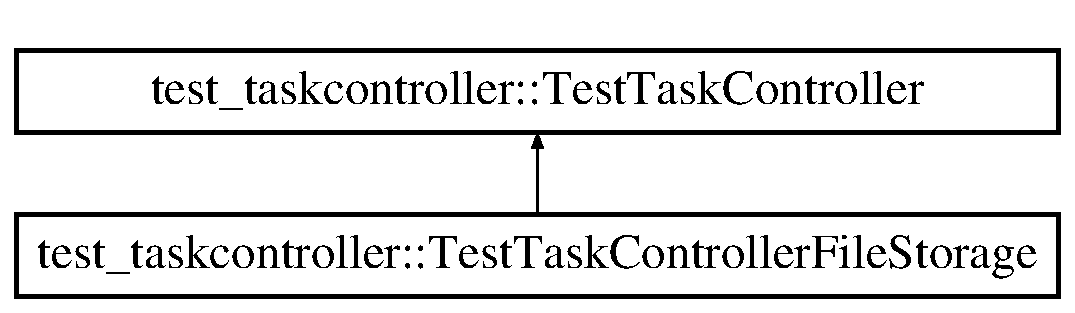
\includegraphics[height=2.000000cm]{classtest__taskcontroller_1_1TestTaskControllerFileStorage}
\end{center}
\end{figure}
\subsection*{\-Public \-Member \-Functions}
\begin{DoxyCompactItemize}
\item 
def \hyperlink{classtest__taskcontroller_1_1TestTaskControllerFileStorage_a1f63de1b9c566d073b4a11c5a49530c6}{\-\_\-\-\_\-init\-\_\-\-\_\-}
\item 
def \hyperlink{classtest__taskcontroller_1_1TestTaskControllerFileStorage_a6365fcf7e86a92beb75a3ba9295757e9}{set\-Up}
\item 
def \hyperlink{classtest__taskcontroller_1_1TestTaskControllerFileStorage_aaa88d65a1ecdd339726cc2fd67334743}{tear\-Down}
\end{DoxyCompactItemize}
\subsection*{\-Public \-Attributes}
\begin{DoxyCompactItemize}
\item 
\hyperlink{classtest__taskcontroller_1_1TestTaskControllerFileStorage_a049c3716a1d2a3c1e33c38eb654f15c9}{test\-\_\-task\-\_\-filename}
\item 
\hyperlink{classtest__taskcontroller_1_1TestTaskControllerFileStorage_adfb97b6e2fc6a47cc0da458781f256d6}{test\-\_\-key\-\_\-filename}
\item 
\hyperlink{classtest__taskcontroller_1_1TestTaskControllerFileStorage_acc2ab298aa1f3e5416310c8dfd118246}{interface\-\_\-controller}
\item 
\hyperlink{classtest__taskcontroller_1_1TestTaskControllerFileStorage_a4e8286cf16ac1c8751a710a36785aa69}{title}
\item 
\hyperlink{classtest__taskcontroller_1_1TestTaskControllerFileStorage_a6e7bbd4224d1fcff065cde59dbb651fc}{notes}
\item 
\hyperlink{classtest__taskcontroller_1_1TestTaskControllerFileStorage_ab690671055aca102212c66157ff1e246}{key}
\item 
\hyperlink{classtest__taskcontroller_1_1TestTaskControllerFileStorage_a5b9b16c50e8e488cbc066f5db85bca64}{added\-\_\-task}
\end{DoxyCompactItemize}


\subsection{\-Detailed \-Description}
\-Tests the \-Task\-Controller while using file storage. 

\-Definition at line 133 of file test\-\_\-taskcontroller.\-py.



\subsection{\-Constructor \& \-Destructor \-Documentation}
\hypertarget{classtest__taskcontroller_1_1TestTaskControllerFileStorage_a1f63de1b9c566d073b4a11c5a49530c6}{
\index{test\-\_\-taskcontroller\-::\-Test\-Task\-Controller\-File\-Storage@{test\-\_\-taskcontroller\-::\-Test\-Task\-Controller\-File\-Storage}!\-\_\-\-\_\-init\-\_\-\-\_\-@{\-\_\-\-\_\-init\-\_\-\-\_\-}}
\index{\-\_\-\-\_\-init\-\_\-\-\_\-@{\-\_\-\-\_\-init\-\_\-\-\_\-}!test_taskcontroller::TestTaskControllerFileStorage@{test\-\_\-taskcontroller\-::\-Test\-Task\-Controller\-File\-Storage}}
\subsubsection[{\-\_\-\-\_\-init\-\_\-\-\_\-}]{\setlength{\rightskip}{0pt plus 5cm}def test\-\_\-taskcontroller\-::\-Test\-Task\-Controller\-File\-Storage\-::\-\_\-\-\_\-init\-\_\-\-\_\- (
\begin{DoxyParamCaption}
\item[{}]{self, }
\item[{}]{method\-\_\-name}
\end{DoxyParamCaption}
)}}
\label{classtest__taskcontroller_1_1TestTaskControllerFileStorage_a1f63de1b9c566d073b4a11c5a49530c6}


\-Reimplemented from \hyperlink{classtest__taskcontroller_1_1TestTaskController_a2ec547bb413edbb40c0ae582dd2466bd}{test\-\_\-taskcontroller\-::\-Test\-Task\-Controller}.



\-Definition at line 135 of file test\-\_\-taskcontroller.\-py.



\subsection{\-Member \-Function \-Documentation}
\hypertarget{classtest__taskcontroller_1_1TestTaskControllerFileStorage_a6365fcf7e86a92beb75a3ba9295757e9}{
\index{test\-\_\-taskcontroller\-::\-Test\-Task\-Controller\-File\-Storage@{test\-\_\-taskcontroller\-::\-Test\-Task\-Controller\-File\-Storage}!set\-Up@{set\-Up}}
\index{set\-Up@{set\-Up}!test_taskcontroller::TestTaskControllerFileStorage@{test\-\_\-taskcontroller\-::\-Test\-Task\-Controller\-File\-Storage}}
\subsubsection[{set\-Up}]{\setlength{\rightskip}{0pt plus 5cm}def test\-\_\-taskcontroller\-::\-Test\-Task\-Controller\-File\-Storage\-::set\-Up (
\begin{DoxyParamCaption}
\item[{}]{self}
\end{DoxyParamCaption}
)}}
\label{classtest__taskcontroller_1_1TestTaskControllerFileStorage_a6365fcf7e86a92beb75a3ba9295757e9}


\-Definition at line 138 of file test\-\_\-taskcontroller.\-py.

\hypertarget{classtest__taskcontroller_1_1TestTaskControllerFileStorage_aaa88d65a1ecdd339726cc2fd67334743}{
\index{test\-\_\-taskcontroller\-::\-Test\-Task\-Controller\-File\-Storage@{test\-\_\-taskcontroller\-::\-Test\-Task\-Controller\-File\-Storage}!tear\-Down@{tear\-Down}}
\index{tear\-Down@{tear\-Down}!test_taskcontroller::TestTaskControllerFileStorage@{test\-\_\-taskcontroller\-::\-Test\-Task\-Controller\-File\-Storage}}
\subsubsection[{tear\-Down}]{\setlength{\rightskip}{0pt plus 5cm}def test\-\_\-taskcontroller\-::\-Test\-Task\-Controller\-File\-Storage\-::tear\-Down (
\begin{DoxyParamCaption}
\item[{}]{self}
\end{DoxyParamCaption}
)}}
\label{classtest__taskcontroller_1_1TestTaskControllerFileStorage_aaa88d65a1ecdd339726cc2fd67334743}


\-Definition at line 160 of file test\-\_\-taskcontroller.\-py.



\subsection{\-Member \-Data \-Documentation}
\hypertarget{classtest__taskcontroller_1_1TestTaskControllerFileStorage_a5b9b16c50e8e488cbc066f5db85bca64}{
\index{test\-\_\-taskcontroller\-::\-Test\-Task\-Controller\-File\-Storage@{test\-\_\-taskcontroller\-::\-Test\-Task\-Controller\-File\-Storage}!added\-\_\-task@{added\-\_\-task}}
\index{added\-\_\-task@{added\-\_\-task}!test_taskcontroller::TestTaskControllerFileStorage@{test\-\_\-taskcontroller\-::\-Test\-Task\-Controller\-File\-Storage}}
\subsubsection[{added\-\_\-task}]{\setlength{\rightskip}{0pt plus 5cm}{\bf test\-\_\-taskcontroller\-::\-Test\-Task\-Controller\-File\-Storage\-::added\-\_\-task}}}
\label{classtest__taskcontroller_1_1TestTaskControllerFileStorage_a5b9b16c50e8e488cbc066f5db85bca64}


\-Reimplemented from \hyperlink{classtest__taskcontroller_1_1TestTaskController_a8b748405763b73406ca9cfafe467c0a1}{test\-\_\-taskcontroller\-::\-Test\-Task\-Controller}.



\-Definition at line 138 of file test\-\_\-taskcontroller.\-py.

\hypertarget{classtest__taskcontroller_1_1TestTaskControllerFileStorage_acc2ab298aa1f3e5416310c8dfd118246}{
\index{test\-\_\-taskcontroller\-::\-Test\-Task\-Controller\-File\-Storage@{test\-\_\-taskcontroller\-::\-Test\-Task\-Controller\-File\-Storage}!interface\-\_\-controller@{interface\-\_\-controller}}
\index{interface\-\_\-controller@{interface\-\_\-controller}!test_taskcontroller::TestTaskControllerFileStorage@{test\-\_\-taskcontroller\-::\-Test\-Task\-Controller\-File\-Storage}}
\subsubsection[{interface\-\_\-controller}]{\setlength{\rightskip}{0pt plus 5cm}{\bf test\-\_\-taskcontroller\-::\-Test\-Task\-Controller\-File\-Storage\-::interface\-\_\-controller}}}
\label{classtest__taskcontroller_1_1TestTaskControllerFileStorage_acc2ab298aa1f3e5416310c8dfd118246}


\-Reimplemented from \hyperlink{classtest__taskcontroller_1_1TestTaskController_a16cbd17e4ad8bf93e164813b77313942}{test\-\_\-taskcontroller\-::\-Test\-Task\-Controller}.



\-Definition at line 138 of file test\-\_\-taskcontroller.\-py.

\hypertarget{classtest__taskcontroller_1_1TestTaskControllerFileStorage_ab690671055aca102212c66157ff1e246}{
\index{test\-\_\-taskcontroller\-::\-Test\-Task\-Controller\-File\-Storage@{test\-\_\-taskcontroller\-::\-Test\-Task\-Controller\-File\-Storage}!key@{key}}
\index{key@{key}!test_taskcontroller::TestTaskControllerFileStorage@{test\-\_\-taskcontroller\-::\-Test\-Task\-Controller\-File\-Storage}}
\subsubsection[{key}]{\setlength{\rightskip}{0pt plus 5cm}{\bf test\-\_\-taskcontroller\-::\-Test\-Task\-Controller\-File\-Storage\-::key}}}
\label{classtest__taskcontroller_1_1TestTaskControllerFileStorage_ab690671055aca102212c66157ff1e246}


\-Definition at line 138 of file test\-\_\-taskcontroller.\-py.

\hypertarget{classtest__taskcontroller_1_1TestTaskControllerFileStorage_a6e7bbd4224d1fcff065cde59dbb651fc}{
\index{test\-\_\-taskcontroller\-::\-Test\-Task\-Controller\-File\-Storage@{test\-\_\-taskcontroller\-::\-Test\-Task\-Controller\-File\-Storage}!notes@{notes}}
\index{notes@{notes}!test_taskcontroller::TestTaskControllerFileStorage@{test\-\_\-taskcontroller\-::\-Test\-Task\-Controller\-File\-Storage}}
\subsubsection[{notes}]{\setlength{\rightskip}{0pt plus 5cm}{\bf test\-\_\-taskcontroller\-::\-Test\-Task\-Controller\-File\-Storage\-::notes}}}
\label{classtest__taskcontroller_1_1TestTaskControllerFileStorage_a6e7bbd4224d1fcff065cde59dbb651fc}


\-Reimplemented from \hyperlink{classtest__taskcontroller_1_1TestTaskController_a9825f47dfebf3e25f03548d51d1d07d1}{test\-\_\-taskcontroller\-::\-Test\-Task\-Controller}.



\-Definition at line 138 of file test\-\_\-taskcontroller.\-py.

\hypertarget{classtest__taskcontroller_1_1TestTaskControllerFileStorage_adfb97b6e2fc6a47cc0da458781f256d6}{
\index{test\-\_\-taskcontroller\-::\-Test\-Task\-Controller\-File\-Storage@{test\-\_\-taskcontroller\-::\-Test\-Task\-Controller\-File\-Storage}!test\-\_\-key\-\_\-filename@{test\-\_\-key\-\_\-filename}}
\index{test\-\_\-key\-\_\-filename@{test\-\_\-key\-\_\-filename}!test_taskcontroller::TestTaskControllerFileStorage@{test\-\_\-taskcontroller\-::\-Test\-Task\-Controller\-File\-Storage}}
\subsubsection[{test\-\_\-key\-\_\-filename}]{\setlength{\rightskip}{0pt plus 5cm}{\bf test\-\_\-taskcontroller\-::\-Test\-Task\-Controller\-File\-Storage\-::test\-\_\-key\-\_\-filename}}}
\label{classtest__taskcontroller_1_1TestTaskControllerFileStorage_adfb97b6e2fc6a47cc0da458781f256d6}


\-Definition at line 138 of file test\-\_\-taskcontroller.\-py.

\hypertarget{classtest__taskcontroller_1_1TestTaskControllerFileStorage_a049c3716a1d2a3c1e33c38eb654f15c9}{
\index{test\-\_\-taskcontroller\-::\-Test\-Task\-Controller\-File\-Storage@{test\-\_\-taskcontroller\-::\-Test\-Task\-Controller\-File\-Storage}!test\-\_\-task\-\_\-filename@{test\-\_\-task\-\_\-filename}}
\index{test\-\_\-task\-\_\-filename@{test\-\_\-task\-\_\-filename}!test_taskcontroller::TestTaskControllerFileStorage@{test\-\_\-taskcontroller\-::\-Test\-Task\-Controller\-File\-Storage}}
\subsubsection[{test\-\_\-task\-\_\-filename}]{\setlength{\rightskip}{0pt plus 5cm}{\bf test\-\_\-taskcontroller\-::\-Test\-Task\-Controller\-File\-Storage\-::test\-\_\-task\-\_\-filename}}}
\label{classtest__taskcontroller_1_1TestTaskControllerFileStorage_a049c3716a1d2a3c1e33c38eb654f15c9}


\-Definition at line 138 of file test\-\_\-taskcontroller.\-py.

\hypertarget{classtest__taskcontroller_1_1TestTaskControllerFileStorage_a4e8286cf16ac1c8751a710a36785aa69}{
\index{test\-\_\-taskcontroller\-::\-Test\-Task\-Controller\-File\-Storage@{test\-\_\-taskcontroller\-::\-Test\-Task\-Controller\-File\-Storage}!title@{title}}
\index{title@{title}!test_taskcontroller::TestTaskControllerFileStorage@{test\-\_\-taskcontroller\-::\-Test\-Task\-Controller\-File\-Storage}}
\subsubsection[{title}]{\setlength{\rightskip}{0pt plus 5cm}{\bf test\-\_\-taskcontroller\-::\-Test\-Task\-Controller\-File\-Storage\-::title}}}
\label{classtest__taskcontroller_1_1TestTaskControllerFileStorage_a4e8286cf16ac1c8751a710a36785aa69}


\-Reimplemented from \hyperlink{classtest__taskcontroller_1_1TestTaskController_a450431cde03f14169cd5ac04db704ab6}{test\-\_\-taskcontroller\-::\-Test\-Task\-Controller}.



\-Definition at line 138 of file test\-\_\-taskcontroller.\-py.



\-The documentation for this class was generated from the following file\-:\begin{DoxyCompactItemize}
\item 
/home/scott/school/capstone/\-Task-\/\-Organizer/src/test/\hyperlink{test__taskcontroller_8py}{test\-\_\-taskcontroller.\-py}\end{DoxyCompactItemize}

\hypertarget{classtest__taskcontroller_1_1TestTaskControllerGTaskStorage}{
\section{test\-\_\-taskcontroller\-:\-:\-Test\-Task\-Controller\-G\-Task\-Storage \-Class \-Reference}
\label{classtest__taskcontroller_1_1TestTaskControllerGTaskStorage}\index{test\-\_\-taskcontroller\-::\-Test\-Task\-Controller\-G\-Task\-Storage@{test\-\_\-taskcontroller\-::\-Test\-Task\-Controller\-G\-Task\-Storage}}
}


\-Tests the \-Task\-Controller while using \-G\-Task storage.  


\-Inheritance diagram for test\-\_\-taskcontroller\-:\-:\-Test\-Task\-Controller\-G\-Task\-Storage\-:\begin{figure}[H]
\begin{center}
\leavevmode
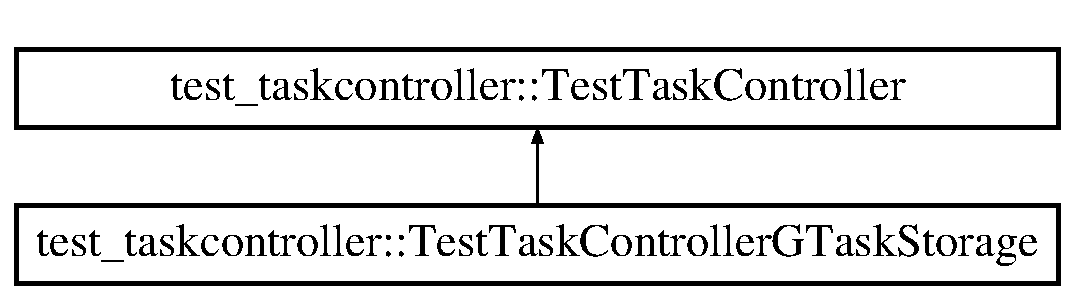
\includegraphics[height=2.000000cm]{classtest__taskcontroller_1_1TestTaskControllerGTaskStorage}
\end{center}
\end{figure}
\subsection*{\-Public \-Member \-Functions}
\begin{DoxyCompactItemize}
\item 
def \hyperlink{classtest__taskcontroller_1_1TestTaskControllerGTaskStorage_a6486ee999987082360633f99b887af86}{\-\_\-\-\_\-init\-\_\-\-\_\-}
\item 
def \hyperlink{classtest__taskcontroller_1_1TestTaskControllerGTaskStorage_a303ff45836c0c66b699198f28e175919}{set\-Up}
\item 
def \hyperlink{classtest__taskcontroller_1_1TestTaskControllerGTaskStorage_aec5a09686478b70dfc45ce1bb8d22391}{tear\-Down}
\end{DoxyCompactItemize}
\subsection*{\-Public \-Attributes}
\begin{DoxyCompactItemize}
\item 
\hyperlink{classtest__taskcontroller_1_1TestTaskControllerGTaskStorage_ac6b50d155cf6a1b6e013aec3b5239506}{interface\-\_\-controller}
\item 
\hyperlink{classtest__taskcontroller_1_1TestTaskControllerGTaskStorage_afac8474c0938bce8e9ffa5c809d65e7a}{title}
\item 
\hyperlink{classtest__taskcontroller_1_1TestTaskControllerGTaskStorage_af68b73d943db052577719cfc4c1cebbf}{notes}
\item 
\hyperlink{classtest__taskcontroller_1_1TestTaskControllerGTaskStorage_a35c627557770a4afdf881f16ac42b16a}{key}
\item 
\hyperlink{classtest__taskcontroller_1_1TestTaskControllerGTaskStorage_a150fa26a41cdce7d5d753edf43d5a09e}{added\-\_\-task}
\end{DoxyCompactItemize}


\subsection{\-Detailed \-Description}
\-Tests the \-Task\-Controller while using \-G\-Task storage. 

\-Definition at line 193 of file test\-\_\-taskcontroller.\-py.



\subsection{\-Constructor \& \-Destructor \-Documentation}
\hypertarget{classtest__taskcontroller_1_1TestTaskControllerGTaskStorage_a6486ee999987082360633f99b887af86}{
\index{test\-\_\-taskcontroller\-::\-Test\-Task\-Controller\-G\-Task\-Storage@{test\-\_\-taskcontroller\-::\-Test\-Task\-Controller\-G\-Task\-Storage}!\-\_\-\-\_\-init\-\_\-\-\_\-@{\-\_\-\-\_\-init\-\_\-\-\_\-}}
\index{\-\_\-\-\_\-init\-\_\-\-\_\-@{\-\_\-\-\_\-init\-\_\-\-\_\-}!test_taskcontroller::TestTaskControllerGTaskStorage@{test\-\_\-taskcontroller\-::\-Test\-Task\-Controller\-G\-Task\-Storage}}
\subsubsection[{\-\_\-\-\_\-init\-\_\-\-\_\-}]{\setlength{\rightskip}{0pt plus 5cm}def test\-\_\-taskcontroller\-::\-Test\-Task\-Controller\-G\-Task\-Storage\-::\-\_\-\-\_\-init\-\_\-\-\_\- (
\begin{DoxyParamCaption}
\item[{}]{self, }
\item[{}]{method\-\_\-name}
\end{DoxyParamCaption}
)}}
\label{classtest__taskcontroller_1_1TestTaskControllerGTaskStorage_a6486ee999987082360633f99b887af86}


\-Reimplemented from \hyperlink{classtest__taskcontroller_1_1TestTaskController_a2ec547bb413edbb40c0ae582dd2466bd}{test\-\_\-taskcontroller\-::\-Test\-Task\-Controller}.



\-Definition at line 195 of file test\-\_\-taskcontroller.\-py.



\subsection{\-Member \-Function \-Documentation}
\hypertarget{classtest__taskcontroller_1_1TestTaskControllerGTaskStorage_a303ff45836c0c66b699198f28e175919}{
\index{test\-\_\-taskcontroller\-::\-Test\-Task\-Controller\-G\-Task\-Storage@{test\-\_\-taskcontroller\-::\-Test\-Task\-Controller\-G\-Task\-Storage}!set\-Up@{set\-Up}}
\index{set\-Up@{set\-Up}!test_taskcontroller::TestTaskControllerGTaskStorage@{test\-\_\-taskcontroller\-::\-Test\-Task\-Controller\-G\-Task\-Storage}}
\subsubsection[{set\-Up}]{\setlength{\rightskip}{0pt plus 5cm}def test\-\_\-taskcontroller\-::\-Test\-Task\-Controller\-G\-Task\-Storage\-::set\-Up (
\begin{DoxyParamCaption}
\item[{}]{self}
\end{DoxyParamCaption}
)}}
\label{classtest__taskcontroller_1_1TestTaskControllerGTaskStorage_a303ff45836c0c66b699198f28e175919}


\-Definition at line 198 of file test\-\_\-taskcontroller.\-py.

\hypertarget{classtest__taskcontroller_1_1TestTaskControllerGTaskStorage_aec5a09686478b70dfc45ce1bb8d22391}{
\index{test\-\_\-taskcontroller\-::\-Test\-Task\-Controller\-G\-Task\-Storage@{test\-\_\-taskcontroller\-::\-Test\-Task\-Controller\-G\-Task\-Storage}!tear\-Down@{tear\-Down}}
\index{tear\-Down@{tear\-Down}!test_taskcontroller::TestTaskControllerGTaskStorage@{test\-\_\-taskcontroller\-::\-Test\-Task\-Controller\-G\-Task\-Storage}}
\subsubsection[{tear\-Down}]{\setlength{\rightskip}{0pt plus 5cm}def test\-\_\-taskcontroller\-::\-Test\-Task\-Controller\-G\-Task\-Storage\-::tear\-Down (
\begin{DoxyParamCaption}
\item[{}]{self}
\end{DoxyParamCaption}
)}}
\label{classtest__taskcontroller_1_1TestTaskControllerGTaskStorage_aec5a09686478b70dfc45ce1bb8d22391}


\-Definition at line 211 of file test\-\_\-taskcontroller.\-py.



\subsection{\-Member \-Data \-Documentation}
\hypertarget{classtest__taskcontroller_1_1TestTaskControllerGTaskStorage_a150fa26a41cdce7d5d753edf43d5a09e}{
\index{test\-\_\-taskcontroller\-::\-Test\-Task\-Controller\-G\-Task\-Storage@{test\-\_\-taskcontroller\-::\-Test\-Task\-Controller\-G\-Task\-Storage}!added\-\_\-task@{added\-\_\-task}}
\index{added\-\_\-task@{added\-\_\-task}!test_taskcontroller::TestTaskControllerGTaskStorage@{test\-\_\-taskcontroller\-::\-Test\-Task\-Controller\-G\-Task\-Storage}}
\subsubsection[{added\-\_\-task}]{\setlength{\rightskip}{0pt plus 5cm}{\bf test\-\_\-taskcontroller\-::\-Test\-Task\-Controller\-G\-Task\-Storage\-::added\-\_\-task}}}
\label{classtest__taskcontroller_1_1TestTaskControllerGTaskStorage_a150fa26a41cdce7d5d753edf43d5a09e}


\-Reimplemented from \hyperlink{classtest__taskcontroller_1_1TestTaskController_a8b748405763b73406ca9cfafe467c0a1}{test\-\_\-taskcontroller\-::\-Test\-Task\-Controller}.



\-Definition at line 198 of file test\-\_\-taskcontroller.\-py.

\hypertarget{classtest__taskcontroller_1_1TestTaskControllerGTaskStorage_ac6b50d155cf6a1b6e013aec3b5239506}{
\index{test\-\_\-taskcontroller\-::\-Test\-Task\-Controller\-G\-Task\-Storage@{test\-\_\-taskcontroller\-::\-Test\-Task\-Controller\-G\-Task\-Storage}!interface\-\_\-controller@{interface\-\_\-controller}}
\index{interface\-\_\-controller@{interface\-\_\-controller}!test_taskcontroller::TestTaskControllerGTaskStorage@{test\-\_\-taskcontroller\-::\-Test\-Task\-Controller\-G\-Task\-Storage}}
\subsubsection[{interface\-\_\-controller}]{\setlength{\rightskip}{0pt plus 5cm}{\bf test\-\_\-taskcontroller\-::\-Test\-Task\-Controller\-G\-Task\-Storage\-::interface\-\_\-controller}}}
\label{classtest__taskcontroller_1_1TestTaskControllerGTaskStorage_ac6b50d155cf6a1b6e013aec3b5239506}


\-Reimplemented from \hyperlink{classtest__taskcontroller_1_1TestTaskController_a16cbd17e4ad8bf93e164813b77313942}{test\-\_\-taskcontroller\-::\-Test\-Task\-Controller}.



\-Definition at line 198 of file test\-\_\-taskcontroller.\-py.

\hypertarget{classtest__taskcontroller_1_1TestTaskControllerGTaskStorage_a35c627557770a4afdf881f16ac42b16a}{
\index{test\-\_\-taskcontroller\-::\-Test\-Task\-Controller\-G\-Task\-Storage@{test\-\_\-taskcontroller\-::\-Test\-Task\-Controller\-G\-Task\-Storage}!key@{key}}
\index{key@{key}!test_taskcontroller::TestTaskControllerGTaskStorage@{test\-\_\-taskcontroller\-::\-Test\-Task\-Controller\-G\-Task\-Storage}}
\subsubsection[{key}]{\setlength{\rightskip}{0pt plus 5cm}{\bf test\-\_\-taskcontroller\-::\-Test\-Task\-Controller\-G\-Task\-Storage\-::key}}}
\label{classtest__taskcontroller_1_1TestTaskControllerGTaskStorage_a35c627557770a4afdf881f16ac42b16a}


\-Definition at line 198 of file test\-\_\-taskcontroller.\-py.

\hypertarget{classtest__taskcontroller_1_1TestTaskControllerGTaskStorage_af68b73d943db052577719cfc4c1cebbf}{
\index{test\-\_\-taskcontroller\-::\-Test\-Task\-Controller\-G\-Task\-Storage@{test\-\_\-taskcontroller\-::\-Test\-Task\-Controller\-G\-Task\-Storage}!notes@{notes}}
\index{notes@{notes}!test_taskcontroller::TestTaskControllerGTaskStorage@{test\-\_\-taskcontroller\-::\-Test\-Task\-Controller\-G\-Task\-Storage}}
\subsubsection[{notes}]{\setlength{\rightskip}{0pt plus 5cm}{\bf test\-\_\-taskcontroller\-::\-Test\-Task\-Controller\-G\-Task\-Storage\-::notes}}}
\label{classtest__taskcontroller_1_1TestTaskControllerGTaskStorage_af68b73d943db052577719cfc4c1cebbf}


\-Reimplemented from \hyperlink{classtest__taskcontroller_1_1TestTaskController_a9825f47dfebf3e25f03548d51d1d07d1}{test\-\_\-taskcontroller\-::\-Test\-Task\-Controller}.



\-Definition at line 198 of file test\-\_\-taskcontroller.\-py.

\hypertarget{classtest__taskcontroller_1_1TestTaskControllerGTaskStorage_afac8474c0938bce8e9ffa5c809d65e7a}{
\index{test\-\_\-taskcontroller\-::\-Test\-Task\-Controller\-G\-Task\-Storage@{test\-\_\-taskcontroller\-::\-Test\-Task\-Controller\-G\-Task\-Storage}!title@{title}}
\index{title@{title}!test_taskcontroller::TestTaskControllerGTaskStorage@{test\-\_\-taskcontroller\-::\-Test\-Task\-Controller\-G\-Task\-Storage}}
\subsubsection[{title}]{\setlength{\rightskip}{0pt plus 5cm}{\bf test\-\_\-taskcontroller\-::\-Test\-Task\-Controller\-G\-Task\-Storage\-::title}}}
\label{classtest__taskcontroller_1_1TestTaskControllerGTaskStorage_afac8474c0938bce8e9ffa5c809d65e7a}


\-Reimplemented from \hyperlink{classtest__taskcontroller_1_1TestTaskController_a450431cde03f14169cd5ac04db704ab6}{test\-\_\-taskcontroller\-::\-Test\-Task\-Controller}.



\-Definition at line 198 of file test\-\_\-taskcontroller.\-py.



\-The documentation for this class was generated from the following file\-:\begin{DoxyCompactItemize}
\item 
/home/scott/school/capstone/\-Task-\/\-Organizer/src/test/\hyperlink{test__taskcontroller_8py}{test\-\_\-taskcontroller.\-py}\end{DoxyCompactItemize}

\hypertarget{classtest__taskcontroller_1_1TestTaskControllerSQLiteStorage}{
\section{test\-\_\-taskcontroller\-:\-:\-Test\-Task\-Controller\-S\-Q\-Lite\-Storage \-Class \-Reference}
\label{classtest__taskcontroller_1_1TestTaskControllerSQLiteStorage}\index{test\-\_\-taskcontroller\-::\-Test\-Task\-Controller\-S\-Q\-Lite\-Storage@{test\-\_\-taskcontroller\-::\-Test\-Task\-Controller\-S\-Q\-Lite\-Storage}}
}


\-Tests the \-Task\-Controller while using sqlite storage.  


\-Inheritance diagram for test\-\_\-taskcontroller\-:\-:\-Test\-Task\-Controller\-S\-Q\-Lite\-Storage\-:\begin{figure}[H]
\begin{center}
\leavevmode
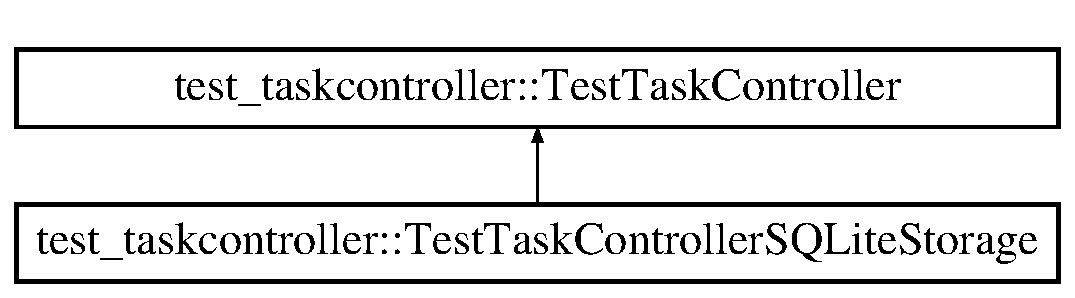
\includegraphics[height=2.000000cm]{classtest__taskcontroller_1_1TestTaskControllerSQLiteStorage}
\end{center}
\end{figure}
\subsection*{\-Public \-Member \-Functions}
\begin{DoxyCompactItemize}
\item 
def \hyperlink{classtest__taskcontroller_1_1TestTaskControllerSQLiteStorage_a29417d2c4aee8c9bd135faff67203edc}{\-\_\-\-\_\-init\-\_\-\-\_\-}
\item 
def \hyperlink{classtest__taskcontroller_1_1TestTaskControllerSQLiteStorage_af9e2857d37a141eefd0fa801d22d2666}{set\-Up}
\item 
def \hyperlink{classtest__taskcontroller_1_1TestTaskControllerSQLiteStorage_ae9e702f3aa351b7f2f6a46fab57af8be}{tear\-Down}
\end{DoxyCompactItemize}
\subsection*{\-Public \-Attributes}
\begin{DoxyCompactItemize}
\item 
\hyperlink{classtest__taskcontroller_1_1TestTaskControllerSQLiteStorage_abb0b790c54971a3e9ab953488e29a848}{test\-\_\-task\-\_\-dbname}
\item 
\hyperlink{classtest__taskcontroller_1_1TestTaskControllerSQLiteStorage_a57793e2bedf041d117057533c98ecc48}{interface\-\_\-controller}
\item 
\hyperlink{classtest__taskcontroller_1_1TestTaskControllerSQLiteStorage_a3fcf0960dcbb4eb0c910638fc6789480}{title}
\item 
\hyperlink{classtest__taskcontroller_1_1TestTaskControllerSQLiteStorage_a5ddf73f3d29305c397092befa1063493}{notes}
\item 
\hyperlink{classtest__taskcontroller_1_1TestTaskControllerSQLiteStorage_a193d1ef890fde41f33876d67fe8c4093}{key}
\item 
\hyperlink{classtest__taskcontroller_1_1TestTaskControllerSQLiteStorage_aa69b7c38504f5c50040bec6b0fcc73c3}{added\-\_\-task}
\end{DoxyCompactItemize}


\subsection{\-Detailed \-Description}
\-Tests the \-Task\-Controller while using sqlite storage. 

\-Definition at line 167 of file test\-\_\-taskcontroller.\-py.



\subsection{\-Constructor \& \-Destructor \-Documentation}
\hypertarget{classtest__taskcontroller_1_1TestTaskControllerSQLiteStorage_a29417d2c4aee8c9bd135faff67203edc}{
\index{test\-\_\-taskcontroller\-::\-Test\-Task\-Controller\-S\-Q\-Lite\-Storage@{test\-\_\-taskcontroller\-::\-Test\-Task\-Controller\-S\-Q\-Lite\-Storage}!\-\_\-\-\_\-init\-\_\-\-\_\-@{\-\_\-\-\_\-init\-\_\-\-\_\-}}
\index{\-\_\-\-\_\-init\-\_\-\-\_\-@{\-\_\-\-\_\-init\-\_\-\-\_\-}!test_taskcontroller::TestTaskControllerSQLiteStorage@{test\-\_\-taskcontroller\-::\-Test\-Task\-Controller\-S\-Q\-Lite\-Storage}}
\subsubsection[{\-\_\-\-\_\-init\-\_\-\-\_\-}]{\setlength{\rightskip}{0pt plus 5cm}def test\-\_\-taskcontroller\-::\-Test\-Task\-Controller\-S\-Q\-Lite\-Storage\-::\-\_\-\-\_\-init\-\_\-\-\_\- (
\begin{DoxyParamCaption}
\item[{}]{self, }
\item[{}]{method\-\_\-name}
\end{DoxyParamCaption}
)}}
\label{classtest__taskcontroller_1_1TestTaskControllerSQLiteStorage_a29417d2c4aee8c9bd135faff67203edc}


\-Reimplemented from \hyperlink{classtest__taskcontroller_1_1TestTaskController_a2ec547bb413edbb40c0ae582dd2466bd}{test\-\_\-taskcontroller\-::\-Test\-Task\-Controller}.



\-Definition at line 169 of file test\-\_\-taskcontroller.\-py.



\subsection{\-Member \-Function \-Documentation}
\hypertarget{classtest__taskcontroller_1_1TestTaskControllerSQLiteStorage_af9e2857d37a141eefd0fa801d22d2666}{
\index{test\-\_\-taskcontroller\-::\-Test\-Task\-Controller\-S\-Q\-Lite\-Storage@{test\-\_\-taskcontroller\-::\-Test\-Task\-Controller\-S\-Q\-Lite\-Storage}!set\-Up@{set\-Up}}
\index{set\-Up@{set\-Up}!test_taskcontroller::TestTaskControllerSQLiteStorage@{test\-\_\-taskcontroller\-::\-Test\-Task\-Controller\-S\-Q\-Lite\-Storage}}
\subsubsection[{set\-Up}]{\setlength{\rightskip}{0pt plus 5cm}def test\-\_\-taskcontroller\-::\-Test\-Task\-Controller\-S\-Q\-Lite\-Storage\-::set\-Up (
\begin{DoxyParamCaption}
\item[{}]{self}
\end{DoxyParamCaption}
)}}
\label{classtest__taskcontroller_1_1TestTaskControllerSQLiteStorage_af9e2857d37a141eefd0fa801d22d2666}


\-Definition at line 172 of file test\-\_\-taskcontroller.\-py.

\hypertarget{classtest__taskcontroller_1_1TestTaskControllerSQLiteStorage_ae9e702f3aa351b7f2f6a46fab57af8be}{
\index{test\-\_\-taskcontroller\-::\-Test\-Task\-Controller\-S\-Q\-Lite\-Storage@{test\-\_\-taskcontroller\-::\-Test\-Task\-Controller\-S\-Q\-Lite\-Storage}!tear\-Down@{tear\-Down}}
\index{tear\-Down@{tear\-Down}!test_taskcontroller::TestTaskControllerSQLiteStorage@{test\-\_\-taskcontroller\-::\-Test\-Task\-Controller\-S\-Q\-Lite\-Storage}}
\subsubsection[{tear\-Down}]{\setlength{\rightskip}{0pt plus 5cm}def test\-\_\-taskcontroller\-::\-Test\-Task\-Controller\-S\-Q\-Lite\-Storage\-::tear\-Down (
\begin{DoxyParamCaption}
\item[{}]{self}
\end{DoxyParamCaption}
)}}
\label{classtest__taskcontroller_1_1TestTaskControllerSQLiteStorage_ae9e702f3aa351b7f2f6a46fab57af8be}


\-Definition at line 187 of file test\-\_\-taskcontroller.\-py.



\subsection{\-Member \-Data \-Documentation}
\hypertarget{classtest__taskcontroller_1_1TestTaskControllerSQLiteStorage_aa69b7c38504f5c50040bec6b0fcc73c3}{
\index{test\-\_\-taskcontroller\-::\-Test\-Task\-Controller\-S\-Q\-Lite\-Storage@{test\-\_\-taskcontroller\-::\-Test\-Task\-Controller\-S\-Q\-Lite\-Storage}!added\-\_\-task@{added\-\_\-task}}
\index{added\-\_\-task@{added\-\_\-task}!test_taskcontroller::TestTaskControllerSQLiteStorage@{test\-\_\-taskcontroller\-::\-Test\-Task\-Controller\-S\-Q\-Lite\-Storage}}
\subsubsection[{added\-\_\-task}]{\setlength{\rightskip}{0pt plus 5cm}{\bf test\-\_\-taskcontroller\-::\-Test\-Task\-Controller\-S\-Q\-Lite\-Storage\-::added\-\_\-task}}}
\label{classtest__taskcontroller_1_1TestTaskControllerSQLiteStorage_aa69b7c38504f5c50040bec6b0fcc73c3}


\-Reimplemented from \hyperlink{classtest__taskcontroller_1_1TestTaskController_a8b748405763b73406ca9cfafe467c0a1}{test\-\_\-taskcontroller\-::\-Test\-Task\-Controller}.



\-Definition at line 172 of file test\-\_\-taskcontroller.\-py.

\hypertarget{classtest__taskcontroller_1_1TestTaskControllerSQLiteStorage_a57793e2bedf041d117057533c98ecc48}{
\index{test\-\_\-taskcontroller\-::\-Test\-Task\-Controller\-S\-Q\-Lite\-Storage@{test\-\_\-taskcontroller\-::\-Test\-Task\-Controller\-S\-Q\-Lite\-Storage}!interface\-\_\-controller@{interface\-\_\-controller}}
\index{interface\-\_\-controller@{interface\-\_\-controller}!test_taskcontroller::TestTaskControllerSQLiteStorage@{test\-\_\-taskcontroller\-::\-Test\-Task\-Controller\-S\-Q\-Lite\-Storage}}
\subsubsection[{interface\-\_\-controller}]{\setlength{\rightskip}{0pt plus 5cm}{\bf test\-\_\-taskcontroller\-::\-Test\-Task\-Controller\-S\-Q\-Lite\-Storage\-::interface\-\_\-controller}}}
\label{classtest__taskcontroller_1_1TestTaskControllerSQLiteStorage_a57793e2bedf041d117057533c98ecc48}


\-Reimplemented from \hyperlink{classtest__taskcontroller_1_1TestTaskController_a16cbd17e4ad8bf93e164813b77313942}{test\-\_\-taskcontroller\-::\-Test\-Task\-Controller}.



\-Definition at line 172 of file test\-\_\-taskcontroller.\-py.

\hypertarget{classtest__taskcontroller_1_1TestTaskControllerSQLiteStorage_a193d1ef890fde41f33876d67fe8c4093}{
\index{test\-\_\-taskcontroller\-::\-Test\-Task\-Controller\-S\-Q\-Lite\-Storage@{test\-\_\-taskcontroller\-::\-Test\-Task\-Controller\-S\-Q\-Lite\-Storage}!key@{key}}
\index{key@{key}!test_taskcontroller::TestTaskControllerSQLiteStorage@{test\-\_\-taskcontroller\-::\-Test\-Task\-Controller\-S\-Q\-Lite\-Storage}}
\subsubsection[{key}]{\setlength{\rightskip}{0pt plus 5cm}{\bf test\-\_\-taskcontroller\-::\-Test\-Task\-Controller\-S\-Q\-Lite\-Storage\-::key}}}
\label{classtest__taskcontroller_1_1TestTaskControllerSQLiteStorage_a193d1ef890fde41f33876d67fe8c4093}


\-Definition at line 172 of file test\-\_\-taskcontroller.\-py.

\hypertarget{classtest__taskcontroller_1_1TestTaskControllerSQLiteStorage_a5ddf73f3d29305c397092befa1063493}{
\index{test\-\_\-taskcontroller\-::\-Test\-Task\-Controller\-S\-Q\-Lite\-Storage@{test\-\_\-taskcontroller\-::\-Test\-Task\-Controller\-S\-Q\-Lite\-Storage}!notes@{notes}}
\index{notes@{notes}!test_taskcontroller::TestTaskControllerSQLiteStorage@{test\-\_\-taskcontroller\-::\-Test\-Task\-Controller\-S\-Q\-Lite\-Storage}}
\subsubsection[{notes}]{\setlength{\rightskip}{0pt plus 5cm}{\bf test\-\_\-taskcontroller\-::\-Test\-Task\-Controller\-S\-Q\-Lite\-Storage\-::notes}}}
\label{classtest__taskcontroller_1_1TestTaskControllerSQLiteStorage_a5ddf73f3d29305c397092befa1063493}


\-Reimplemented from \hyperlink{classtest__taskcontroller_1_1TestTaskController_a9825f47dfebf3e25f03548d51d1d07d1}{test\-\_\-taskcontroller\-::\-Test\-Task\-Controller}.



\-Definition at line 172 of file test\-\_\-taskcontroller.\-py.

\hypertarget{classtest__taskcontroller_1_1TestTaskControllerSQLiteStorage_abb0b790c54971a3e9ab953488e29a848}{
\index{test\-\_\-taskcontroller\-::\-Test\-Task\-Controller\-S\-Q\-Lite\-Storage@{test\-\_\-taskcontroller\-::\-Test\-Task\-Controller\-S\-Q\-Lite\-Storage}!test\-\_\-task\-\_\-dbname@{test\-\_\-task\-\_\-dbname}}
\index{test\-\_\-task\-\_\-dbname@{test\-\_\-task\-\_\-dbname}!test_taskcontroller::TestTaskControllerSQLiteStorage@{test\-\_\-taskcontroller\-::\-Test\-Task\-Controller\-S\-Q\-Lite\-Storage}}
\subsubsection[{test\-\_\-task\-\_\-dbname}]{\setlength{\rightskip}{0pt plus 5cm}{\bf test\-\_\-taskcontroller\-::\-Test\-Task\-Controller\-S\-Q\-Lite\-Storage\-::test\-\_\-task\-\_\-dbname}}}
\label{classtest__taskcontroller_1_1TestTaskControllerSQLiteStorage_abb0b790c54971a3e9ab953488e29a848}


\-Definition at line 172 of file test\-\_\-taskcontroller.\-py.

\hypertarget{classtest__taskcontroller_1_1TestTaskControllerSQLiteStorage_a3fcf0960dcbb4eb0c910638fc6789480}{
\index{test\-\_\-taskcontroller\-::\-Test\-Task\-Controller\-S\-Q\-Lite\-Storage@{test\-\_\-taskcontroller\-::\-Test\-Task\-Controller\-S\-Q\-Lite\-Storage}!title@{title}}
\index{title@{title}!test_taskcontroller::TestTaskControllerSQLiteStorage@{test\-\_\-taskcontroller\-::\-Test\-Task\-Controller\-S\-Q\-Lite\-Storage}}
\subsubsection[{title}]{\setlength{\rightskip}{0pt plus 5cm}{\bf test\-\_\-taskcontroller\-::\-Test\-Task\-Controller\-S\-Q\-Lite\-Storage\-::title}}}
\label{classtest__taskcontroller_1_1TestTaskControllerSQLiteStorage_a3fcf0960dcbb4eb0c910638fc6789480}


\-Reimplemented from \hyperlink{classtest__taskcontroller_1_1TestTaskController_a450431cde03f14169cd5ac04db704ab6}{test\-\_\-taskcontroller\-::\-Test\-Task\-Controller}.



\-Definition at line 172 of file test\-\_\-taskcontroller.\-py.



\-The documentation for this class was generated from the following file\-:\begin{DoxyCompactItemize}
\item 
/home/scott/school/capstone/\-Task-\/\-Organizer/src/test/\hyperlink{test__taskcontroller_8py}{test\-\_\-taskcontroller.\-py}\end{DoxyCompactItemize}

\hypertarget{classtest__task_1_1TestTaskCreator}{
\section{test\-\_\-task\-:\-:\-Test\-Task\-Creator \-Class \-Reference}
\label{classtest__task_1_1TestTaskCreator}\index{test\-\_\-task\-::\-Test\-Task\-Creator@{test\-\_\-task\-::\-Test\-Task\-Creator}}
}


\-Tests that \-Task\-Creator correctly creates \-Task objects.  


\subsection*{\-Public \-Member \-Functions}
\begin{DoxyCompactItemize}
\item 
def \hyperlink{classtest__task_1_1TestTaskCreator_a0b41be61221b7743f0fe9409bbd6faa1}{set\-Up}
\item 
def \hyperlink{classtest__task_1_1TestTaskCreator_ad0631b0369f42fc62d0e179b8c4624f2}{tear\-Down}
\item 
def \hyperlink{classtest__task_1_1TestTaskCreator_a00711f8f04ce7365e4a6586a74cd4546}{test\-\_\-build}
\begin{DoxyCompactList}\small\item\em \-Tests the creation of \-Task objects from dictionaries. \end{DoxyCompactList}\end{DoxyCompactItemize}
\subsection*{\-Public \-Attributes}
\begin{DoxyCompactItemize}
\item 
\hyperlink{classtest__task_1_1TestTaskCreator_a9c55dbe4857c75991a7ad6dd649e6f73}{title}
\item 
\hyperlink{classtest__task_1_1TestTaskCreator_aafdbd8cf36b40657079ce5f73804982c}{notes}
\end{DoxyCompactItemize}


\subsection{\-Detailed \-Description}
\-Tests that \-Task\-Creator correctly creates \-Task objects. 

\-Definition at line 67 of file test\-\_\-task.\-py.



\subsection{\-Member \-Function \-Documentation}
\hypertarget{classtest__task_1_1TestTaskCreator_a0b41be61221b7743f0fe9409bbd6faa1}{
\index{test\-\_\-task\-::\-Test\-Task\-Creator@{test\-\_\-task\-::\-Test\-Task\-Creator}!set\-Up@{set\-Up}}
\index{set\-Up@{set\-Up}!test_task::TestTaskCreator@{test\-\_\-task\-::\-Test\-Task\-Creator}}
\subsubsection[{set\-Up}]{\setlength{\rightskip}{0pt plus 5cm}def test\-\_\-task\-::\-Test\-Task\-Creator\-::set\-Up (
\begin{DoxyParamCaption}
\item[{}]{self}
\end{DoxyParamCaption}
)}}
\label{classtest__task_1_1TestTaskCreator_a0b41be61221b7743f0fe9409bbd6faa1}


\-Definition at line 69 of file test\-\_\-task.\-py.

\hypertarget{classtest__task_1_1TestTaskCreator_ad0631b0369f42fc62d0e179b8c4624f2}{
\index{test\-\_\-task\-::\-Test\-Task\-Creator@{test\-\_\-task\-::\-Test\-Task\-Creator}!tear\-Down@{tear\-Down}}
\index{tear\-Down@{tear\-Down}!test_task::TestTaskCreator@{test\-\_\-task\-::\-Test\-Task\-Creator}}
\subsubsection[{tear\-Down}]{\setlength{\rightskip}{0pt plus 5cm}def test\-\_\-task\-::\-Test\-Task\-Creator\-::tear\-Down (
\begin{DoxyParamCaption}
\item[{}]{self}
\end{DoxyParamCaption}
)}}
\label{classtest__task_1_1TestTaskCreator_ad0631b0369f42fc62d0e179b8c4624f2}


\-Definition at line 73 of file test\-\_\-task.\-py.

\hypertarget{classtest__task_1_1TestTaskCreator_a00711f8f04ce7365e4a6586a74cd4546}{
\index{test\-\_\-task\-::\-Test\-Task\-Creator@{test\-\_\-task\-::\-Test\-Task\-Creator}!test\-\_\-build@{test\-\_\-build}}
\index{test\-\_\-build@{test\-\_\-build}!test_task::TestTaskCreator@{test\-\_\-task\-::\-Test\-Task\-Creator}}
\subsubsection[{test\-\_\-build}]{\setlength{\rightskip}{0pt plus 5cm}def test\-\_\-task\-::\-Test\-Task\-Creator\-::test\-\_\-build (
\begin{DoxyParamCaption}
\item[{}]{self}
\end{DoxyParamCaption}
)}}
\label{classtest__task_1_1TestTaskCreator_a00711f8f04ce7365e4a6586a74cd4546}


\-Tests the creation of \-Task objects from dictionaries. 



\-Definition at line 80 of file test\-\_\-task.\-py.



\subsection{\-Member \-Data \-Documentation}
\hypertarget{classtest__task_1_1TestTaskCreator_aafdbd8cf36b40657079ce5f73804982c}{
\index{test\-\_\-task\-::\-Test\-Task\-Creator@{test\-\_\-task\-::\-Test\-Task\-Creator}!notes@{notes}}
\index{notes@{notes}!test_task::TestTaskCreator@{test\-\_\-task\-::\-Test\-Task\-Creator}}
\subsubsection[{notes}]{\setlength{\rightskip}{0pt plus 5cm}{\bf test\-\_\-task\-::\-Test\-Task\-Creator\-::notes}}}
\label{classtest__task_1_1TestTaskCreator_aafdbd8cf36b40657079ce5f73804982c}


\-Definition at line 69 of file test\-\_\-task.\-py.

\hypertarget{classtest__task_1_1TestTaskCreator_a9c55dbe4857c75991a7ad6dd649e6f73}{
\index{test\-\_\-task\-::\-Test\-Task\-Creator@{test\-\_\-task\-::\-Test\-Task\-Creator}!title@{title}}
\index{title@{title}!test_task::TestTaskCreator@{test\-\_\-task\-::\-Test\-Task\-Creator}}
\subsubsection[{title}]{\setlength{\rightskip}{0pt plus 5cm}{\bf test\-\_\-task\-::\-Test\-Task\-Creator\-::title}}}
\label{classtest__task_1_1TestTaskCreator_a9c55dbe4857c75991a7ad6dd649e6f73}


\-Definition at line 69 of file test\-\_\-task.\-py.



\-The documentation for this class was generated from the following file\-:\begin{DoxyCompactItemize}
\item 
/home/scott/school/capstone/\-Task-\/\-Organizer/src/test/\hyperlink{test__task_8py}{test\-\_\-task.\-py}\end{DoxyCompactItemize}

\chapter{\-File \-Documentation}
\hypertarget{ctask_8py}{
\section{/home/scott/school/capstone/\-Task-\/\-Organizer/src/examples/ctask.py \-File \-Reference}
\label{ctask_8py}\index{/home/scott/school/capstone/\-Task-\/\-Organizer/src/examples/ctask.\-py@{/home/scott/school/capstone/\-Task-\/\-Organizer/src/examples/ctask.\-py}}
}
\subsection*{\-Packages}
\begin{DoxyCompactItemize}
\item 
namespace \hyperlink{namespacectask}{ctask}
\end{DoxyCompactItemize}
\subsection*{\-Functions}
\begin{DoxyCompactItemize}
\item 
def \hyperlink{namespacectask_af12733c40168da50290682695234700b}{ctask\-::main}
\begin{DoxyCompactList}\small\item\em \-Command line implementation of task library. \end{DoxyCompactList}\end{DoxyCompactItemize}

\hypertarget{controller_8py}{
\section{/home/scott/school/capstone/\-Task-\/\-Organizer/src/task/controller.py \-File \-Reference}
\label{controller_8py}\index{/home/scott/school/capstone/\-Task-\/\-Organizer/src/task/controller.\-py@{/home/scott/school/capstone/\-Task-\/\-Organizer/src/task/controller.\-py}}
}
\subsection*{\-Classes}
\begin{DoxyCompactItemize}
\item 
class \hyperlink{classcontroller_1_1Controller}{controller\-::\-Controller}
\begin{DoxyCompactList}\small\item\em \-Interface to manipulate \-Tasks. \end{DoxyCompactList}\end{DoxyCompactItemize}
\subsection*{\-Packages}
\begin{DoxyCompactItemize}
\item 
namespace \hyperlink{namespacecontroller}{controller}
\end{DoxyCompactItemize}

\hypertarget{logger_8py}{
\section{/home/scott/school/capstone/\-Task-\/\-Organizer/src/task/logger.py \-File \-Reference}
\label{logger_8py}\index{/home/scott/school/capstone/\-Task-\/\-Organizer/src/task/logger.\-py@{/home/scott/school/capstone/\-Task-\/\-Organizer/src/task/logger.\-py}}
}
\subsection*{\-Packages}
\begin{DoxyCompactItemize}
\item 
namespace \hyperlink{namespacelogger}{logger}
\end{DoxyCompactItemize}
\subsection*{\-Variables}
\begin{DoxyCompactItemize}
\item 
tuple \hyperlink{namespacelogger_a2f9689ec77ef8266c1a4178030902381}{logger\-::\-L\-O\-G} = logging.\-get\-Logger()
\item 
tuple \hyperlink{namespacelogger_a879eb0d77e794532c9b905b49993c896}{logger\-::\-F\-O\-R\-M\-A\-T\-T\-E\-R}
\item 
tuple \hyperlink{namespacelogger_a013d536b35b64ee13de0a5653e464df3}{logger\-::\-H\-A\-N\-D\-L\-E\-R} = logging.\-Stream\-Handler(sys.\-stderr)
\end{DoxyCompactItemize}

\hypertarget{storage_8py}{
\section{/home/scott/school/capstone/\-Task-\/\-Organizer/src/task/storage.py \-File \-Reference}
\label{storage_8py}\index{/home/scott/school/capstone/\-Task-\/\-Organizer/src/task/storage.\-py@{/home/scott/school/capstone/\-Task-\/\-Organizer/src/task/storage.\-py}}
}
\subsection*{\-Classes}
\begin{DoxyCompactItemize}
\item 
class \hyperlink{classstorage_1_1Storage}{storage\-::\-Storage}
\begin{DoxyCompactList}\small\item\em \-Abstract base class for \-Task storage. \end{DoxyCompactList}\item 
class \hyperlink{classstorage_1_1FileStorage}{storage\-::\-File\-Storage}
\begin{DoxyCompactList}\small\item\em \-Interface for storing \-Tasks to a file. \end{DoxyCompactList}\item 
class \hyperlink{classstorage_1_1SQLiteStorage}{storage\-::\-S\-Q\-Lite\-Storage}
\begin{DoxyCompactList}\small\item\em \-Interface for storing \-Tasks to a \-S\-Q\-Lite database. \end{DoxyCompactList}\item 
class \hyperlink{classstorage_1_1GTaskStorage}{storage\-::\-G\-Task\-Storage}
\begin{DoxyCompactList}\small\item\em \-Interface for storing \-Tasks to \-Google \-Tasks. \end{DoxyCompactList}\item 
class \hyperlink{classstorage_1_1StorageFactory}{storage\-::\-Storage\-Factory}
\begin{DoxyCompactList}\small\item\em \-Interface for getting a storage instance. \end{DoxyCompactList}\item 
class \hyperlink{classstorage_1_1__KeyGenerator}{storage\-::\-\_\-\-Key\-Generator}
\begin{DoxyCompactList}\small\item\em \-Generate unique keys for \-Tasks. \end{DoxyCompactList}\end{DoxyCompactItemize}
\subsection*{\-Packages}
\begin{DoxyCompactItemize}
\item 
namespace \hyperlink{namespacestorage}{storage}
\end{DoxyCompactItemize}

\hypertarget{task_8py}{
\section{/home/scott/school/capstone/\-Task-\/\-Organizer/src/task/task.py \-File \-Reference}
\label{task_8py}\index{/home/scott/school/capstone/\-Task-\/\-Organizer/src/task/task.\-py@{/home/scott/school/capstone/\-Task-\/\-Organizer/src/task/task.\-py}}
}
\subsection*{\-Classes}
\begin{DoxyCompactItemize}
\item 
class \hyperlink{classtask_1_1Task}{task\-::\-Task}
\begin{DoxyCompactList}\small\item\em \-Instantiate a \hyperlink{classtask_1_1Task}{\-Task} object. \end{DoxyCompactList}\item 
class \hyperlink{classtask_1_1TaskCreator}{task\-::\-Task\-Creator}
\begin{DoxyCompactList}\small\item\em \-Create a \hyperlink{classtask_1_1Task}{\-Task} instance automatically. \end{DoxyCompactList}\end{DoxyCompactItemize}
\subsection*{\-Packages}
\begin{DoxyCompactItemize}
\item 
namespace \hyperlink{namespacetask}{task}
\end{DoxyCompactItemize}

\hypertarget{test__ctask_8py}{
\section{/home/scott/school/capstone/\-Task-\/\-Organizer/src/test/test\-\_\-ctask.py \-File \-Reference}
\label{test__ctask_8py}\index{/home/scott/school/capstone/\-Task-\/\-Organizer/src/test/test\-\_\-ctask.\-py@{/home/scott/school/capstone/\-Task-\/\-Organizer/src/test/test\-\_\-ctask.\-py}}
}
\subsection*{\-Classes}
\begin{DoxyCompactItemize}
\item 
class \hyperlink{classtest__ctask_1_1TestCTask}{test\-\_\-ctask\-::\-Test\-C\-Task}
\begin{DoxyCompactList}\small\item\em \-Tests parsing of the command line for the ctask script. \end{DoxyCompactList}\end{DoxyCompactItemize}
\subsection*{\-Packages}
\begin{DoxyCompactItemize}
\item 
namespace \hyperlink{namespacetest__ctask}{test\-\_\-ctask}
\end{DoxyCompactItemize}
\subsection*{\-Variables}
\begin{DoxyCompactItemize}
\item 
tuple \hyperlink{namespacetest__ctask_ae79de960cf6d3de15148c070e498fa04}{test\-\_\-ctask\-::\-V\-E\-R\-B\-O\-S\-I\-T\-Y} = util.\-verbosity\-\_\-helper()
\item 
tuple \hyperlink{namespacetest__ctask_af37c1ecd400d08b69d35c89d7bd4523a}{test\-\_\-ctask\-::\-S\-U\-I\-T\-E} = unittest.\-Test\-Loader()
\end{DoxyCompactItemize}

\hypertarget{test__task_8py}{
\section{/home/scott/school/capstone/\-Task-\/\-Organizer/src/test/test\-\_\-task.py \-File \-Reference}
\label{test__task_8py}\index{/home/scott/school/capstone/\-Task-\/\-Organizer/src/test/test\-\_\-task.\-py@{/home/scott/school/capstone/\-Task-\/\-Organizer/src/test/test\-\_\-task.\-py}}
}
\subsection*{\-Classes}
\begin{DoxyCompactItemize}
\item 
class \hyperlink{classtest__task_1_1TestTask}{test\-\_\-task\-::\-Test\-Task}
\begin{DoxyCompactList}\small\item\em \-Tests \-Task objects. \end{DoxyCompactList}\item 
class \hyperlink{classtest__task_1_1TestTaskCreator}{test\-\_\-task\-::\-Test\-Task\-Creator}
\begin{DoxyCompactList}\small\item\em \-Tests that \-Task\-Creator correctly creates \-Task objects. \end{DoxyCompactList}\end{DoxyCompactItemize}
\subsection*{\-Packages}
\begin{DoxyCompactItemize}
\item 
namespace \hyperlink{namespacetest__task}{test\-\_\-task}
\end{DoxyCompactItemize}
\subsection*{\-Variables}
\begin{DoxyCompactItemize}
\item 
tuple \hyperlink{namespacetest__task_a3620273808c2b578016e9b302ad3a301}{test\-\_\-task\-::\-V\-E\-R\-B\-O\-S\-I\-T\-Y} = util.\-verbosity\-\_\-helper()
\item 
tuple \hyperlink{namespacetest__task_a16e721045f39f61475b0682975eb8dbe}{test\-\_\-task\-::\-S\-U\-I\-T\-E} = unittest.\-Test\-Loader()
\end{DoxyCompactItemize}

\hypertarget{test__taskcontroller_8py}{
\section{/home/scott/school/capstone/\-Task-\/\-Organizer/src/test/test\-\_\-taskcontroller.py \-File \-Reference}
\label{test__taskcontroller_8py}\index{/home/scott/school/capstone/\-Task-\/\-Organizer/src/test/test\-\_\-taskcontroller.\-py@{/home/scott/school/capstone/\-Task-\/\-Organizer/src/test/test\-\_\-taskcontroller.\-py}}
}
\subsection*{\-Classes}
\begin{DoxyCompactItemize}
\item 
class \hyperlink{classtest__taskcontroller_1_1TestTaskController}{test\-\_\-taskcontroller\-::\-Test\-Task\-Controller}
\begin{DoxyCompactList}\small\item\em \-Abstract tests for child tests using specific storage types. \end{DoxyCompactList}\item 
class \hyperlink{classtest__taskcontroller_1_1TestTaskControllerFileStorage}{test\-\_\-taskcontroller\-::\-Test\-Task\-Controller\-File\-Storage}
\begin{DoxyCompactList}\small\item\em \-Tests the \-Task\-Controller while using file storage. \end{DoxyCompactList}\item 
class \hyperlink{classtest__taskcontroller_1_1TestTaskControllerSQLiteStorage}{test\-\_\-taskcontroller\-::\-Test\-Task\-Controller\-S\-Q\-Lite\-Storage}
\begin{DoxyCompactList}\small\item\em \-Tests the \-Task\-Controller while using sqlite storage. \end{DoxyCompactList}\item 
class \hyperlink{classtest__taskcontroller_1_1TestTaskControllerGTaskStorage}{test\-\_\-taskcontroller\-::\-Test\-Task\-Controller\-G\-Task\-Storage}
\begin{DoxyCompactList}\small\item\em \-Tests the \-Task\-Controller while using \-G\-Task storage. \end{DoxyCompactList}\end{DoxyCompactItemize}
\subsection*{\-Packages}
\begin{DoxyCompactItemize}
\item 
namespace \hyperlink{namespacetest__taskcontroller}{test\-\_\-taskcontroller}
\end{DoxyCompactItemize}
\subsection*{\-Variables}
\begin{DoxyCompactItemize}
\item 
tuple \hyperlink{namespacetest__taskcontroller_ab27699669a3b6b329f7a9168986ed220}{test\-\_\-taskcontroller\-::\-V\-E\-R\-B\-O\-S\-I\-T\-Y} = util.\-verbosity\-\_\-helper()
\item 
tuple \hyperlink{namespacetest__taskcontroller_a645b893cfab7774471762f6d86ff22e6}{test\-\_\-taskcontroller\-::\-S\-U\-I\-T\-E} = unittest.\-Test\-Loader()
\end{DoxyCompactItemize}

\hypertarget{test__taskstorage_8py}{
\section{/home/scott/school/capstone/\-Task-\/\-Organizer/src/test/test\-\_\-taskstorage.py \-File \-Reference}
\label{test__taskstorage_8py}\index{/home/scott/school/capstone/\-Task-\/\-Organizer/src/test/test\-\_\-taskstorage.\-py@{/home/scott/school/capstone/\-Task-\/\-Organizer/src/test/test\-\_\-taskstorage.\-py}}
}
\subsection*{\-Classes}
\begin{DoxyCompactItemize}
\item 
class \hyperlink{classtest__taskstorage_1_1TestStorage}{test\-\_\-taskstorage\-::\-Test\-Storage}
\begin{DoxyCompactList}\small\item\em \-Abstract tests for the child classes of the \-Storage class. \end{DoxyCompactList}\item 
class \hyperlink{classtest__taskstorage_1_1TestGenericStorage}{test\-\_\-taskstorage\-::\-Test\-Generic\-Storage}
\begin{DoxyCompactList}\small\item\em \-Tests the \-Storage abstract base class directly. \end{DoxyCompactList}\item 
class \hyperlink{classtest__taskstorage_1_1TestFileStorage}{test\-\_\-taskstorage\-::\-Test\-File\-Storage}
\begin{DoxyCompactList}\small\item\em \-Tests specific to the \-File\-Storage class. \end{DoxyCompactList}\item 
class \hyperlink{classtest__taskstorage_1_1TestSQLiteStorage}{test\-\_\-taskstorage\-::\-Test\-S\-Q\-Lite\-Storage}
\begin{DoxyCompactList}\small\item\em \-Tests specific to the \-S\-Q\-Lite\-Storage class. \end{DoxyCompactList}\item 
class \hyperlink{classtest__taskstorage_1_1TestGTaskStorage}{test\-\_\-taskstorage\-::\-Test\-G\-Task\-Storage}
\begin{DoxyCompactList}\small\item\em \-Tests specific to the \-G\-Task\-Storage class. \end{DoxyCompactList}\item 
class \hyperlink{classtest__taskstorage_1_1TestKeyGenerator}{test\-\_\-taskstorage\-::\-Test\-Key\-Generator}
\begin{DoxyCompactList}\small\item\em \-Tests for the \-Key\-Generator class. \end{DoxyCompactList}\end{DoxyCompactItemize}
\subsection*{\-Packages}
\begin{DoxyCompactItemize}
\item 
namespace \hyperlink{namespacetest__taskstorage}{test\-\_\-taskstorage}
\end{DoxyCompactItemize}
\subsection*{\-Variables}
\begin{DoxyCompactItemize}
\item 
tuple \hyperlink{namespacetest__taskstorage_a69cba620852c9fdb46228803bc53b78e}{test\-\_\-taskstorage\-::\-V\-E\-R\-B\-O\-S\-I\-T\-Y} = util.\-verbosity\-\_\-helper()
\item 
tuple \hyperlink{namespacetest__taskstorage_a029a13f3fb7328219a635ba36db80686}{test\-\_\-taskstorage\-::\-S\-U\-I\-T\-E} = unittest.\-Test\-Loader()
\end{DoxyCompactItemize}

\hypertarget{util_8py}{
\section{/home/scott/school/capstone/\-Task-\/\-Organizer/src/test/util.py \-File \-Reference}
\label{util_8py}\index{/home/scott/school/capstone/\-Task-\/\-Organizer/src/test/util.\-py@{/home/scott/school/capstone/\-Task-\/\-Organizer/src/test/util.\-py}}
}
\subsection*{\-Packages}
\begin{DoxyCompactItemize}
\item 
namespace \hyperlink{namespaceutil}{util}
\end{DoxyCompactItemize}
\subsection*{\-Functions}
\begin{DoxyCompactItemize}
\item 
def \hyperlink{namespaceutil_a02e5bb5570b8948041487425eb922014}{util\-::verbosity\-\_\-helper}
\item 
def \hyperlink{namespaceutil_afc4a29f97143236b895b19f0f0366dea}{util\-::print\-\_\-helper}
\end{DoxyCompactItemize}

\printindex
\end{document}
